% !TeX spellcheck = en_GB
\chapter{Temporal Tuning}
\label{chp:temporal_tuning}

\vspace{20pt}

\begin{OpeningQuote}
Complex effects, such as representing visual motion, are the outcome of the dynamics of neural networks. This means that while network properties are dependent on the properties of the neurons in the network, they are nevertheless not identical to cellular properties, nor to \emph{simple} combinations of cellular properties. Interactions of neurons in networks is required for complex effects, but it is dynamical, not a simple wind-up doll affair.
\OpeningQuoteSource{Particia S. Churchland and Terrence J. Sejnowski}{The Computational Brain (1992)}
\end{OpeningQuote}

\begin{PriorPublication}
Some of the material in this chapter has previously been published in the form of two technical reports, namely \citet{stockel2021constructing}, where we derive feedback matrices for polynomial temporal basis functions, and \citet{stockel2021discrete}, where we systematically compare different temporal function bases.
\end{PriorPublication}

\begin{Contributions}
This chapter has been heavily inspired by Volker and Eliasmith's work on the Legendre Delay Network (LDN) and integrating higher-order synapses into the NEF \citep{voelker2018improving,voelker2019}, as well as Chilkuri and Eliasmith's recent work on efficiently training deep neural networks that utilise the Legendre Delay Network \citep{chilkuri2021parallelizing}.
Novel work in this chapter includes generalising the third NEF principle to take temporal tuning into account, as well as demonstrating that it is possible to build networks that fulfil desired temporal tuning by (iteratively) solving convex optimisation problems.
Furthermore, we provide a simple derivation of the LDN LTI system from first principles.
Lastly, we show that thinking about dynamics in terms of orthogonal temporal bases in the context of ANNs is beneficial as well, and that we can outperform contemporary methods for stream-processing such as LSTMs by a wide margin in benchmark tasks.
\end{Contributions}

\clearpage
% !TeX spellcheck = en_GB

So far, we have mostly ignored network-level dynamics.
Surely, our analysis of \emph{individual} \nlif neurons relied on harnessing the subthreshold dynamics of passive dendrites for computation.
However, we primarily focused on the equilibrium state of this system and accounted for dynamics by fitting a static model to simulation data.
We would certainly have reached lower errors in our experiments had the model not possessed additional dynamics.

Even though neural dynamics may appear unwieldy, they play a critical role in cognition.
More precisely, the central hypothesis of this chapter---and, if you will, a theoretical neuroscience \emph{theory} (cf.~\Cref{chp:modelling_neurobiological_systems})---is that temporal resources in biological neural networks give rise to the \emph{temporal tuning} of individual neurons.
Underlying temporal resources include synaptic filters, intrinsic neural dynamics, transmission delays, and the temporal tuning of neighbouring neurons.
That is, synaptic weights recombine diverse \emph{temporal tuning curves} to ultimately support high-level functions such as interpreting visual motion, forming working memory, or generating motor trajectories.
Mathematically speaking, we can decode higher-order functions $f$ that do not only depend on the current represented value $\vec x \in \mathbb{R}^d$ alone, but on a \emph{signal} $\mathfrak{x}(t) : \mathbb{R}^- \longrightarrow \mathbb{R}^d$, where $t = 0$ corresponds to the present, and $t < 0$ references the past.

Notably, our temporal tuning curve approach naturally extends the NEF dynamics principle \citep[Chapter~8]{eliasmith2003neural}.
That is, using temporal tuning curves, we can realise any dynamical system that could be realised using the dynamics principle.%
\footnote{While it is possible to realise nonlinear dynamical systems using temporal tuning curves, we focus on linear dynamical systems for the sake of simplicity.}
At the same time, temporal tuning curves facilitate taking the temporal properties of pre-populations and intermediate filters into account, including heterogeneous and higher-order synapses.

However, the most important contribution of our temporal tuning curve approach is a shift in perspective.
Just as we harness non-temporal tuning curves and neural nonlinearities to approximate spatial functions in neural networks, we are now able to harness the temporal tuning of pre-populations and intermediate filters to realise the temporal tuning of post-populations.
Curiously, this includes recurrent neuron populations.
We furthermore separate \emph{temporal} from \emph{spatial} tuning.
A neuron can be tuned to a $d$-dimensional spatial quantity, and, at the same time, possess some temporal tuning, typically of finite order $q$.

Crucially, this allows modellers to directly specify some desired neural behaviour.
For example, a modeller could choose to assign time-cell like tuning \citep{pastalkova2008internally,tiganj2016sequential} to one population, and visual spatiotemporal receptive fields \citep{carandini1999linearity} to another.
In theory, these tuning properties can be provided in the form of sampled data.
So far, this was not possible using the NEF dynamics principle---while the representation and transformation principle facilitate incorporating empirical data, the dynamics principle relied on modellers providing a mathematical model in terms of differential equations, with uncertain consequences for the impact on neural tuning.

Almost more strikingly, temporal tuning is not just useful for modelling neurobiological systems.
Introducing the right kind of dynamics into \emph{artificial} neural networks results in architectures that outperform successful approaches in machine learning by wide margins.
Specifically, we show that a layer of Legendre Memory Units (LMUs; \cite{voelker2019lmu}) corresponds to a spatiotemporally tuned NEF population. We use our insights from modelling biological systems to propose alternative variants of this system.

\subsubsection{Structure}
We start \Cref{sec:temporal_tuning_curves} with a review of examples of \enquote{temporal tuning} in biology, and extend the NEF by introducing the concept of a \enquote{temporal tuning curve}.
Specifically, we propose a linear least-squares optimisation problem that realises the desired temporal tuning by taking synaptic filters and the pre-population tuning into account.
Under ideal conditions, temporal tuning curves can be used to construct recurrent neural networks that realise LTI systems while compensating for heterogeneous and higher-order synaptic filters.

Given that we can tune neurons to arbitrary LTI systems, we ask in \Cref{sec:temporal_bases} what LTI system we should optimally implement to obtain a maximally diverse set of temporal tuning curves.
This leads us to the concept of LTI systems approximating sliding-window spectra.
We introduce a simple technique for constructing such LTI systems and re-derive the Legendre Delay Network (LDN) using this approach.
Furthermore, we unsuspectingly discover a \enquote{modified Fourier system} as a potential alternative to the LDN.

In \Cref{sec:recurrent_weights}, we demonstrate that our temporal tuning curve approach still works in less ideal spiking neural networks.
We show that, just like the LDN, our modified Fourier system generates \enquote{time cells} when mapped onto a spiking neural network.
Furthermore, we use spatiotemporal encoding matrices to generate multi-dimensional spatiotemporal tuning and demonstrate decoding nonlinear functions over both space and time.

Finally, in \Cref{sec:applications_to_ml}, we draw parallels between LMU layers and our aforementioned NEF populations with spatiotemporal tuning.
We show that the choice of the sliding window-spectrum is secondary to the performance of the LMU and demonstrate that convolving input signals with the modified Fourier system can offer a significant improvement in terms of asymptotic time-complexity compared to the LDN.
We close with a discussion \Cref{sec:temporal_tuning_conclusion}.

\begin{Notation}
We sometimes use Fraktur letters (e.g., $\mathfrak{a}$, $\mathfrak{b}$, \textellipsis) to convey that the mathematical objects we are referring to are now \emph{functions} over time.
That is, we write a temporal encoder as $\vec{\mathfrak{e}}$ instead of $\vec e$.
Note that $\vec{\mathfrak{e}}(t)$ refers to the result of evaluating the function $\vec{\mathfrak{e}}$ at a specific point in time $t$, whereas $\vec{\mathfrak{e}}$ refers to the function object as a whole.
In other words, $\vec{\mathfrak{e}}$ is a map $\mathbb{R} \longrightarrow \mathbb{R}^d$, whereas $\vec{\mathfrak{e}}(t)$ is simply an element in $\mathbb{R}^d$.
This distinction is important when expressing operations on functions, such as convolution.
We furthermore assume in most of our definitions that $t = 0$ corresponds to the current point in time.
Since nervous systems typically do not have access to future events, the stimulus history $\vec{\mathfrak{x}}(t)$ only needs to be defined for $t \leq 0$.
\end{Notation}


\clearpage
\setcounter{section}{0}
% !TeX spellcheck = en_GB

\section{Temporal Tuning Curves}
\label{sec:temporal_tuning_curves}

\begin{figure}
	\centering
	\includegraphics{media/chapters/04_temporal_tuning/temporal_responses_examples.pdf}%
	{\phantomsubcaption\label{fig:temporal_responses_examples_a}}%
	{\phantomsubcaption\label{fig:temporal_responses_examples_b}}%
	{\phantomsubcaption\label{fig:temporal_responses_examples_c}}%
	{\phantomsubcaption\label{fig:temporal_responses_examples_d}}%
	{\phantomsubcaption\label{fig:temporal_responses_examples_e}}%
	\caption[Illustration of some possible \emph{in situ} temporal response patterns]{Illustration of some possible \emph{in situ} temporal response patterns.
	\textbf{(A)} Neuron without pronounced temporal response.
	Pure tonic responses are relatively rare (e.g., Ruffini mechanoreceptors, cf.~\cite{kandel2012principles}, Figures~22-5~\&~23-9).
	\textbf{(B)} Neuron with a phasic response to a stimulus. Most sensory neurons are at least partially phasic (cf.~\cite{kandel2012principles}, Part~V).
	\textbf{(C)} Neuron which reaches its maximum firing rate $\theta$ seconds after the stimulus onset (e.g., time-cells, see below).
	\textbf{(D)} Neuron which oscillates rhythmically in response to a stimulus \citep[e.g.,][]{friedman-hill2000dynamics}.
	\textbf{(E)}~Neuron tuned to a specific temporal input pattern (see below).
	}
	\label{fig:temporal_responses_examples}
\end{figure}

Some neurons in the brain exhibit pronounced temporal activity patterns.
For example, as is illustrated in \Cref{fig:temporal_responses_examples}, their activities may extend beyond the stimulus period, cease before the stimulus has ended, repeat rhythmically, be tuned to specific spatiotemporal patterns, or any combination of thereof.
Theoretical work suggests that diverse temporal responses form a representation of the past stimulus history \citep{grossberg1989neural,howard2014unified,voelker2018improving} and could, for example, support delay learning in the cerebellum (\cite{fujita1982adaptive,medina2000computer}; see also \Cref{chp:cerebellum}).
While spatiotemporal neural responses have originally been extensively studied in visual cortex \citep[e.g.,][]{deangelis1993spatiotemporal,carandini1999linearity}, more recent evidence indicates that various brain areas---including hippocampus, striatum, and cerebellum---possess neurons with pronounced temporal responses \citep[e.g.,][]{lusk2016cerebellar}.

In many cases, it is uncertain how these temporal response patterns come to be; that is, whether the temporal responses are a result of intrinsic neural properties, network-level effects, or a combination of both. 
In this section, we build upon a linear filter model of temporal tuning \citep{watson1983look,adelson1985spatiotemporal} that is agnostic to these questions and that can be easily integrated into the NEF as a generalisation of the dynamics principle.
We first review some types of temporal response patterns observed in biology, describe our extension to the \NEF, and then discuss examples of how this theory can be used in practice.

\subsection{Time Cells and Temporal Tuning}
\label{sec:temporal_tuning_biology}

\begin{figure}
	\centering
	\includegraphics{media/chapters/04_temporal_tuning/visual_cortex_tuning_spike_times.pdf}%
	{\phantomsubcaption\label{fig:visual_cortex_tuning_spike_times_a}}%
	{\phantomsubcaption\label{fig:visual_cortex_tuning_spike_times_b}}%
	\caption[Temporal properties of cells in visual cortex]{
		Temporal properties of cells in visual cortex.
		\textbf{(A)} Spike times from the Hubel and Wiesel experiment (same data as in \Cref{fig:visual_cortex_tuning}).
		The neuron is slightly phasic.
		Orange bar corresponds to the stimulus orientation.
		Adapted from \citet[Figure~3]{hubel1959receptive}.
		\textbf{(B)}~Illustration of a second-order high-pass filter. The step-response of such a filter (\emph{bottom}) could model the current flowing into the neuron, and thus the decaying activity.
	}
	\label{fig:visual_cortex_tuning_spike_times}
\end{figure}

Looking back at the data from the original experiment by \citeauthor{hubel1959receptive} (\citeyear{hubel1959receptive}; \Cref{fig:visual_cortex_tuning_spike_times_a}), as well as the temporal properties of other cortical sensory neurons \citep[cf.][Part~V]{kandel2012principles}, we find that these neurons tend to be \emph{phasic} (cf.~\Cref{fig:temporal_responses_examples_b}); that is, the observed spike rate decays after the stimulus onset.
Put differently, the neuron \emph{adapts} to the stimulus.

\subsubsection{Modelling phasic activity using high-pass filters}
As is depicted in \Cref{fig:visual_cortex_tuning_spike_times_b}, this activity profile could in principle be modelled by applying a high-pass filter to the neuron's somatic current.
For example, the impulse response $h(t)$ of a second-order high-pass filter can be constructed by subtracting two exponential low-pass filters with time-constants $\tau_1$, $\tau_2$:
\begin{align}
	h(t) &= \frac{1}{\tau_1} \exp\left( -\frac{t}{\tau_1} \right) - \frac{\alpha}{\tau_2} \exp\left( -\frac{t}{\tau_2} \right) \quad \text{for } t \geq 0 \,, \text{where } \alpha, \tau_1, \tau_2 > 0 \,, \text{and } \alpha \tau_1 < \tau_2 \,.
	\label{eqn:high_pass}
\end{align}

The idea behind \enquote{temporal tuning curves} (formalised below) is to treat $h(t)$ as a part of the neuron's tuning properties.
That is, we replace the encoder, or \enquote{preferred stimulus}, $\vec e$ with a temporal encoder $\vec{\mathfrak{e}}(t) = \vec{e} \cdot h(t)$, resulting in a \enquote{temporal preferred stimulus}.

Notably, in doing this, we do not subscribe to any specify the mechanism that produces the high-pass characteristics.
In fact, this response pattern could be the result of intrinsic neural or synaptic dynamics, or instead stem form network-level effects.
As we discussed in \Cref{sec:neural_tuning}, this is one of the central ideas of a tuning curve---we characterise the behaviour of a neuron responding to an external stimulus \emph{in situ}, capturing both the computation performed by the network leading up to an individual neuron and the intrinsic properties of the neuron itself.
In the context of the Neural Engineering Framework, we would then use available neural resources to systematically realise these desired tuning properties.

\subsubsection{Time cells}

\begin{figure}
	\centering
	\includegraphics{media/chapters/04_temporal_tuning/time_cells_howard_tiganj_example.pdf}%
	{\phantomsubcaption\label{fig:time_cells_howard_tiganj_example_a}}%
	{\phantomsubcaption\label{fig:time_cells_howard_tiganj_example_b}}%
	{\phantomsubcaption\label{fig:time_cells_howard_tiganj_example_c}}%
	\caption[Illustration of time cells]{
		Illustration of time cells.
		The depicted simulation results (using the technique described by \cite{howard2014unified}) resemble the empirical data presented in \citet{tiganj2016sequential}.
		Lighter colours correspond to larger values.
		\textbf{(A)}~Normalised firing rate of $73$ simulated time cells with $\theta \in [\SI{0}{\second}, \SI{5}{\second}]$. Cells are sorted by the observed $\hat \theta$ (dotted line).
		Data obtained by feeding the impulse responses $h_\theta(t)$ depicted in \emph{(C)} into an ensemble of LIF neurons with noisy somatic currents.
		\textbf{(B)}~Cosine-similarity between the activity vectors for each time-pair. The similarities spread out for larger $t$, making it harder to decode $t$.
		\textbf{(C)}~Impulse responses proposed by \citet{howard2014unified}.
	}
	\label{fig:time_cells_howard_tiganj_example}
\end{figure}

A more interesting example of temporal response patterns are so-called \enquote{time cells}, first described by \citet{pastalkova2008internally} in rat hippocampus.
As is illustrated in \Cref{fig:temporal_responses_examples_c}, time cells reach their peak activity a certain time $\theta$ after the stimulus onset at $t_0$.%
\footnote{In the original \citet{pastalkova2008internally} experiment, the \enquote{stimulus onset} corresponds to the animal beginning to perform some behavioural task, namely running in a wheel.}
This delay $\theta$ is specific to each cell and can be in the millisecond to seconds range.
Populations of time cells encode the time since the stimulus onset $t - t_0$, or, assuming continuous input signals, a compressed version of the stimulus history.
We discuss this in more detail below in \Cref{sec:temporal_bases}.

Time cells have also been described in other brain regions, including medial prefrontal cortex (\cite{tiganj2016sequential}), striatum, and the cerebellum (see \cite{lusk2016cerebellar} for a review).
Qualitatively, the normalised neural activities resemble the data depicted in \Cref{fig:time_cells_howard_tiganj_example_a}.
As time progresses, the population activities tend to become more similar (\Cref{fig:time_cells_howard_tiganj_example_b}).

\citet{howard2014unified} propose the following impulse response $h_\theta(t)$ (cf.~\Cref{fig:time_cells_howard_tiganj_example_c}) that can be approximated as a weighted sum of first-order low-pass filters:
\begin{align*}
	h_\theta(t)
	&=
		\alpha_\theta t^{\frac{\theta}{\tau}} e^{-\frac{t}{\tau}}
	\approx
		\sum_{i = 1}^q w_i e^{-\frac{t}{\tau}}
	\quad \text{for } t \geq 0 \text{ and where } \alpha_\theta \text{ is such that } \int_{0}^\infty h_\theta(t) \,dt = 1 \,.
\end{align*}
This model is biologically plausible, qualitatively reproduces empirical data, and has been proposed as a model for spatial representations in hippocampus as well.
Still, as we discuss below, there are theoretical reasons why relying on linear combinations of exponential filters can be suboptimal.
\Citet{voelker2018improving} demonstrate that the recurrent Legendre Delay Network (LDN) similarly reproduces time cell data (see \Cref{sec:spiking_temporal_bases}).

\subsubsection{Space-time receptive fields in visual cortex}

\begin{figure}
	\centering
	\includegraphics{media/chapters/04_temporal_tuning/space_time_receptive_field.pdf}%
	{\phantomsubcaption\label{fig:space_time_receptive_field_a}}%
	{\phantomsubcaption\label{fig:space_time_receptive_field_b}}%
	{\phantomsubcaption\label{fig:space_time_receptive_field_c}}%
	\caption[Example of a space-time receptive field tuned to downwards motion]{Example of a space-time receptive field $\mathfrak{e}(t; \xi_1, \xi_2)$ tuned to downwards motion. The field is a Gabor filter (cf.~\Cref{sec:neural_tuning}) with shifting phase and exponential decay.
	\textbf{(A, B)} Different slices through $\mathfrak{e}$.
	Blue corresponds to positive, red to negative values.
	\textbf{(C)} Computing the neural activity for a grating pattern $\mathfrak{x}$ moving in the arrow direction.
	Line styles encode the pattern velocity (cf.~diagonal lines in \emph{(A)} for vertical motion); the solid line is matched to the velocity of the receptive field.
	Downwards motion results in the strongest response.
	Oscillatory behaviour encodes the phase.
	}
	\label{fig:space_time_receptive_field}
\end{figure}

Linear models of simple cells in visual cortex were our main motivation for modelling tuning curves in the NEF as the dot-product between the stimulus $\vec x$ and a normalised encoder $\vec e$ (cf.~\Cref{sec:neural_tuning}).
Similarly, linear models of the temporal behaviour of simple cells---beyond the previously discussed phasic response---serve as our basis for extending the NEF toward temporal tuning.

The basic observation is that some cells in visual cortex reach their maximum firing rate for specific stimulus signals.
For example, some cells only react to edges moving in a certain direction at a specific velocity.
%Historically, models of these directionality effects relied on nonlinear interactions in small model circuits \citep[e.g.,][]{emerson1977simple}.
%Theoretical work by \citet{watson1983look,adelson1985spatiotemporal} suggested that neural activity could instead be modelled linearly.
One possible way to construct a model of this spatiotemporal tuning is to use a \emph{space-time receptive field} $\mathfrak{e}(t; \xi_1, \xi_2)$, where $\xi_1$ and $\xi_2$ are coordinates in the visual field and $t \geq 0$ is time (\cite{watson1983look,adelson1985spatiotemporal}; see \cite{carandini1999linearity}, for a review).
%\footnote{Since the space-time receptive field acts like a impulse response, non-negativity of $t$ is required to maintain causality of the filter.}
Given stimulus history $\mathfrak{x}(t; \xi_1, \xi_2)$, the neural activity $a(\mathfrak{x})$ at $t = 0$ can be modelled by convolving over the instantaneous inner products between $\mathfrak{x}$ and $\mathfrak{e}$.
Borrowing the gain and bias terms $\alpha$, $\beta$, as well as the response curve $G$ from the NEF, we have
\begin{align}
	a(\mathfrak{x})
		&= G\left[\alpha \! \iiint_0^\infty \!\!\! \mathfrak{e}(\tau; \xi_1, \xi_2) \, \mathfrak{x}(-\tau; \xi_1, \xi_2) \,
		\mathit{d \tau} \mathit{d \xi_1} \mathit{d \xi_2} + \beta \right]
		 = G\left[\alpha \! \int_0^\infty \!\!\! \big\langle \mathfrak{e}(\tau), \mathfrak{x}(-\tau) \big\rangle \,
		 \mathit{d \tau} + \beta \right] \, .
	\label{eqn:tuning_curve_from_temporal_receptive_field}
\end{align}

The space-time receptive fields of individual neurons (sometimes referred to as \enquote{weighting function}) can be reconstructed by exposing the animal to computer generated imagery \citep{mclean1989contribution}.
An example of an artificial space-time recepitve field that qualitatively resembles empirical data \citep[cf.][]{deangelis1993spatiotemporal} is depicted in \Cref{fig:space_time_receptive_field}.

\subsection{Temporal Tuning Curves and the Neural Engineering Framework}

The above summary of biological temporal response patterns provided some motivation as for why modelling temporal tuning can be desirable.
We now define this concept more rigorously and, in the next subsection, compare it to the original NEF dynamics principle.

The most general definition of a \enquote{temporal tuning curve} is as \enquote{a function that maps the past history of a $d$-dimensional stimulus onto an average expected activation of a neuron}.
	
\begin{definition}
	\label{def:temporal_tuning_curve}
	A \emph{temporal tuning curve} $a(\vec{\mathfrak{x}})$ is a second-order function mapping from the past stimulus history $\mathfrak{x}$ onto the average neural activity at $t = 0$ (i.e., the present).
	In other words, $a : (\mathbb{R}^- \longrightarrow \mathbb{R}^d) \longrightarrow \mathbb{R}$, where $\mathbb{R}^- = \{ x \mid x \in \mathbb{R} \text{ and } x \leq 0 \}$.
\end{definition}

Of course, this definition includes a wide range of imaginable functions and is thus not very practical.
One particular class of temporal tuning curves that fits the NEF well are \enquote{linear temporal tuning curves}, inspired by the space-time receptive fields discussed above.

\begin{definition}
	\label{def:linear_temporal_tuning}
	\emph{Linear temporal tuning curves} are a special class of temporal tuning curves.
	Let $G[J]$ be a neural response curve, then the average activity of the $i$th post neuron is modelled as
	\begin{align}
		a_i(\vec{\mathfrak{x}})
			= G\left[ J_i \left( \int_{0}^\infty \!\!\! \big\langle \vec{\mathfrak{e}}_i(\tau), \vec{\mathfrak{x}}(-\tau) \big\rangle 	\,\mathrm{d}\tau \right) \right]
		= G\left[ \alpha_i \! \int_{0}^\infty \!\!\! \big\langle \vec{\mathfrak{e}}_i(\tau), \vec{\mathfrak{x}}(-\tau) \big\rangle \,\mathrm{d}\tau + \beta_i \right] \,,
		\label{eqn:temporal_tuning_curve}
	\end{align}
	where the \emph{temporal encoder} $\vec{\mathfrak{e}}_i$ is a function $\vec{\mathfrak{e}}_i : \mathbb{R}^+ \longrightarrow \mathbb{R}^d$ over time. The temporal encoder describes both an impulse response and a spatial receptive field.
\end{definition}
\noindent Limiting the temporal encoder to non-negative times ensures that $\vec{\mathfrak{e}}_i$ is a causal filter.
As before, we assume that the current translation function $J_i(\xi)$ is affine with gain $\alpha_i$ and bias~$\beta_i$.

As with standard tuning-curves, \cref{eqn:temporal_tuning_curve} is a \emph{normative constraint} (cf.~\Cref{sec:nef_representation}).
However, in addition to what we had before, the temporal encoder $\vec{\mathfrak{e}}_i$ allows modellers to define some desired \emph{dynamics}.
This effectively unifies the NEF dynamics and representation principles; as we discuss below, the weight solver can draw upon the dynamics of the pre-population as well as temporal resources such as synaptic filters to approximate the desired dynamics.

\subsubsection{Normalisation and preferred temporal stimuli}
In many cases, it may be useful to normalise the magnitude of the temporal encoder to an integral of one over time.
In this way, and with some squinting, the temporal encoder can be interpreted as a \emph{preferred temporal stimulus}.%
\footnote{Both the signal $\vec{\mathfrak{x}}$ and the encoder $\vec{\mathfrak{e}}$ must be normalised for the convolution between the encoder and the stimulus to correspond to a cosine similarity.
However, given its unbounded nature, it is unclear how the signal history $\vec{\mathfrak{x}}$ should be normalised.
Essentially, we would have to normalise with respect to some window function.}
\begin{align}
	\int_{0}^\infty \| \vec{\mathfrak{e}}(\tau) \| \,\mathit{d\tau}&= 1 \,.
	\label{eqn:normalisation}
\end{align}
Note that normalisation is not possible for temporal encoders with an infinite energy, such as oscillators and integrator dynamics without decay.

\subsubsection{Synaptic filters as temporal encoders}
One can easily show that our notion of temporal tuning is compatible with the standard NEF population dynamics.
Remember from \Cref{sec:nef_dynamics} that we typically assume a linear synaptic filter $h$.
Correspondingly, given some time-invariant normalised encoding vector $\vec e_i$, and assuming that the synapses are modelled as a first-order low-pass filter, a population naturally posses the following temporal encoder
\begin{align}
	\vec{\mathfrak{e}}_i(t)
		&= h(t) \vec e_i \,, & \text{with } h(t) &= \tau^{-1} \exp(-t \tau^{-1}) & \text{for } t > 0 \,.
	\label{eqn:synaptic_filter}
\end{align}
This temporal encoder fulfils the normalisation constraint in \cref{eqn:normalisation}.
Furthermore, as one would expect, combining \cref{eqn:synaptic_filter} and \cref{eqn:temporal_tuning_curve} yields the standard NEF population dynamics:
\begin{align}
	a_i(\vec{\mathfrak{x}})
		&= G\left[ \alpha_i \! \int_{0}^\infty \!\!\! \big\langle h(\tau) \vec{e}_i, \vec{\mathfrak{x}}(-\tau) \big\rangle \,\mathit{d\tau} + \beta_i \right]
		 = G\left[ \alpha_i \big\langle \vec e_i, (\vec{\mathfrak{x}} \ast h)(0) \big\rangle + \beta_i \right] \,.
	\label{eqn:synaptic_filter_tuning_curve}
\end{align}

Importantly, this does not imply that the temporal encoder is in any way defined by the synaptic filter $h$; modellers can still choose any $\mathfrak{e}_i$ they desire.
However, unless there are other temporal resources in the network---such as diverse temporal tuning of the pre-population or recurrent connections, these are the only dynamics that can be well approximated.
%Notwithstanding neural dynamics, the \emph{intrinsic} temporal tuning of neuron population without recurrent connections just happens to be its synaptic filter.

%The point of temporal tuning curves, and, to some degree, the NEF dynamics principle, is that we can exploit the existing synaptic filters $h$, as well as neural dynamics as a \enquote{temporal resource} that can be exploited to form more complex dynamics.

\subsubsection{General optimisation problem}
Of course, this raises the question of how to actually realise some desired temporal tuning.
At least in theory, we could minimise the following least-squares loss function in current-space over the connection weights $w_{ij}$.

Let $a_j(\mathfrak{x}, t)$ be the activity of the $j$th pre-neuron at time $t \leq 0$, $J_i$ the current-translation function, $h_{ij}$ the synaptic filter for the connection onto the $i$th post-neuron, and let $\mathfrak{x}_k : \mathbb{R}^- \longrightarrow \mathbb{X}$ be one of $N$ random input signals with $\lim_{t \to -\infty} \mathfrak{x}_k(t) = 0$ and finite norm $\|\mathfrak{x}_k\|$.%
\footnote{The finite function norm is required to guarantee that $E$ is finite. For mathematical soundness, we could further restrict $\mathfrak{x}_k$ to some sane function space, e.g., the set of multivariate analytic functions.
%However, as with most mathematical nitpickery, this does not really matter in practice.
}
% TODO Check symbols i, j, d, d', m, n for consistency
We have
\begin{align}
%	E &= \sum_{k = 1}^N \mathcal{E} \left[
%		J_i \Big( \! \int_0^\infty \!\!\! \big\langle \mathfrak{e}_i(\tau), f(\mathfrak{x}_k(-\tau)) \big\rangle \, \mathit{d\tau} \Big) ,\,\,
%		\sum_{j = 1}^m w_{ij} \! \int_0^\infty \!\!\! h_{ij}(\tau) a_j(\mathfrak{x}_k, -\tau) \,\mathit{d\tau}
%	\right]^2 \,.
%	\label{eqn:weight_optimise_currents_temporal}
	E &= \sum_{k = 1}^N \left[
		J_i \Big( \! \int_0^\infty \!\!\! \big\langle \mathfrak{e}_i(\tau), f(\mathfrak{x}_k)(-\tau) \big\rangle \, \mathit{d\tau} \Big) \,\,-\,\,
		\sum_{j = 1}^m w_{ij} \! \int_0^\infty \!\!\! h_{ij}(\tau) a_j(\mathfrak{x}_k, -\tau) \,\mathrm{d}\tau
	\right]^2 \,.
	\label{eqn:weight_optimise_currents_temporal}
\end{align}
As previously discussed in \Cref{sec:nef_extension}, we can combine this loss function with subthreshold relaxation, nonnegativity constraints, and dendritic nonlinearities.

It is obviously infeasible to minimise $E$ directly.
In practice, each $\mathfrak{x}_k$ must be of finite length and sampled.
However, once all quantities have been appropriately sampled, minimising \cref{eqn:weight_optimise_currents_temporal} is ultimately the same optimisation problem as the one discussed in \Cref{sec:nef_subthreshold}.
%Without subthreshold relaxation (i.e., $\mathcal{E}(j_1, j_2) = j_1 - j_2$), this loss function is in linear least-squares form.

Indeed, the primary challenge when solving this optimisation problem lies in selecting suitable input signals $\mathfrak{x}_k$ \citep[cf.][Section~10.2.5]{verhaegen2007filtering}.
This is particularly important if the desired dynamics cannot be realised precisely; the frequency content of the training signals then determines the input regime over which the approximation works well.
We discuss this in more detail in the context of recurrent networks; in our examples we generally use low-pass filtered white noise as $\mathfrak{x}_k$.

\subsection{Implementing Linear Time-Invariant Systems}
\label{sec:temporal_tuning_lti}

For the sake of simplicity, we focus on linear networks and dynamical systems.
In particular, we discuss realising linear time-invariant (LTI) systems in \emph{linear networks}.
That is, we have linear response curves and current-translation (i.e., $G_i[J] = J$ and $J_i(\xi) = \xi$); each \enquote{neuron} corresponds to a separate represented dimension.

This restriction is less severe as it may seem.
LTI systems are quite useful, and we can use the NEF representation and transformation principles (\Cref{sec:nef_representation,sec:nef_transformation}) to emulate linear networks within nonlinear neurons.
Still, we discuss examples with more complex nonlinear networks and dynamics in \Cref{sec:recurrent_weights}.

\subsubsection{Feed-forward dynamics}

\begin{figure}
	\centering
	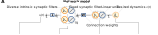
\includegraphics{media/chapters/04_temporal_tuning/feed_forward_dynamics.pdf}\\[-0.875em]
	\includegraphics{media/chapters/04_temporal_tuning/feed_forward_dynamics_plots.pdf}
	\caption[Solving for desired dynamics in a feed-forward linear network]{Solving for desired dynamics in a feed-forward linear network.
	\textbf{(A)} Overview of the network architecture. 
	A collection of $q$ synaptic filters diversifies the temporal response in a pre-population.
	%Due to linearity of the network, we can move the connection weight matrix $\mat B$ past the post-population.
	\textbf{(B, C, D, E)}~Example with $q = 4$ first-order low-pass filters (time-constants $\SI{10}{\milli\second}$, $\SI{22}{\milli\second}$, $\SI{46}{\milli\second}$, and $\SI{100}{\milli\second}$).
	The desired dynamics are a high-pass filter (eq.~\ref{eqn:high_pass}, $\tau_1 = \SI{20}{\milli\second}$, $\tau_2 = \SI{40}{\milli\second}$, $\alpha = 1$).
	\emph{Top:} System response to a band-limited white noise signal $u(t)$.
	\emph{Bottom:} Impulse response.
	Dotted line in \emph{(E)} is the desired response, solid line is the response when solving for $\mat{W}$ using least squares.
	}
	\label{fig:feed_forward_dynamics}
\end{figure}

Assume that a pre-population possesses diverse temporal tuning.
We can now use \cref{eqn:weight_optimise_currents_temporal} to solve for desired post-population dynamics in feed-forward networks.
This is possible because the diverse temporal tuning of the pre-neurons forms a \emph{temporal basis}---just like the time-invariant tuning of an NEF population forms a basis from which arbitrary functions $f$ can be decoded (cf.~\Cref{fig:nef_transformation}).

\Cref{fig:feed_forward_dynamics} provides an example of this concept.
Each pre-population neuron possesses a slightly different synaptic filter time-constant, and we solve for weights that result in high-pass filter tuning of the post-population.
This is the same idea as in the time-cell model by \citet{howard2014unified}, although we take the synaptic filter of the post-population into account as well.

\begin{figure}[p]
	\centering
	
\includegraphics{media/chapters/04_temporal_tuning/feed_forward_low_pass_network.pdf}
	\includegraphics{media/chapters/04_temporal_tuning/feed_forward_low_pass.pdf}
	\caption[Chaining populations with diverse temporal tuning]{Chaining populations with diverse temporal tuning. \textbf{(A)}~Overview of the network architecture. Each population possesses $q = 100$ synaptic filters with time-constants between \SIrange{10}{100}{\milli\second}.
	The desired temporal tuning $\mathfrak{e}_i$ of each neuron is a \SI{5}{\milli\second} first-order low-pass filter.
	\textbf{(B)}~Impulse responses at different points in the network.
	Dotted lines correspond to the desired $\mathfrak{e}_i$.
	Connection weights were computed with perfect knowledge of the actual dynamics.
	Although the \SI{5}{\milli\second} filter can be decoded from the first population, the decoding error $E$ (\NRMSE) increases in subsequent populations (\emph{top}) and, as is apparent from the depicted spectra (\emph{bottom}), becomes a stronger low-pass.
	\label{fig:feed_forward_low_pass}
	}
\end{figure}

\subsubsection{Limitations of feed-forward dynamics}
As we alluded to when discussing the \citet{howard2014unified} time-cell model, there are major limitations to approximating dynamics in feed-forward networks---at least if we model synapses as low-pass filters.
Specifically, network dynamics slow down as the network depth increases, the memory of a fixed-depth network is finite, and, generally speaking, the set of linear dynamics that can be realised is rather limited.

Phrasing the first limitation more precisely, maintaining uniform dynamics across a series of chained populations becomes more difficult as the length of the chain increases.
This is illustrated in in \Cref{fig:feed_forward_low_pass}.
To reduce approximation errors, the desired temporal tuning for later populations must possess longer time-constants.
This is despite it being, perhaps counter-intuitively, possible to exploit the diverse synaptic filters and temporal tuning to realise dynamics with \emph{faster} time-constants than the fastest synaptic filter in the post-population.

\begin{figure}[p]
	\centering
	\includegraphics{media/chapters/04_temporal_tuning/low_pass_svd.pdf}
	\caption[Principal component analysis of a set of low-pass filters]{Principal component analysis of a set of low-pass filters. \textbf{(A)} Impulse responses of $q = 20$ synaptic low-pass filters. \textbf{(B, C)} First-order low-pass filter principal components and the corresponding normalised singular values. Most of the information is contained within the first $100$ milliseconds and only the first two to four orthogonal basis functions can be decoded stably. Increasing $q$ or increasing the range of possible $\tau$ does not substantially improve these numbers.}
	\label{fig:low_pass_svd}
\end{figure}

Conversely, pertaining our second limitation, it is not possible to solve for dynamics with \emph{slower} time-constants than what is dictated by the longest chain of synaptic filters.
Correspondingly, feed-forward dynamics cannot realise infinite-impulse-response dynamics such as ideal integrators and oscillators, and they are not a good model of phenomena such as working memory that rely on sustained neural activity.%
\footnote{Indeed, as elaborated by \citet[Section~8.4.1]{eliasmith2003neural}, local recurrent (and \emph{not} feed-forward) connections are known to generate sustained activity in biology (e.g., in eye-position control in goldfish, cf.~\cite{aksay2001vivo}).
However, recent studies also suggest that momentary synaptic adaptation outweigh persistent activities as a primary mechanism supporting working memory \citep{lundqvist2018working}.}
This is what \citet[Chapter~1, p.~4]{churchland1992computational} refer to when they claim that \enquote{complex effects are the outcome of the dynamics of neural networks} (see quote on the title page of this chapter).

Regarding the third issue, the set of possible dynamics that can be realised in feed-forward networks is severely limited.
We can analyse this by performing a principal component analysis (PCA) of low-pass filter impulse responses.
This \enquote{uncovers} the set of orthogonal temporal basis functions implicitly spanned by the low-pass filters; the associated singular values determine the contribution of each orthogonal basis function.
In the case of low-pass filters, and as is depicted in \Cref{fig:low_pass_svd}, the number of orthogonal basis functions that  substantially contributes to spanning the space is limited to about four; and those basis functions are most diverse over the first hundred milliseconds, indicating that this is the region where the basis is most \enquote{expressive}.
We analyse temporal bases in more detail in the next section.

\subsubsection{Recurrent connections}

Recurrent dynamics do not possess any of these limitations.
Specifically, recurrences can diversify the temporal tuning, even if, as in the NEF dynamics principle, the only temporal resource in a network are homogeneous synaptic filters.
%---this is, in a sense, exactly how we usually use the NEF dynamics principle.
%However, in constrast to principle three (cf.~\Cref{sec:nef_dynamics}), and as we demonstrate below, we can now naturally solve for weights that take heterogenous synaptic weights and higher order filters into account---without explicitly having to provide differentials of the input signals, as the closed-form solutions proposed by \cite{voelker2018improving} require.
% TODO: Note this in Section 2.3.3

Surprisingly, we do not have to take special precautions when solving for recurrent connection weights using \cref{eqn:weight_optimise_currents_temporal}---we simply treat the recurrent population as its own pre-population.
Correspondingly, as with any other pre-population, we assume that the population possesses the temporal tuning defined by the tuning-curve constraint (eq.~\ref{eqn:temporal_tuning_curve}).
We thus foster a self-fulfilling prophecy: we solve for dynamics assuming that the dynamics are already realised.

%It is worth recalling that this is one of the fundamental assumptions of the NEF.
%As we discussed in \Cref{sec:nef}, we assume that the pre-population tuning has been realised with a small error.
%This drastically simplifies solving for synaptic weights---specifically in the context of recurrent connections.

\begin{figure}
	\centering
	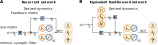
\includegraphics{media/chapters/04_temporal_tuning/recurrent_temporal_tuning.pdf}
	\caption[Solving for some desired temporal tuning in a recurrent neural network]{Solving for some desired temporal tuning in a recurrent neural network. \textbf{(A)} Overview of the recurrent neural network. We need to solve for an input matrix $\mat A$ and a feedback matrix $\mat B$ that realise the desired dynamics for the given intrinsic synaptic filter.
	\textbf{(B)} Assuming that the desired dynamics have already been realised, we obtain a feed-forward network.
	Solving for weight matrices is now a simple least-squares problem.
	Note that the placement of the weight matrices $\mat A$, $\mat B$ and the synaptic filters can be swapped because of linearity.
	}
	\label{fig:recurrent_temporal_tuning}
\end{figure}

Notably, this assumption effectively turns the system into a feed-forward network, greatly simplifying solving for recurrent weights (cf.~\Cref{fig:recurrent_temporal_tuning}).
In the special case of linear networks, solving for connection synaptic weights directly results in an input vector $\mat B'$ and a feedback matrix $\mat A'$.
If, as additional requirements, the synaptic filter is a first-order low-pass filter, and the system that is being realised is an LTI system, one can show that these matrices are equal to those returned by the NEF dynamics principle.
In other words, temporal tuning curves are a direct generalisation of the standard NEF methods.

\begin{restatable}{theorem}{thmTemporalLstsq}
	\label{thm:temporal_lstsq}
	Let $\mat A \in \mathbb{R}^{n \times n}$, $\mat B \in \mathbb{R}^n$ represent a stable LTI system, $\mathfrak{e}_i$ be the impulse response of its $i$th state dimension, and $h(t)$ is the impulse response of a first-order low-pass:
	\begin{align*}
		  \dot{\vec m}(t) &= \mat A \vec m(t) + \mat B \vec u(t)  \,, 
		& \mathfrak{e}_i(t) &= \big(\!\exp( \mat A t ) \mat B \big)_i \,,
		& h(t) &= \tau^{-1} e^{-t \tau^{-1}} \,.
	\end{align*}
	Let $\mathfrak{x}_k : \mathbb{R}^- \to \mathbb{R}$ be one of $N \geq n + 1$ arbitrary (with some mild constraints; see proof) input signals.
	If all $\mathfrak{e}_i$ and $\mathfrak{x}_k$ are pairwise linearly independent, $\mathfrak{e}_i$ the following least-squares loss has a unique minimum at $(b'_{i}, a'_{i, 1}, \ldots, a'_{in}) = ( \mat B', \mat A' )_i$ for all $i \in \{1, \ldots, n\}$, where $\mat A' = \tau \mat A + \mat I$, $\mat B' = \tau \mat B$:
	\begin{align*}
		E &=\sum_{k = 1}^{N} \left(
					\int_{0}^{\infty} \!\! \mathfrak{e}_i(\tau) \mathfrak{x}_k(-\tau)
		          - b'_{i} h(\tau) \mathfrak{x}_k(-\tau)
		          - \sum_{j=1}^n a'_{ij} h(\tau) \int_0^\infty \!\! \mathfrak{x}_k(-\tau - \tau') \mathfrak{e}_j(\tau') \, \mathrm{d}\tau' \mathrm{d}\tau \right)^2 \,.
	\end{align*}
\end{restatable}
\noindent This loss function is equal to \cref{eqn:weight_optimise_currents_temporal} in the case of a linear network with $n$ neurons that recurrently connect to themselves, and a \enquote{zeroth} pre-neuron with no temporal tuning providing input, i.e., $a_0(t) = \mathfrak{x}_k(t)$.
We provide a proof for this in \Cref{app:lstsq_nef_equivalence}.
%Note that the requirement for linearly independent samples is a mere technicality; different $\mathfrak{x}_k$ could in theory map onto the same sample points if the $\mathfrak{e}_i$ are periodic.

\begin{figure}[p]
	\centering
	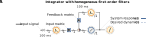
\includegraphics{media/chapters/04_temporal_tuning/recurrence_examples_a_diagram.pdf}\\[0.5em]
	\includegraphics{media/chapters/04_temporal_tuning/recurrence_examples_a.pdf}\\[1em]
	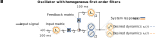
\includegraphics{media/chapters/04_temporal_tuning/recurrence_examples_b_diagram.pdf}\\[0.5em]
	\includegraphics{media/chapters/04_temporal_tuning/recurrence_examples_b.pdf}%
	{\phantomsubcaption\label{fig:recurrence_examples_1a}}%
	{\phantomsubcaption\label{fig:recurrence_examples_1b}}%
	\caption[Realising LTI systems using temporal tuning curves]{
		Realising LTI systems using temporal tuning curves.
		The depicted networks possess homogeneous first-order low-pass filters as synaptic filters.
		The computed matrices $\mat A$, $\mat B$ are equal to the matrices obtained using the NEF dynamics principle down to two decimal places.
		We use $N = 1000$ input signals $\mathfrak{x}_k$ of length $T = \SI{10}{\second}$ sampled at $\Delta t = \SI{1}{\milli\second}$ consisting of white noise filtered with a second-order low-pass filter (time constant $\vartheta = \SI{100}{\milli\second}$).
		Error values $E$ are the \NRMSE.
		\textbf{(A)} Realising an integrator (step impulse-response).
		Note that the system settles at a value slightly smaller than one for a unit pulse input (\emph{left}) due to the aforementioned imprecisions. For a white-noise input (\emph{right}) the result is effectively indistinguishable from the ground-truth solution.
		\textbf{(B)}~Realising a harmonic oscillator by solving for the impulse response of the two-state variables.
		Again, the solution is slightly imprecise causing a small frequency shift.
		In addition, in the case of the unit pulse input (\emph{left}), the system slowly diverges.
	}
	\label{fig:recurrence_examples_1}
\end{figure}

Examples of LTI systems realised by solving the least-squares loss are depicted in \Cref{fig:recurrence_examples_1}.
Note that there are some minor discrepancies between the numerical and the ideal solution (error is on the order of $10^{-3}$).
These errors are mostly due to time-discretisation at $\Delta t = \SI{1}{\milli\second}$, and would be less noticeable for exponentially decaying impulse responses $\mathfrak{e}_i$.

\subsection{Realising LTI Systems in Networks With More Complex Recurrences}
\label{sec:lti_complex_networks}

Admittedly, the results presented in the previous subsection are slightly underwhelming.
Solving for the dynamics numerically is computationally expensive,%
\footnote{On the order of one second per processor core, neuron and synaptic filter for $N = {1000}$, $T = \SI{1}{\second}$, $\Delta t = \SI{1}{\milli\second}$.}
and the resulting matrices $\mat A$, $\mat B$ are only precise to about two decimal places (i.e.,~an error of about $10^{-3}$).
%We could obtain better results by just using the closed-form solution.

Still, there are two reasons why our approach is useful.
First, the imprecisions are negligible compared to those resulting from implementing a linear transformation in a spiking neural network.%
\footnote{For $n \approx 100$ neurons, errors due to noise are on the order of $10^{-2}$, whereas errors due to static distortion are on the order of~$10^{-3}$ \citep[cf.][Section~2.2.2 and Figure~2.6, note the squared errors]{eliasmith2003neural}.}
Second, and most importantly, the strength of our approach lies in being agnostic to the network architecture; we can approximate connection weights for networks with higher-order and heterogeneous synaptic filters in the feedback and input paths.

\begin{figure}[p]
	\centering
	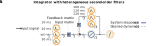
\includegraphics{media/chapters/04_temporal_tuning/recurrence_examples_c_diagram.pdf}\\[0.5em]
	\includegraphics{media/chapters/04_temporal_tuning/recurrence_examples_c.pdf}\\[1.45em]
	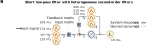
\includegraphics{media/chapters/04_temporal_tuning/recurrence_examples_d_diagram.pdf}\\[0.5em]
	\includegraphics{media/chapters/04_temporal_tuning/recurrence_examples_d.pdf}
	{\phantomsubcaption\label{fig:recurrence_examples_2a}}%
	{\phantomsubcaption\label{fig:recurrence_examples_2b}}%
	\caption[Realising LTI systems in networks with heterogeneous second-order filters]{Realising LTI systems in networks with heterogeneous second-order filters.
	The depicted networks possess a single linear neuron with multiple heterogeneous synaptic filters.
	The grey line corresponds to a reference solution obtained with a single second-order filter in each path.
	Same setup and legend as described in \Cref{fig:recurrence_examples_1}.
	\textbf{(A)} Implementing an integrator; the pre-synaptic time-constants are much shorter than the post-synaptic time-constants.
	Using \cref{eqn:weight_optimise_currents_temporal}, it is possible to solve for quite precise integrator dynamics.
	\textbf{(B)} Implementing a first-order low-pass with $\tau = \SI{10}{\milli\second}$ in a network with much longer synaptic filters.
	While the response to band-limited white noise (\emph{right}) is reasonably good, there are severe ringing artefacts at input transients, e.g., in the unit pulse (\emph{left}).
	}
	\label{fig:recurrence_examples_2}
\end{figure}

\begin{figure}
	\centering
	\includegraphics{media/chapters/04_temporal_tuning/heterogeneous_recurrence_exploration.pdf}
	\caption[Approximation errors in heterogeneous networks with second-order synaptic filters]{Approximation errors in heterogeneous networks with second-order synaptic filters.
	Errors are the median NRMSE between the actual and desired response for bandlimited white-noise input over $1000$ trials.
	Dotted orange lines correspond to feed-forward networks; blue lines to recurrent networks.
	See \Cref{fig:recurrence_examples_2} for the architecture and the minimum/maximum filter time constants in each path.
	Dashed line is a reference network with homogeneous first-order filters ($\tau = \SI{100}{\milli\second}$).
	Shaded areas are the $25$th and $75$percentiles.
	Same training procedure as in \Cref{fig:recurrence_examples_1}; training signals $\mathfrak{x}_k$ are white noise filtered with a second-order low-pass filter with time constant \SI{100}{\milli\second}.
	\textbf{(A)}~Implementing an integrator.
	Recurrence is required to implement the integrator.
	\textbf{(B)}~Emulating a $\SI{10}{\milli\second}$ first-order low-pass well requires recurrence and two or more filters per path.
	}
	\label{fig:heterogeneous_recurrence_exploration}
\end{figure}

\subsubsection{Realising integrators and low-pass filters in heterogeneous networks}
To demonstrate this, we next analyse networks with second-order synaptic filters (cf.~\cref{sec:synaptic_transmission}; \cref{eqn:low_pass_second_order}) and long, heterogeneous time-constants $\tau$.
Results are depicted in \Cref{fig:recurrence_examples_2,fig:heterogeneous_recurrence_exploration}.
%\begin{align}
%	h(t) &= \frac{t^n}{n! \tau^{n + 1}}  e^{-\frac{t}{\tau}} \,, & H(s) &= \frac{1}{(1 + \tau s)^{n + 1}} \,, & \text{where } n = 1 \text{ results in a second-order filter} \,.
%\end{align}
Our goal is to implement an integrator and a short first-order low-pass filter with $\tau = \SI{10}{\milli\second}$.
Importantly, being able to realise these systems implies that we can implement any LTI system.%
\footnote{This follows from the controllable canonical form \citep[cf.][Section~3.4.4]{verhaegen2007filtering}, which can be interpreted as chain of leaky integrators (i.e., low-pass filters).}

As is depicted in \Cref{fig:heterogeneous_recurrence_exploration}, the system performance critically depends on placing \emph{multiple} filters with different time-constants in the input and feedback path.%
\footnote{Multiple synaptic filters per connection are technically not compatible with the way our optimisation problem is phrased in \cref{eqn:weight_optimise_currents_temporal}.
However, we can assume that the different feed-forward filters correspond to diverse temporal tuning of different pre-population neurons, and the different recurrent filters could are obtained by simply splitting our single neuron into three with the same desired temporal tuning.}
Curiously, this is \emph{more} biologically plausible, since there typically is some variance in synaptic time-constants in biology \citep{jones2014neurotransmitter}.
For the integrator, increasing the number of filters reduces the error by up to two orders of magnitudes, well below what could be realised in a spiking neural network for input bandwidths up to \SI{100}{\hertz}.
The \enquote{short low-pass} system only performs well for input frequencies up to \SI{10}{\hertz}, but similarly requires at least two filters per path.

The necessity for multiple filters follows from \citet[Section~4.4, p.~591]{voelker2018improving}.
To realise a dynamical system with an $n$th order synaptic filter, we must generally provide the first $n - 1$ time-dervatives of the input to the network, i.e., $\mathrm{d} / \mathrm{d} t \, \mathfrak{x}$, $\ldots$, $\mathrm{d} / \mathrm{d} t^{n - 1} \, \mathfrak{x}$.
Accounting for heterogeneous filters similarly requires access to the derivative (cf.~\Cref{app:heterogenous_time_constants}).

The different filters in the feed-forward path can be thought of being linearly combined to \emph{approximate} these differentials, akin to the \enquote{dual-time-constant networks} explored by \citet{tripp2010population}.
Numerically solving the weight optimisation problem in \cref{eqn:weight_optimise_currents_temporal} automatically determines the weights that implicitly decode the differentials and that, at the same time, \emph{approximate} the desired dynamics.

\begin{figure}
	\centering
	\includegraphics{media/chapters/04_temporal_tuning/heterogeneous_recurrence_exploration_xs_flt.pdf}
	\caption[Effect of the input signal distribution the system error]{Effect of the input signal distribution the system error.
	Same setup and legend as in \Cref{fig:heterogeneous_recurrence_exploration}, but for a recurrent network with three filters and with input signals $\mathfrak{x}_k$ of varying bandwidth.
	Inputs are generated by low-pass filtering white noise with a second-order low-pass; the time-constant $\rho$ of that filter corresponds to the different line colours (dark blue corresponds high-bandwidth signals, orange to low-frequency signals).
	Data is the median over $1000$ trials, shaded areas are the $25$th and $75$th percentile.
	\textbf{(A)}~For the integrator, there is a trade-off between lower errors in a small frequency range, and larger, but consistent errors.
	\textbf{(B)}~The input distribution has a smaller effect on this network; the optimal solution is mostly independent of the input.
	}
	\label{fig:heterogeneous_recurrence_exploration_xs_flt}
\end{figure}

\subsubsection{Impact of the training samples $\mathfrak{x}_k$}
The emphasis on \enquote{approximate} is important here.
In contrast to the heterogeneous networks with first-order synaptic filter discussed in the context of \Cref{thm:temporal_lstsq}, there are no guarantees that the final network dynamics are \emph{exactly} the desired dynamics.
Moreover, the ability of the network to generalise depends on the input signals $\mathfrak{x}_k$ used for training.
While this is the norm in most machine learning scenarios, the network in \Cref{thm:temporal_lstsq} did not have this constraint (cf.~\Cref{app:temporal_tuning_proofs}).

We explore the effect of the training signals on the final network in \Cref{fig:heterogeneous_recurrence_exploration_xs_flt}.
Specifically, we generate $\mathfrak{x}_k$ with different frequency content by varying the time-constant $\rho$ of the second-order low-pass filter that is applied to the generated white noise.
Unsurprisingly, only supplying low-frequency inputs (i.e., using a large $\rho$) results in networks that achieve low errors for low-frequency inputs.
A more wide-band input (i.e., using a small $\rho$) results in a compromise-solution with smaller errors for wide-band inputs, but (at least in the case of the integrator) both slightly higher errors for low-frequency inputs.

\subsubsection{Relationship to system identification}
When solving for weights in a recurrent system using \cref{eqn:weight_optimise_currents_temporal}, we do not have any formal guarantee that the resulting system is stable---that is, unless the desired dynamics are stable and can be approximated \emph{precisely}.
While, judging from our experience, exponentially decaying temporal tuning curves $\mathfrak{e}_i(t)$ result in stable network, it would be good to be able to characterise this more thoroughly.

While we are still working on a more thorough analysis, we can at least draw some interesting parallels to the problem of least-squares system identification \citep[cf.][specifically Chapters~7-10]{verhaegen2007filtering}.
That is, we can treat the desired dynamics $\mathfrak{e}_i(t)$ as if they were the output of a black-box system in response to our input signals $\vec{\mathfrak{x}}_k(t)$.
Our goal is to find model parameters $w_{ij}$ that predict the observed output.%
\footnote{In our specific system identification problem is less complex than a general problem.
We directly measure the state, and we do not have instantaneous impulse responses.
Put differently, the output matrix $\mat C$ of our LTI system is the identity, and the feedthrough matrix $\mat D$ is zero.}

In fact, our optimisation problem in \cref{eqn:weight_optimise_currents_temporal} is a variant of the \enquote{integral-equation approach to system identification} presented by \citet{whitfield1987integralequation}, and, in less developed form, by \citet{squire1971simple}.
The primary difference to our approach is that our networks do not contain perfect integrators---correspondingly, we convolve the with the synaptic filter instead of integrating.
This is possible because the integral-equation approach is---at least if the system can be perfectly realised---invariant to convolution with a non-zero filter.

A central challenge of the integral-equation approach is robustness to noise in the measurements, which---even in the case of zero-mean white noise---causes asymptotic biases in the resulting system \citep{sagara1989recursive}.
That is, even as the number of samples $N$ goes to infinity, the estimated system parameters differ from the true system parameters.
Given that we mostly work with artificially generated data, the primary source of noise is time-discretisation.
It may be possible to incorporate more modern weight solving approaches with imposed stability guaranties, as is discussed in \citet{verhaegen2007filtering}.

\subsubsection{Realising dynamics in recurrences with intermediate populations}

\begin{figure}
	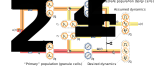
\includegraphics{media/chapters/04_temporal_tuning/recurrent_network_intermediate.pdf}
	\caption[Approximating dynamical systems across intermediate populations]{Approximating dynamical systems across intermediate populations. Both neuron populations receive input $u(t)$ through a set of synaptic filters with time-constants $\tau_1$, $\tau_2$; the upper, or \enquote{intermediate} population then projects onto the lower population, the lower population provides the output and projects onto the upper population. Each feedback path passes through another set of filters with time-constant $\tau_2$, $\tau_3$.
	As before, we can solve for connection weights $\mat A_1'$, $\mat A_2'$, $\mat B_1'$, $\mat B_2'$ by assuming that the desired dynamics have already been realised (scissor symbol and dotted lines).
	We must then account for all possible paths (coloured backgrounds) from the input $u(t)$ to the output $\vec m(t)$.
	}
	\label{fig:recurrent_network_intermediate}
\end{figure}

So far, we assumed that recurrent connections are tight loops that originate in a certain population and laterally target neurons in the same population.
This is not necessarily the case in biology.
As we mentioned in the context of Dale's principle in \Cref{sec:nef_limitations,sec:nef_nonneg}, inhibitory input passes through interneuron populations.
Fortunately, the interneurons typically do not dramatically affect the overall network dynamics \citep{parisien2008solving}.

There are, of course, exceptions to this.
As we discuss in more detail in \Cref{chp:cerebellum}, the Granule-Golgi microcircuit in the cerebellum possesses relatively slow synapses in the connection from the excitatory granule cells to the inhibitory Golgi cells.%
\footnote{As reported by \citet{dieudonne1998submillisecond}, the synaptic dynamics of the granule to Golgi projection can be modelled using second order filter dynamics and time constants of $\tau_1 \approx \SI{31}{\milli\second}$ and $\tau_2 \approx \SI{170}{\milli\second}$ (cf.~\cref{eqn:low_pass_second_order}); this corresponds to a first-order low-pass filter with a time constant of about \SIrange{60}{70}{\milli\second}.}
Additionally, the interneurons receive the same input $u(t)$ as the excitatory population \citep{dangelo2013cerebellar}, which does not fit our canonical picture of interneuron populations.

\Cref{fig:recurrent_network_intermediate} illustrates this \enquote{Granule-Golgi circuit} schematically.
To realise an LTI system $\mat A$, $\mat B$ in such a circuit, we must find weight matrices $\mat A_1'$, $\mat A_2'$, $\mat B_1'$, $\mat B_2'$ that compensate for the network dynamics.
We next discuss two ways to approach this problem.

\begin{figure}
	\includegraphics{media/chapters/04_temporal_tuning/recurrence_example_intermediate.pdf}
	\caption[Realising an integrator in a recurrent network with an intermediate population]{Realising an integrator in a recurrent network with an intermediate population and heterogeneous synaptic filters. Same experimental setup as in \Cref{fig:recurrence_examples_1}; errors $E$ are the \NRMSE.
	\textbf{(A)}~A single filter per path ($\tau_1 = \tau_4 = \SI{10}{\milli\second}$, $\tau_2 = \tau_3 = \SI{100}{\milli\second}$).
	Errors are relatively large, since we do not compensate for the second-order filter formed by the filter-chain.
	\textbf{(B)} Placing three filters in each path (for a total of $21$ weights) results in smaller errors (time-constants are between \SIrange{10}{30}{\milli\second} in the input path, and \SIrange{100}{120}{\milli\second} in the recurrent path).
	We sidestep splitting the computed weight matrices by simulating a partially collapsed network; this has no influence on the network function.
	}
	\label{fig:recurrence_example_intermediate}
\end{figure}

\paragraph{Subscribing temporal tuning to the interneuron population}
First, we could simply decide on some temporal tuning for the interneuron population and use \cref{eqn:weight_optimise_currents_temporal} to solve for connection weights.
If both neuron populations possess the same temporal tuning, then the interneurons appear as a pass-through to the primary population.
Assuming homogeneous first-order synaptic filters with time-constant $\tau$, the closed-form solution is
\begin{align}
	\mat A_1' &= \mat A_2' = \tau \mat A + \mat I \,, & \mat B_1' &= \mat B_2' = \tau \mat B \,.
\end{align}
Put differently, we use the closed-form solution from the \NEF dynamics principle in both paths.
This makes intuitive sense due to symmetry, but see \Cref{app:granule_golgi_dynamics} for a detailed derivation.

\paragraph{Unrolling the network}
An alternative approach is to solve for all weights simultaneously.
Assuming that we have already realised the desired tuning at the output of the network, and because all our neurons and filters are linear (cf.~the beginning of \Cref{sec:temporal_tuning_lti}), we can \enquote{unroll} the network into several feed-forward paths (coloured in \Cref{fig:recurrent_network_intermediate}).

Let $h_1$, $\ldots$, $h_4$ denote the individual synaptic filters.
Furthermore, to simplify our notation, let $\mathfrak{e}$ be a vectorial function $\mathfrak{e} : \mathbb{R}^+ \longrightarrow \mathbb{R}^q$, and let \enquote{$\ast$} denote elementwise convolution.
We obtain the following loss function:
{%
%\newcommand{\pathOne}[1]{\mbox{\colorbox{IndianRed}{$\displaystyle {#1}$}}}%
%\newcommand{\pathTwo}[1]{\mbox{\colorbox{Gold}{$\displaystyle {#1}$}}}%
%\newcommand{\pathThree}[1]{\mbox{\colorbox{YellowGreen}{$\displaystyle {#1}$}}}%
\newcommand{\pathOne}[1]{#1}%
\newcommand{\pathTwo}[1]{#1}%
\newcommand{\pathThree}[1]{#1}%
\begin{align}
	E = \sum_{k = 1}^N \, \bigl\| \, (\mathfrak{x}_k \ast \mathfrak{e})(0)
		- \pathOne{\mat{B}_2' (h_4 \ast u)(0)}
		- \pathTwo{\mat{A}_1' \mat{B}_1' \bigl(h_3 \ast (h_1 \ast u)\bigr)(0)}
		- \pathThree{\mat{A}_1' \mat{A}_2' \bigl(h_3 \ast (h_2 \ast \mathfrak{e})\bigr)(0)}
	\, \bigr\|_2^2 \,.
\end{align}}%
Minimising this loss function results in the matrix products $\mat{A}_1' \mat{A_2}'$ and $\mat{A}_1' \mat{B}_1'$ instead of the individual matrices; however, the weights can be split arbitrarily in a post-processing step.
\Cref{fig:recurrence_example_intermediate} depicts the results of realising an integrator using this method.


\clearpage
\setcounter{section}{1}
% !TeX spellcheck = en_GB

\section{Realising Temporal Bases}
\label{sec:temporal_bases}

\newcommand{\cPos}[1]{\textbf{\textcolor{DarkBlue}{#1}}}
\newcommand{\cNeg}[1]{\textbf{\textcolor{DarkRed}{#1}}}

In the previous section, we demonstrated that feed-forward networks alone are insufficient to explain the complex dynamics observed in biological systems.
However, we also demonstrated that we can realise arbitrary LTI systems of the form $\dot{\vec m}(t) = \mat A \vec m(t) + \mat B u(t)$ in recurrent \emph{linear} networks.
While we show in the next section that we can successfully solve for dynamics in networks with nonlinear neurons, our goal for now is to consider what specific temporal tuning we should \emph{optimally} realise, and how to translate this tuning into an LTI system.

As we already mentioned above, implementing an LTI system in a recurrent connection can diversify the available temporal tuning.
This in turn allows us to decode a wider range of dynamics in ensuing feed-forward sections of the network.
To maximise the set of dynamics that can be decoded, and without further knowledge about the input signals, we should optimally realise $q$ orthonormal temporal encoders $\mathfrak{e}_1(t)$, $\ldots$, $\mathfrak{b}_q(t)$ over an interval $t \in [0, \theta]$.
Orthonormality ensures that the $\mathfrak{e}_i$ are not redundant.

We first describe our overall goal more precisely, namely constructing LTI systems that approximate sliding-window spectra.
We then review common continuous and discrete bases, and discuss two methods for constructing LTI systems that generate these bases: numerically optimising an autoregressive model, and analytically solving for LTI systems generating the Legendre basis.
This latter approach yields a novel derivation of the Legendre Delay Network (LDN; \cite{voelker2018improving}) and is conceptually similar to work by \citet{gu2020hippo}.
Finally, we compare the bases generated by these systems in terms of their expressiveness.

\subsection{Computing Sliding-Window Spectra using Linear Time-Invariant Systems}
\label{sec:sliding_window_lti}

Given a function basis spanning a space such as $L^2(0, \theta)$ (cf.~\Cref{app:functional_analysis}), any function $\mathfrak{f} \in L^2(0, \theta)$ can be represented as an infinite weighted sum of basis functions $\mathfrak{b}_n$.
In the case of an orthonormal function basis (i.e., $\langle \mathfrak{b}_i, \mathfrak{b}_j \rangle = \delta_{ij}$), the corresponding weights $\chi_i$ \emph{uniquely} define each $\mathfrak{f}$ and are referred to as \emph{generalised Fourier coefficients} or the \emph{spectrum} of $\mathfrak{f}$:

\begin{definition}[{Generalised Fourier series and coefficients; cf.~\cite{young1988introduction}, Definition 4.3}]
Consider an orthonormal function basis $(\mathfrak{b}_n)_{n \in \mathbb{N}}$, where each $\mathfrak{b}_n \in L^2(0, \theta)$, as well as a function $\mathfrak{f} \in L^2(0, \theta)$. 
Then the series
\begin{align}
	\mathfrak{f} &= \sum\nolimits_{i = 0}^\infty \langle \mathfrak{f}, \mathfrak{b}_i \rangle \mathfrak{b}_i = \sum\nolimits_{i = 0}^\infty \chi_i \mathfrak{b}_i
	\label{eqn:generalised_fourier_coefficients}
\end{align}
is the generalised Fourier series of the given $\mathfrak{f}$ and $\chi_i$ are the generalised Fourier coefficients.
\end{definition}

\subsubsection{Note on using a finite number of basis functions}
In practice, it is often infeasible to realise an infinite number of basis functions.
While the $\mathfrak{b}_n$ are not necessarily ordered---any permutation $(\mathfrak{b}_{\pi(n)})_{n \in \mathbb{N}}$ still forms a valid basis---the basis functions we discuss in this section are arranged such that larger $n$ correspond to higher frequency content.
Correspondingly, only using the first $q$ basis functions results in a negligible reconstruction error if our signals are bandlimited, or, equivalently, our signals and bases are discretised appropriately (see below).

\subsubsection{Sliding-window spectrum}
Coming back to the generalised Fourier coefficients $\chi_i$, note that the inner product $\langle \mathfrak{f}, \mathfrak{b}_i \rangle$ is---time-reversal aside---merely a convolution between $\mathfrak{f}$ and $\mathfrak{b}_i$:
\begin{align*}
	\chi_i = \langle \mathfrak{f}, \mathfrak{b}_i \rangle = \int_0^\theta \!\! \mathfrak{f}(\tau) \mathfrak{b}_i(\tau) \, \mathrm{d}\tau = (\bar{\mathfrak{f}} \ast \mathfrak{b}_i)(0) \quad \quad \text{where } \bar{\mathfrak{f}}(t) \mapsto \mathfrak{f}(-t) \,.
\end{align*}
Correspondingly, if we were able to realise an LTI system that has $q$ orthonormal basis functions $\mathfrak{b}_i$ as an impulse response over a window $[0, \theta]$, then the state $\vec m(t)$ of that system would correspond to the generalised Fourier coefficients $\chi_i$ representing the past $\theta$ seconds of $u(t)$, which we denote as $u_{[t - \theta, t]} : [-\theta, 0] \longrightarrow \mathbb{R}$ with $u_{[t - \theta, t]}(\tau) \mapsto u(t + \tau)$:
\begin{align*}
	m_i(t) &= \int_0^\theta \!\! u(t - \tau) \mathfrak{b}_i(\tau) \, \mathrm{d}\tau
	        = \int_0^\theta \!\! u_{[t - \theta, t]}(-\tau) \mathfrak{b}_i(\tau) \, \mathrm{d}\tau
	        = \langle \bar u_{[t - \theta, t]}, \mathfrak{b}_i \rangle  \,.
\end{align*}
This is sometimes referred to as a \emph{sliding-window spectrum} \citep{bastiaans1985slidingwindow,denbrinler1996generalized}.%
\footnote{The cited publications use this term in the context of discrete signals, but the concept is the same.}
We illustrate this concept in \Cref{fig:lti_basis_trafo_a,fig:lti_basis_trafo_b,fig:lti_basis_trafo_c}.

\begin{figure}
	\centering
	\includegraphics{media/chapters/04_temporal_tuning/lti_basis_trafo.pdf}%
	{\phantomsubcaption\label{fig:lti_basis_trafo_a}}%
	{\phantomsubcaption\label{fig:lti_basis_trafo_b}}%
	{\phantomsubcaption\label{fig:lti_basis_trafo_c}}%
	{\phantomsubcaption\label{fig:lti_basis_trafo_d}}%
	\kern-158mm\includegraphics{media/chapters/04_temporal_tuning/lti_basis_trafo_plots.pdf}\\[0.3cm]
	\caption[Using an LTI system to compute a sliding basis transformation]{Using an LTI system $\dot{\vec m}(t) = \mat A \vec m(t) + \mat B u(t)$ to compute a sliding-window spectrum.
	\textbf{(A)} Any LTI system can either be implemented as using an integrator with feedback, or, as is depicted in \textbf{(B)}, by convolving $u(t)$ with the impulse response $\mathfrak{b}_i$ of each state dimension.
	\textbf{(C)} Assume that $\mathfrak{b}_i$ was a basis function over a window $[0, \theta]$.
	Then, each state dimension $m_i(t)$ is the convolution between $\mathfrak{b}_i$ and a slice of the input signal $u_{[t - \theta, t]}$.
	Correspondingly, $m_i(t)$ is the generalised Fourier coefficient $\chi_i$ describing $u_{[t - \theta, t]}$ in terms of the function basis \emph{at each point in time}.
	In other words, $\vec m(t)$ contains a compressed representation of $u_{[t - \theta, t]}$.
	\textbf{(D)} By linearly combining $\vec m(t)$ using a \enquote{decoding} matrix $\mat C$, we can approximate another LTI system, for example a delay $y(t) \approx u(t - \theta / 2)$.
	}
	\label{fig:lti_basis_trafo}
\end{figure}

\subsubsection{Transforming the sliding-window spectrum}
Another way to interpret $\vec m(t)$ is as a compressed representation of $u_{[t - \theta, t]}$.
That is, realising $q$ temporal basis functions as an LTI system continuously compresses $u_{[t - \theta, t]}$ into a $q$-dimensional vector $\vec m(t)$.
Specifically, for $q \to \infty$, and as is suggested by \cref{eqn:generalised_fourier_coefficients}, we can perfectly reconstruct $u_{[t - \theta, t]}$ from $\vec m$:
\begin{align*}
	u_{[t - \theta, t]}(-\tau) &= \sum_{i = 0}^\infty m_i \mathfrak{b}_i(\tau) = \sum_{i = 0}^\infty \langle \bar u_{[t - \theta, t]}, \mathfrak{b}_i \rangle \mathfrak{b}_i(\tau) \quad\quad \text{where } 0 \leq \tau \leq \theta \,.
\end{align*}
Similarly, we can compute $u(t)$ convolved with an arbitrary function $\mathfrak{c} : [0, \theta] \longrightarrow \mathbb{R}$ by linearly combining the entries of $\vec m(t)$.
Let $\vec{c} = (c_0, c_1, \ldots) = \langle \mathfrak{c}, \mathfrak{b}_i \rangle$ be the generalised Fourier coefficients of $\mathfrak{c}$.
Then, $\langle \vec m(t), \vec{c} \rangle = (u \ast \mathfrak{c})(t)$:
\begin{align*}
	\langle \vec m(t), \vec{c} \rangle
		&= \sum_{i = 0}^\infty m_i(t) c_i
		 = \sum_{i = 0}^\infty \langle \bar u_{[t - \theta, t]}, \mathfrak{b}_i \rangle \langle \mathfrak{c}, \mathfrak{b}_i \rangle 
		 = \sum_{i = 0}^\infty \int_0^\theta \!\! \int_0^\theta \!\!
		 	\bigl( \bar u_{[t - \theta, t]}(\tau) \mathfrak{b}_i(\tau) \bigr)
		 	\bigl( \mathfrak{c}(\tau') \mathfrak{b}_i(\tau') \bigr) \,\mathrm{d}\tau \mathrm{d}\tau' \\
		&= \int_0^\theta \!\!
			\left(\sum\nolimits_{i = 0}^\infty m_i(t) \mathfrak{b}_i(\tau) \right)
			\left(\sum\nolimits_{i = 0}^\infty c_i \mathfrak{b}_i(\tau) \right) \,\mathrm{d}{\tau}
		 = \int_0^\theta \!\! u(t - \tau) \mathfrak{c}(\tau) \,\mathrm{d}{\tau}
		 = (u \ast \mathfrak{c})(t) \,.
\end{align*}
Where the step from the first to the second line follows from $\langle \mathfrak{b}_i, \mathfrak{b}_j \rangle = \delta_{ij}$.

An example of this is illustrated in \Cref{fig:lti_basis_trafo_d}, where we decode a delay $\mathfrak{c}(t) = \delta(t - \nicefrac{\theta}2)$ by linearly combining the three state dimensions $m_i(t)$.
Since $q = 3$ is finite, we cannot use $\vec c$ as defined above, but must instead solve the least-squares problem discussed in the context of approximating dynamics in feed-forward networks (i.e., eq.~\ref{eqn:weight_optimise_currents_temporal}).

For $q \to \infty$, $\vec m(t)$ represents all information in the windowed input signal $u_{[t - \theta, t]}$.
Correspondingly, we can compute any nonlinear function over $u_{[t - \theta, t]}$ by transforming $\vec m(t)$ nonlinearly.
We could, for example, represent $\vec m$ in a neuron population and decode a function $f(\vec m)$; if we learn this decoder online, we have an \emph{adaptive filter} (cf.~\Cref{sec:adaptive_filter}).

\subsection{Continuous and Discrete Orthonormal Function Bases}
\label{sec:function_bases}

\begin{figure}
	\includegraphics{media/chapters/04_temporal_tuning/continuous_bases.pdf}%
	{\phantomsubcaption\label{fig:fourier_series}}%
	{\phantomsubcaption\label{fig:cosine_series}}%
	{\phantomsubcaption\label{fig:legendre_series}}%
	\caption[Orthonormal basis functions]{
	Orthonormal basis functions. All plots are to scale, the dotted line is zero, ticks are $0$, $\theta$.}
\end{figure}

We next review three orthonormal bases spanning $L_2(0, 1)$: the Fourier and cosine series, as well as the shifted orthonormal Legendre polynomials.

\subsubsection{Fourier and cosine series}
The most prominent function basis for temporal representations is the Fourier series. This basis is closely related to the Fourier transformation.%
\footnote{While related, the Fourier series and Fourier transformation are different concepts.
The Fourier series spans a function space over $[0, 1]$, whereas the Fourier transformation maps functions $f : \mathbb{R} \longrightarrow \mathbb{C}$ onto functions $\mathcal{F}(f) : \mathbb{C} \longrightarrow \mathbb{C}$.
Still, the generalised Fourier coefficients $\chi_i$ of a function $f$ with respect to the Fourier series can be interpreted as the real and imaginary coefficients of the Fourier transformation for specific frequencies.}

\begin{definition}[Fourier series]

The Fourier series $(f_n)_{n \in \mathbb{N}}$ over $[0, 1]$ is given as
\begin{align}
		f_0(x) &= 1 \,,&
		f_{2n + 1}(x) &= \sqrt{2}\sin\bigl(2 \pi nx\bigr) \,, &
		f_{2n} &= \sqrt{2}\cos\bigl(2 \pi nx\bigr) \,.
		\label{eqn:fourier_series}
	\end{align}
\end{definition}

\noindent The first $f_i$ are depicted in \Cref{fig:fourier_series}.
Note the sine and cosine pairs, and that each function in the Fourier series is periodic over $[0, 1]$, that is $f_n(0) = f_n(1)$.
Correspondingly, if we truncate the Fourier series to $q$ terms, we can only represent periodic functions.

An arguably simpler alternative to the Fourier series is the cosine series.
This series skips the \enquote{sine} terms of the Fourier series and increments the frequency in steps of $\pi$ instead of $2\pi$.

\begin{definition}[Cosine series]
	The cosine series $(c_n)_{n \in \mathbb{N}}$ over $[0, 1]$ is given as
	\begin{align}
	 	c_0(x) &= 1 \,, &
	 	c_n(x) &= \sqrt{2}\cos(\pi n x) \,.
	 	\label{eqn:cosine_basis}
	\end{align}
\end{definition}

\noindent Again, the first $c_i$ are depicted in \Cref{fig:cosine_series}.
Since the cosine basis is aperiodic ($f_i(0) \neq f(1)$ for odd $i$), it is better suited to representing aperiodic functions if we only have a truncated basis with $q$ terms.
Natural signals are typically aperiodic with respect to a fixed sliding window.

\subsubsection{Polynomial bases}

An alternative to trigonometric bases are polynomial bases.
%\footnote{Confusingly, the Fourier and related series are sometimes referred to as \enquote{trigonometric polynomials}.}
Examples include the Legendre, Chebyshev, Laguerre, Hermite, and Jacobi polynomials (e.g., \cite{press2007numerical}, Section~4.6.1; \cite{arfken2005mathematical}, Chapter~12).
For our purposes, the Legendre basis is most interesting.
It is aperiodic, and in contrast to the other listed polynomial bases, orthogonal with respect to a constant weighting $W(x) = 1$.

\begin{definition}[Legendre polynomials]
\label{def:legendre_polynomial}
Legendre polynomials are uniquely defined as a sequence of functions $(p_n)_{n \in \mathbb{N}}$ over $[-1, 1]$ with the following properties: \emph{(1)} $p_n$ is a polynomial of order $n$, \emph{(2)} the $p_n$ are orthogonal ($\langle p_i, p_j \rangle = 0$ exactly if $i \neq j$), and \emph{(3)} $p_n(1) = 1\,$.
\end{definition}

\subsubsection{Recurrence relation}
Starting with the base cases $p_0(x) = 1$ and $p_1(x) = x$, the Legendre polynomials $p_n(x)$ are typically defined as a recurrence relation \citep[Section~4.6.1]{press2007numerical}:
\begin{align}
	(n + 1) p_{n + 1}(x) &= (2n + 1) x p_n(x) - n p_{n - 1}(x) \,.
	\label{eqn:leg_rec}
\end{align}
%Rewriting this in terms of the polynomial coefficients $\alpha_{n, i}$ (see above) we get
%\begin{align*}
% 	(n + 1) \alpha_{n + 1, i} &= \begin{cases}
% 		\hspace{6.6em} - \, n \alpha_{n - 1, i} & \text{if } i = 0 \,, \\
% 		(2n + 1) \alpha_{n, i - 1} - n \alpha_{n - 1, i} & \text{if } i > 0 \,.
% 	\end{cases}
%\end{align*}

\subsubsection{Closed form equation}
Alternatively, the \emph{orthonormal} shifted Legendre polynomial $\tilde p_n$ over $[0, 1]$ are given in closed form as
\begin{align}
   \tilde p_n(x) &= \sqrt{2n + 1} \, (-1)^n \sum_{i = 0}^n (-1)^i \binom{n}{i} \binom{n + i}{i} x^i \,.
   	\label{eqn:legendre_basis}
\end{align}
This basis is depicted in \Cref{fig:legendre_series}. It spans $L^2(0, 1)$, just like the Fourier and cosine basis.

\subsubsection{Discrete Orthonormal Function Bases}
Continuous basis functions are useful for mathematical analysis.
However, in practice, we often divide the interval $[0, 1]$ into $N$ individual samples.
Specifically, we use such discrete bases in our numerical method for deriving $\mat A$, $\mat B$, and at the end of this chapter in \Cref{sec:applications_to_ml}, when we discuss applications to machine learning.

Of course, from a mathematical perspective, the notion of \enquote{discrete function bases} is at most moderately exciting---once we discretise functions over an interval, we end up with finite-dimensional vector spaces over $\mathbb{R}^N$.
Still, there is some room for defining the concept of \enquote{discrete function bases} in relation to their continuous counterparts more rigorously.
Although our definitions are non-canonical, our notation roughly follows \citet{neuman1974discrete}.

\begin{definition}[Discrete Function Basis]
	\label{def:discrete_function_basis}
 	A \emph{discrete function basis} with an associated continuous function basis $(\mathfrak{b}_n)_{n \in \mathbb{N}}$ over $[0, 1]$ is a finite sequence of discrete basis functions $(E_n(k; N))_{n < N}$.
 	$n \in \{0, \ldots, N - 1\}$ is the basis function index, $k \in \{0, \ldots, N - 1\}$ is the sample index, and $N \geq 2$ is the number of samples.
 	The codomain of $E_n(k; N)$ is $\mathbb{R}$.
 	It must hold
 	\begin{align}
 		\lim_{N \to \infty} E_n \left( k; N \right) &= \frac{1}{\sqrt{N}} \mathfrak{b}_n\left(\frac{k}{N - 1}\right) \,, &
 		\text{and }
 		\sum_{k = 0}^{N - 1} E_i(k; N) E_j(k; N) &= \delta_{ij} \text{ if } E \text{ is orthonormal}\,.
 		\label{eqn:discrete_basis}
 	\end{align}
 	We call a matrix $\mat E \in \mathbb{R}^{q \times N}$ with $(\mat E)_{ij} = E_i(j; N)$ a \emph{basis transformation matrix}.
	In contrast to normal terminology we refer to $\mat E$ as \emph{orthonormal} if $\mat E^T \mat E = \mat I$, even if $\mat E$ is not square ($q < N$).
\end{definition}

Note that for $q = N$ an orthonormal basis transformation matrix $\mat E$ is an orthonormal basis of $\mathbb{R}^N$.
For $q < N$, the operation $\mat E \vec x$ lossily compresses $\vec x \in \mathbb{R}^N$ into a $q$-dimensional space.

\begin{figure}[t]
	\centering
	\includegraphics{media/chapters/04_temporal_tuning/discrete_basis_visualisation.pdf}%
	{\phantomsubcaption\label{fig:discrete_fourier}}%
	{\phantomsubcaption\label{fig:discrete_cosine}}%
	{\phantomsubcaption\label{fig:discrete_dlop}}%
	\caption[Visualisation of the discrete Fourier, cosine, and Legendre basis]{Visualisation of the discrete Fourier, cosine, and DLOP (Legendre) basis for $q = N = 40$.
	Each pixel is a separate sample. Red corresponds to negative values, blue to positive, grey to zero.}
\end{figure}

\subsubsection{Discrete Fourier and cosine basis}
Choosing the sample points carefully, we obtain the discrete Fourier $F_n$ and cosine bases $C_n$ used in the discrete Fourier and cosine transforms (DFT and DCT-II) and visualised in \Cref{fig:discrete_fourier,fig:discrete_cosine}:%
\footnote{
For even $N$, $F_{N - 1}$ must be rescaled to maintain orthonormality; we ignore this in our definition for terseness.
}
\begin{align}
  	F_0(k; N) &= \frac{1}{\sqrt{N}} \,, &
  	F_{2n + 1}(k; N) &= \frac{\sqrt{2}}{\sqrt{N}} \sin\left(
  		2 \pi n \frac{k + \frac{1}2}{N}\right) \,, &
  	F_{2n}(k; N) &= \frac{\sqrt{2}}{\sqrt{N}} \cos\left(
  		2 \pi n \frac{k + \frac{1}2}{N}\right) \,, \notag\\
  	C_0(k; N) &= \frac{1}{\sqrt{N}} \,, &
  	C_n(k; N) &= \frac{\sqrt{2}}{\sqrt{N}} \cos\left(\pi n \frac{k + \frac{1}2}{N}\right) \,.
  	\label{eqn:dft_dct}
\end{align}
In both cases, fast algorithms exist for computing $\mat F \vec x$ and $\mat C \vec x$ in $\mathcal{O}(N\log{N})$ instead of $\mathcal{O}(N^2)$, namely the FFT and FCT \citep[Chapter~12]{cooley1965algorithm,makhoul1980fast,press2007numerical}.

\subsubsection{Discrete Legendre Orthogonal Polynomials (DLOPs)}
A discrete version of the Legendre polynomials can be generated using the following recurrence relation (depicted in \Cref{fig:discrete_dlop}):
\begin{align*}
  	P_{0}(k; N) &= \frac{1}{\sqrt{N}} \,, \quad\quad
  	P_{1}(k; N)  = \frac{(2 k - N + 1)}{N - 1} \sqrt{\frac{3 (N - 1)}{N (N + 1)}} \,, \\
  	P_{n}(k; N) &= P_{n - 1}(k; N) \frac{(2n - 1) (N - 2k - 1)}{n (N - n)} \sqrt{\frac{\alpha_{n}(N)}{\alpha_{n - 1}(N)}}
                   - P_{n - 2}(k; N) \frac{(n - 1) (N + n - 1)}{n (N - n)} \sqrt{\frac{\alpha_{n}(N)}{\alpha_{n - 2}(N)}} \,.
\end{align*}
Where the normalisation factor $\alpha_n(N)$ is given as
\begin{align*}
 	\alpha_n(N) &= \frac{(2n + 1) (N - 1)^{(n)}}{(N + n)^{(n + 1)}} & \text{where } k^{(i)} &= \prod_{j = 0}^{i - 1} (k - j) = \frac{k!}{(k - i)!} \text{ is the $i$th fading factorial of $k$.}
\end{align*}
These \enquote{Discrete Legendre Orthogonal Polynomials} (DLOPs) have first been proposed by \citet{neuman1974discrete}.
Our modified recurrence relation above is numerically stable and directly produces an orthonormal basis. We provide a more detailed discussion in \citet{stockel2021discrete}.

\subsection{Numerically Solving for Linear Time Invariant Systems}
\label{sec:lti_autoregression}

Our next goal is to construct LTI systems $\dot{\vec m}(t) = \mat A \vec m(t) + \mat B u(t)$ that generate the above bases using only $q$ state dimensions.
To this end, we first describe a numerical method, and then, in the next subsection, analytically solve for $\mat A$, $\mat B$ in the specific case of the Legendre basis.

\subsubsection{Auto-regressive system identification}
Consider an orthonormal basis transformation matrix $\mat M \in \mathbb{R}^{q \times N}$. The $i$th column (with $i \in \{1, \ldots, N\}$) of $\mat M$, here denoted as $\vec m_i$, is a $q$-dimensional vector describing the impulse response of the desired system at $t = \Delta t i$, where $\Delta t = \theta / N$.
If this state evolution is indeed the result of a time-invariant linear process, then we have
\begin{align*}
	\vec m_0 &= \mat{\tilde B} \,, &
	\vec m_{i + 1} &= \vec m_{i} + \Delta t \mat{\tilde A} \vec m_i
	\quad \Leftrightarrow \quad
	\mat{\tilde A} \vec m_{i} = \frac{\vec m_{i + 1} - \vec m_i}{\Delta t} \quad \text{for all} \quad 1 \leq i < N \,,
\end{align*}
where $\mat{\tilde B}$ describes the influence of the initial impulse on the state, and $\mat{\tilde A}$ is the state-transition matrix.
Finding a $\mat{\tilde A}$ with this property can be written as a linear least-squares problem:
\begin{align}
	\mat{\tilde A} = \arg\min_{\mat{\tilde A}} \sum_{i = 1}^{N - 1} \left\| \mat{\tilde A} \vec m_i - \frac{\vec m_{i + 1} - \vec m_i}{\Delta t} \right\|_\mathrm{F}^2 \,.
	\label{eqn:construct_lti_lstsq}
\end{align}
This is a standard auto-regressive linear model \citep[cf.][Chapter~8]{verhaegen2007filtering}; of course, we could use the derivative of a continuous basis instead of the difference quotient.
Assuming that $\mat{\tilde A}$ and $\mat{\tilde B}$ are the result of discretising the LTI system with a zero-order hold assumption \citep[e.g.,][Section~9.8]{brogan1991modern}, we obtain a continuous system $\mat A$, $\mat B$ as follows:
\begin{align}
 	\mat A &= \frac{1}{\Delta t} \log\bigl(\mat I  + \Delta t \mat{\tilde A}\bigr) \,, &
 	\mat B &= \sqrt{N} \mat{\tilde B} \,,
 	\label{eqn:lti_inverse_discretisation}
\end{align}
where \enquote{$\log$} is the matrix logarithm, the inverse operation of taking the matrix exponential.
%Scaling $\mat{\tilde B}$ by $\sqrt{N}$ is necessary to obtain orthonormal basis functions.

\begin{figure}
	\centering
	\includegraphics{media/chapters/04_temporal_tuning/construct_lti.pdf}
	\caption[LTI systems generating the Fourier, cosine and Legendre basis]{LTI systems generating the Fourier, cosine and Legendre basis.
	Constructed using \cref{eqn:construct_lti_lstsq,eqn:lti_inverse_discretisation} and $N = 1000$ samples.
	\emph{Top:} NRMSE $E$ over $[0, \theta]$ between the LTI impulse response and the reference basis functions (excluding the constant $\mathfrak{b}_0$). Black cross is the mean, error bars the minimum and maximum error over $q - 1$ basis functions.
	\emph{Bottom:} First six dimensions of the reconstructed LTI system impulse response for $q = 11$ basis functions (cf.~above arrow); dotted line is the reference.
	\textbf{(A)} The Fourier basis can be constructed well by an LTI system for odd $q$ (mean $E < 10^{-2}$).
	\textbf{(B)} The cosine basis can only be realised as an LTI system with relatively large errors (mean $E > 10^{-1}$). Adding more basis functions reduces the error for earlier basis functions.
	\textbf{(C)} The Legendre basis can be realised well with small errors for all $q$ (mean $E < 2^{-2}$).
	}
	\label{fig:construct_lti}
\end{figure}

\Cref{fig:construct_lti} depicts the impulse responses of LTI systems constructed in this manner.
The method works well for the Fourier and the Legendre basis, but results in relatively large errors in the case of the cosine basis; particularly for later basis functions.
Since the Fourier system consists of $(q - 1) / 2$ harmonic oscillators requiring two state-dimensions each, $q$ must be odd.

Rather unsurprisingly, the impulse response of the generated LTI systems continues past the time-window $\theta$.
In the case of the Fourier and cosine basis, the oscillation just continues, whereas the Legendre system diverges.
To prevent this, we need to modify the system to rapidly decay to zero, preferably \emph{exactly} at time $\theta$.

\begin{figure}
	\centering
	\includegraphics{media/chapters/04_temporal_tuning/construct_lti_window.pdf}
	\caption[Windowed LTI systems generating the Fourier, cosine and Legendre basis]{
	Windowed LTI systems generating the Fourier, cosine and Legendre basis.
	Same experiment as in \Cref{fig:construct_lti_window}, but the target functions are multiplied with a linear window over $[0, \theta]$
	}
	\label{fig:construct_lti_window}
\end{figure}

\subsubsection{Window functions}
One possible solution is to multiply the desired basis with a window function $w(t) \in [0, 1]$, that is, $\mathfrak{b}'_i(t) = w(t) \mathfrak{b}_i(t)$ for $t \in [0, \theta]$.
Unfortunately, the resulting basis is no longer orthnormal, and decoding information in regions with small $w(t)$ is more difficult.

\Cref{fig:construct_lti_window} depicts results for a one-sided Bartlett window $w(t) = 1 - x \theta^{-1}$ \citep[cf.][Section~7.5]{oppenheim2009discretetime}.
Again, we are able to realise the desired dynamics well for the Fourier and Legendre basis, albeit with a large increase in error due to having to decode the window dynamics.
Furthermore, this method does not work particularly well for the cosine basis.
Although the final system is stable, we can still observe substantial oscillations for $t > \theta$.

\subsubsection{Establishing a rectangle window through \enquote{information erasure}}
Optimally, we would like to realise a rectangle window.
That is, the impulse response of our system should exactly trace out $\mathfrak{b}_i(t)$ for $t \in [0, \theta]$, and then, at $t = \theta$, drop to zero.
Phrasing this more colloquially, we must ensure that input older than $\theta$ seconds (or, in the discrete case, $N$ samples) is \enquote{forgotten}.

Accomplishing this is indeed possible, and the fact that we are realising a function basis is key.
Remember from \Cref{sec:sliding_window_lti} that we can decode a delayed version of the input signal $u(t - \theta')$ from the system state $\vec m(t)$.
We can furthermore compute the specific contribution $\vec m'(t)$ of $u(t - \theta)$ to $\vec m(t)$.
Subtracting $\vec m'(t)$ from $\vec m(t)$ effectively \enquote{erases} any information about $u(t - \theta)$ from the state vector, resulting in a finite impulse response.

We discuss this more thoroughly for continuous bases in the next subsection.
For now, in the discrete case, assume that the impulse response of the discrete LTI system $\mat{\tilde A}$, $\mat{\tilde B}$ perfectly reconstructs the basis transformation matrix $\mat E \in \mathbb{R}^{q \times N}$.
We can then reconstruct the input sample $u_{t - N + 1}$ from $\vec m_t$ using the Moore-Penrose pseudo-inverse $\mat E^+$:
\begin{align*}
	u_{t - N + 1} &= (\mat E^+)_{N} \vec m_t \,, & \text{where } \mat E^+ = (\mat E^T \mat E)^{-1} \mat E^T\,.
\end{align*}
Let \enquote{$\otimes$} denote the outer product.
The contribution of $u_{t - N + 1}$ to the state $\vec m_t$ is then given as
\begin{align*}
 	\vec m'_t &= ( \mat E^T)_N u_{t - N + 1} = ( \mat E^T)_N \otimes (\mat E^+)_N\vec m_t \,.
\end{align*}
Sequentially interleaving an \enquote{update} and an \enquote{erasure} step we obtain
\begin{align}
 	\vec m_t &\gets \mat{\tilde A} \vec m_{t - 1} + \mat{\tilde B} u_t \,, \tag{Update}\\
 	\vec m_t &\gets \vec m_t - \vec m'_t = ( \mat I - ( \mat E^T )_N \otimes (\mat E^+)_N ) \vec m_t \,. & \tag{Erasure}\\[-0.5em]
 	\cline{1-2}
 	\vec m_t &\gets
 		(\mat I - ( \mat E^T )_N \odot (\mat E^+)_N ) \mat{\tilde A} \vec m_t
 		+ (\mat I - ( \mat E^T )_N \odot (\mat E^+ )_N ) \mat{\tilde B} u_t
 		=   \mat{{\tilde A}'} \vec m_{t - 1} + \mat{{\tilde B}'} u_t  \,.
	\label{eqn:information_erasure_discrete}
\end{align}
Applying the inverse discretisation from \cref{eqn:lti_inverse_discretisation} to $\mat{\tilde A}'$, $\mat{\tilde B}'$ results in a dampened, continuous LTI system.
Importantly, this is only an optimal solution if $\mat{\tilde A}$ and $\mat{\tilde B}$ perfectly reconstruct the discrete function basis.
Furthermore, this technique cannot work with periodic bases (i.e., the Fourier basis), since there is technically no difference between decoding $u(t)$ and $u(t - \theta)$.

\begin{figure}
	\centering
	\includegraphics{media/chapters/04_temporal_tuning/construct_lti_erasure.pdf}%
	{\phantomsubcaption\label{fig:construct_lti_erasure_a}}%
	{\phantomsubcaption\label{fig:construct_lti_erasure_b}}%
	{\phantomsubcaption\label{fig:construct_lti_erasure_c}}
	\caption[Effect of the \enquote{information erasure} technique on LTI systems generating function bases]{
	Effect of the \enquote{information erasure} technique (eq.~\ref{eqn:information_erasure_discrete}) on LTI systems generating function bases.
	\emph{Top, bottom:} Same analysis as in \Cref{fig:construct_lti_window}.
	\emph{Middle:} RMS $E'$ of the response over $[\theta, 2\theta]$.
	Blue cross is the mean, bars are the minimum and maximum over the last $q - 1$ basis functions.
	\textbf{(A)}~We use a modified Fourier basis with halved frequency (see text).
	Reconstruction errors $E$ are small compared to the other bases; the basis quickly decays to zero.
	\textbf{(B)}~The dampened LTI system generating the cosine basis is stable, but possesses substantial oscillations for $t > \theta$.
	\textbf{(C)}~Dampening introduces substantial ringing artefacts in the Legendre basis, but the impulse response quickly decays to zero.
	}
	\label{fig:construct_lti_erasure}
\end{figure}

\begin{figure}
	\centering
	\includegraphics{media/chapters/04_temporal_tuning/construct_lti_feedback_matrices.pdf}
	\caption[Feedback matrices generating LTI systems and their eigenvalues]{Feedback matrices generating LTI systems and their eigenvalues.
	\emph{Top:} Visualisation of the feedback matrices $\mat A$ for $q = 11$, red corresponds to negative, blue to positive values, grey is zero. \emph{Bottom:} Real and imaginary components of the corresponding eigenvalues. \textbf{(A, B)} With and without information erasure.
	Note the regular structure of $\mat A$. Information erasure ensures stability, i.e., negative $\mathrm{Re}(\lambda_i)$.
	The eigenvalues of the dampend Fourier and Legendre systems are qualitatively similar.
	}
	\label{fig:construct_lti_feedback_matrices}
\end{figure}

\Cref{fig:construct_lti_erasure} depicts the effects of this \enquote{information erasure} procedure on the LTI systems generating a modified Fourier, cosine and Legendre bases.
Specifically, we slow the oscillations of the Fourier basis by $10\%$, making the basis aperiodic and compatible with information erasure.
This comes at the cost of the new basis being non-orthonormal, and thus information-theoretically suboptimal.
For both this modified Fourier and Legendre basis, our method indeed approximates a rectangle window, yet introduces ringing artefacts over $[0, \theta]$.
The method stabilises the cosine basis, but there are still residual oscillations for $t > \theta$---this is likely because the cosine basis is not realised well by our LTI system (see previous experiments).

The feedback matrices $\mat A$ are depicted in \Cref{fig:construct_lti_feedback_matrices}; their regularity suggests that we might be able to construct these matrices analytically.
For example, the Fourier system feedback matrices describe harmonic oscillators, with information erasure introducing a dampening coupling.
As we show next, the Legendre system can similarly be derived from first principles.

\subsection{Closed-Form Solution for the Legendre Basis}
\label{sec:ldn_derivation}

While our numerical method for approximating function basis generating LTI systems works amiably well, we can, in some cases, analytically determine LTI systems that generates bases over an approximated rectangle window.
For example, as we show next, we can analytically construct an LTI system ${\mat A}$, ${\mat B}$ that \emph{exactly} traces out the Legendre polynomials.
In particular, we use a continuous variant of our above information erasure technique to construct a dampening term $\mat \Gamma$ that limits the impulse response of the system to $[0, \theta]$.
Subtracting $\mat \Gamma$ from $\mat A$ we obtain a rescaled version of the LTI system underlying the Legendre Delay Network (LDN; \cite{voelker2018improving}).
This idea is similar to \citet{gu2020hippo} and can, as we discuss in more detail in \citet{stockel2021constructing}, be applied to arbitrary polynomial bases.

\begin{restatable}{lemma}{LemLegSys}
The impulse response of the linear time-invariant system $\theta \dot{\vec m}(t) = {\mat A} \vec m(t) + {\mat B} u(t)$ with $\vec m \in \mathbb{R}^q$, ${\mat A} \in \mathbb{R}^{q \times q}$ and ${\mat B} \in \mathbb{R}^{q \times 1}$
\begin{align*}
	\begin{aligned}
	\big({\mat A}\big)_{ij} &= (4j - 2) \begin{cases}
			0 & \text{if } i \leq j \text{ or } i + j \text{ is even} \,, \\
			4j - 2 & \text{if } i > j \text{ and } i + j \text{ is odd} \,,
		\end{cases} &
	\big({\mat B}\big)_i &= (-1)^{i + 1} \,,
	\end{aligned}
\end{align*}
are the first $q$ shifted Legendre polynomials $\tilde P_n(t \theta^{-1})$ scaled to $\tilde P_n(1) = 1$ over $t \in [0, \theta]$.
\label{lem:leg_sys}
\end{restatable}
\noindent We provide a proof of this lemma in \Cref{app:leg_sys_proof}; see \Cref{fig:ldn_example_a} for an example.
As before, we now need to limit the impulse response of this system to a rectangle window $[0, \theta]$.
This would be trivial if we had access to a delayed version $u(t - \theta)$ of the signal:
\begin{restatable}{lemma}{LemRectangleWindow}
\label{lem:rectangle_window}
Let $\mat A$, $\mat B$ describe an LTI system and let $u(t)$ be some input signal.
The impulse response of the following modified system is unchanged compared to the original LTI system for $0 \leq t < \theta$ but zero for all $t \geq \theta$%
\begin{align*}
	\dot{\vec m}(t) &= \mat A \vec m(t) + \mat B u(t) - \vec e(\theta) u(t - \theta) \,, & \text{where } \vec e(\theta) = \exp(\mat A \theta) \mat B \,.
\end{align*}
\end{restatable}

Of course, we usually do not access to the delayed input signal $u(t - \theta)$.
However, as we discussed in \Cref{sec:sliding_window_lti,sec:lti_autoregression}, we can decode an approximate $u(t - \theta')$ from the state $\vec m(t)$ using a delay decoder $\vec d(\theta')$.
Below, we define the term \enquote{delay decoder} more precisely for input signals $\hat u(t - \theta)$ that are expressible using a $q$ basis functions.

\begin{definition}[Delay decoder]
\label{def:delay_decoder}
Let $\hat u : [0, \theta] \longrightarrow \mathbb{R}$ expressible as a linear combination of $q$ basis functions $\mathfrak{b}_n : [0, \theta] \longrightarrow \mathbb{R}$ with generalised Fourier coefficients $\chi_i$.
Let $\vec m(t)$ be the state of a $q$-dimensional system with impulse responses $\mathfrak{b}_n$ and input $\hat u$, i.e.,
\begin{align*}
	m_i(t)
		&= \int_{0}^t \mathfrak{b}_i(\tau) \hat u(t - \tau) \,\mathrm{d}\tau
		 = \int_{0}^t \mathfrak{b}_i(\tau) \sum_{j = 0}^{q - 1} \chi_j \mathfrak{b}_j(t - \tau )\,\mathrm{d}\tau \,.
\end{align*}
Then $\vec d(\theta') = (d_0(\theta'), \ldots, d_{q - 1}(\theta'))$ is called a \emph{delay decoder} if
\begin{align}
	\begin{aligned}
	\hat u(\theta - \theta')
		 = \sum_{j = 0}^{q - 1} \chi_j \mathfrak{b}_j(\theta - \theta')
		 = \big\langle \vec d(\theta'), \vec m(\theta) \big\rangle
		 = \sum_{i = 0}^{q - 1} d_n(\theta') \int_{0}^\theta \mathfrak{b}_i(\tau) \sum_{i = 0}^{q - 1} \chi_j \mathfrak{b}_j(\theta - \tau )\,\mathrm{d}\tau \,.
	\end{aligned}
	\label{eqn:delay_decoder}
\end{align}
\end{definition}

\begin{restatable}{lemma}{LemLegendreDelayDecoder}%
	\label{lem:legendre_delay_decoder}%
	For the shifted Legendre polynomials $\tilde P_i(t \theta^{-1})$ with $\tilde P_i(1) = 1$, the delay decoder is
	\begin{align*}
		d_i(\theta') = \frac{2i + 1}{\theta} \tilde P_i(\theta' \theta^{-1}) \,.
	\end{align*}
\end{restatable}
\noindent This follows from the orthogonality of $\tilde P_i(t)$. We provide a proof in \Cref{app:legendre_delay_decoder_proof}.

\begin{figure}
	\centering
	\includegraphics{media/chapters/04_temporal_tuning/ldn_example.pdf}%
	{\phantomsubcaption\label{fig:ldn_example_a}}%
	{\phantomsubcaption\label{fig:ldn_example_b}}%
	\caption[Feedback matrices and impulse responses of the Legendre system]{Feedback matrices and impulse responses of the Legendre system.
	\emph{Left:} The feedback matrix $\mat A$ of the corresponding system for $q = 6$ and $\theta = \SI{1}{\second}$. \emph{Right:} The corresponding impulse response.
	\textbf{(A)} The undampened Legendre system as described in \Cref{lem:leg_sys}.
	\textbf{(B)} The Legendre system with approximate rectangle window (cf.~eq.~\ref{eqn:ldn_system}).
	}
	\label{fig:ldn_example}
\end{figure}

Given the concept of a \enquote{delay decoder} we can construct an approximate version of the windowed LTI system in \cref{lem:rectangle_window} that reconstructs $u(t - \theta)$ from the system state $\vec m(t)$
\begin{align}
	\dot{\vec m}(t)
		&= \mat A \vec m(t) + \mat B u(t) - \vec e(\theta) \langle \vec d(\theta), \vec m(t) \rangle
		 = (\mat A - \mat \Gamma) \vec m(t) + \mat B u(t)
	\label{eqn:information_erasure_approx} \,,
\end{align}
where the dampening term $\mat \Gamma = \vec e(\theta) \odot \vec d(\theta)$ is the \emph{delay re-encoder}.
For the shifted Legendre polynomials $\tilde P_i(t \theta^{-1})$ with $\tilde P_i(1) = 1$ the resulting delay re-encoder is simply given as
\begin{align}
	\big( \mat{\Gamma} \big)_{ij} &= e_i(\theta) d_j(\theta) = \frac{2j + 1}{\theta} \tilde P_{i - 1}(\theta \theta^{-1}) \tilde P_{j - 1}(\theta \theta^{-1}) = \frac{2j + 1}{\theta} \,.
	\label{eqn:legendre_delay_reencoder}
\end{align}
Correspondingly, the feedback matrix $\mat A' = \mat A - \mat \Gamma$ of the LTI system generating the Legendre polynomials with approximated rectangle window is given as
\begin{align}
	\big( \mat A \big)_{ij} &= \frac{(2j - 1)}{\theta} \begin{cases}
		-1 & \text{if } i \leq j \,, \\
		(-1)^{i - j + 1} & \text{if } i > j  \,,\\
	\end{cases} &
	\big( \mat B \big)_i &= \frac{(-1)^{i + 1}}{\theta} \,.
	\label{eqn:ldn_system}
\end{align}
The impulse response for $q = 6$ of this system is depicted in \Cref{fig:ldn_example_b}.

If we divide each state dimension by $(2 i + 1)$, we obtain exactly the same system as the one described by \citet[Section 6.3.1, pp.~133-135]{voelker2019} in the context of the Legendre delay network.
Notably, this division operation simply swaps the $(2 j - 1)$ scaling factor in $\mat A$ with $(2 i - 1)$ (cf.~eq.~\ref{eqn:ldn_system_euler}).
The LDN system has been derived from the Padé approximants of a Laplace domain delay $e^{-\theta s}$ and a subsequent coordinate transformation \citep{voelker2018improving}.
From this perspective, the similarity of the impulse response to the Legendre polynomials is rather coincidental; our derivation strengthens the connection between the Legendre polynomials and the LDN.


\subsection{Decoding Delays as a Benchmark for Temporal Bases}
\label{sec:comparing_temporal_bases}

In theory, the different continuous and discrete function bases discussed in \Cref{sec:function_bases} possess the same representational power.
The continuous bases span the function space $L^2(0, 1)$, and the discrete bases span the $N$-dimensional vector space~$\mathbb{R}^N$.
However, we expect to see differences in how well we can decode functions as soon as we truncate the bases to $q$ terms, and even more so when generating the bases as the impulse response of an LTI system of order $q$.

One way to \enquote{benchmark} such non-ideal temporal bases is to characterise in how far we can decode delayed versions of the input signal $u(t)$ from the generalised Fourier coefficients $\vec m(t)$ \citep[cf.][]{voelker2018improving}.
This is a reasonable benchmark, since performing well in this task has implications beyond just computing delays. 
Remember that a convolution of $u(t)$ with some function $\mathfrak{c}(t) : [0, \theta] \longrightarrow \mathbb{R}$ is a weighted integral over delayed~$u(t)$:
\begin{align*}
	(u \ast \mathfrak{c})(t)
		&= \int_{0}^\theta \!\! u(t - \theta') \mathfrak{c}(\theta') \, \mathrm{d}\theta'
		 = \int_{0}^\theta \!\! \langle \vec m(t), \vec d_{\theta'} \rangle \mathfrak{c}(\theta') \, \mathrm{d}\theta'
		 = \langle \vec m(t), \vec c \rangle \,,
\end{align*}
where the vector $\vec c$ is the \enquote{filter decoder} mentioned in \Cref{sec:sliding_window_lti}.
Hence, being able to decode delays well implies that we can approximate any linear filter $\mathfrak{c}$ with a small error.

\subsubsection{Comparing windowed LTI systems to a low-pass filter basis}

\begin{figure}[t]
	\centering
	\includegraphics{media/chapters/04_temporal_tuning/delay_analysis_example.pdf}%
	{\phantomsubcaption\label{fig:delay_analysis_example_a}}%
	{\phantomsubcaption\label{fig:delay_analysis_example_b}}%
	{\phantomsubcaption\label{fig:delay_analysis_example_c}}%
	{\phantomsubcaption\label{fig:delay_analysis_example_d}}%
	\caption[Computing delays as a function basis benchmark]{Computing delays as a function basis benchmark.
	\emph{Top:} Six state dimensions $\vec m(t)$ of the underlying LTI system (order $q = 11$) for an input $u(t)$.
	\emph{Bottom}: Input $u(t)$ (dashed black line), and delayed versions decoded from $\vec m(t)$ (coloured lines).
	Depicted error $E$ is the mean NRMSE between the ground-truth $u(t - \theta')$ (assuming $u(t) = 0$ for $t < 0$) and the decoded delays.
	\textbf{(A)} Low-pass filters with time-constants $\tau$ between \SI{10}{\milli\second} and \SI{10}{\second}.
	Only small delays can be decoded well.
	\textbf{(B, C, D)} Systems generating the modified Fourier, cosine, and Legendre bases with approximated rectangle windows through information erasure.
	The system generating modified Fourier basis achieves the smallest error.
	}
	\vspace*{-1em}
	\label{fig:delay_analysis_example}
\end{figure}
\Cref{fig:delay_analysis_example} depicts delayed versions of a low-pass filtered white-noise signal $u(t)$ (cutoff frequency at \SI{5}{\hertz})%
\footnote{
Note that the \enquote{cutoff frequency} is a technical term from signal processing and, by convention, denotes the frequency at which the output is dampened by \SI{-3}{\decibel}; this is not to be confused with the \emph{band-limited} signals we used before.
In particular, we use a fourth-order Butterworth filter \citep[e.g.][Section~7.3]{oppenheim2009discretetime}.
}
decoded from a $q = 11$ dimensional state vector $\vec m(t)$ that has been obtained by simulating state-space LTI systems.
The first-order low-pass filters (\Cref{fig:delay_analysis_example_a}) are implemented in terms of their differential equations.
For the cosine and modified Fourier basis (i.e., a Fourier basis with a $10\%$ lower frequency) we use autoregression with information erasure to approximate the LTI state-space matrices.
We use the LDN system \cref{eqn:ldn_system} to generate the Legendre basis.%
\footnote{The LDN system as derived in \Cref{sec:ldn_derivation} exactly traces out the standard shifted Legendre polynomials (i.e., with the normalisation $\tilde P_i(1) = 1$), while the original LDN \citep{voelker2019} scales the $i$th state dimension by $(2i + 1)$.
%This compensates for $m_i(t)$ typically having a rather small magnitude for larger $i$.
Hence, our normalisation requires larger decoding weights, increasing the regularisation error.
However, the incurred additional decoding error is negligible in our examples (about $10^{-4}$ for $q = 63$).
}

We compute the delay decoders $\vec d_{\theta'}$ using linear least-squares for independent training signals.
The reported error $E$ is the mean NRMSE between the ground-truth signal $u(t - \theta')$ (with $u(t) = 0$ for $t < 0$) and the decoded delay $\hat u(t - \theta')$ for $\theta' \in [0, \theta]$ and $\theta = \SI{1}{\second}$.

%\paragraph{Results}
In this particular example, the modified Fourier system ($E \approx 29\%$) outperforms both the cosine and the Legendre system, with the latter two reaching similar errors ($E \approx 41\%$).
As was already suggested by our earlier principal component analysis (cf.~\Cref{sec:temporal_tuning_lti}), and as is clearly visible in these results, low-pass filters ($E \approx 80\%$) do not form a suitable basis for decoding delays---we hence ignore the low-pass filter basis in the following experiments.

\subsubsection{Systematic analysis}

\begin{figure}[p]
	\centering
	\includegraphics{media/chapters/04_temporal_tuning/delay_analysis_overview.pdf}%
	{\phantomsubcaption\label{fig:delay_analysis_overview_a}}%
	{\phantomsubcaption\label{fig:delay_analysis_overview_b}}%
	{\phantomsubcaption\label{fig:delay_analysis_overview_c}}%
	\caption[Systematic analysis of different bases and windowing methods]{Systematic analysis of different bases and windowing methods. \emph{Top:} First six basis functions \emph{(A)} or the impulse response of the first six state dimensions \emph{(B, C)}. \emph{Bottom:} Mean decoding error for different delays $\theta'$ and basis function counts $q$ over $N = 100$ trials.
	$E$ is the mean error over the entire area.
	\textbf{(A)} Using basis functions with an optimal rectangle window.
	\textbf{(B, C)} Using the impulse response of an LTI system with a one-sided Bartlett window \emph{(B)}, or the approximated rectangle window \emph{(C)}.
	We use the analytical LDN system (eq.~\ref{eqn:ldn_system}) in \emph{(C)}.
	A statistical analysis of is provided in \Cref{fig:delay_analysis_boxplots}.
	}
	\label{fig:delay_analysis_overview}
\end{figure}

\begin{figure}[t]
	\centering
	\includegraphics{media/chapters/04_temporal_tuning/delay_analysis_boxplots.pdf}%
	{\phantomsubcaption\label{fig:delay_analysis_boxplots_a}}%
	{\phantomsubcaption\label{fig:delay_analysis_boxplots_b}}%
	{\phantomsubcaption\label{fig:delay_analysis_boxplots_c}}%
	\caption[Mean delay decoding error statistics]{Mean delay decoding error statistics. Statistics of the mean NRMSE $E$ depicted in \Cref{fig:delay_analysis_overview}. Each box plot is over the $N = 100$ different test signals $u(t)$; the mean error values are over all delays $\theta'$ and $q$ for each test signal.
	Boxes are the quartiles, notches the $99\%$ confidence interval.
	Three stars indicate statistical significance according to a Kolmogorov-Smirnov test ($p < 0.1\%$).
	}
	\label{fig:delay_analysis_boxplots}
	\vspace*{-0.25em}
\end{figure}

\begin{figure}[t]
	\centering
	\includegraphics{media/chapters/04_temporal_tuning/delay_analysis_freq_sweep.pdf}%
	{\phantomsubcaption\label{fig:delay_analysis_freq_sweep_a}}%
	{\phantomsubcaption\label{fig:delay_analysis_freq_sweep_b}}%
	{\phantomsubcaption\label{fig:delay_analysis_freq_sweep_c}}%
	\caption[Mean delay decoding error over the input signal frequency]{Mean delay decoding error over the input signal frequency.
	Depicted is the median over $N = 100$ input signals $u(t)$ of the mean delay decoding error with respect to the tested $\theta' / \theta \in [0, 1]$; $q$ is fixed at $q = 31$.
	Shaded areas (barely visible) are the $25$th and $75$th percentile.
	%LTI systems realising the modified Fourier basis outperform LTI systems generating the Legendre polynomials.
	}
	\label{fig:delay_analysis_freq_sweep}
	\vspace*{-0.75em}
\end{figure}

\Cref{fig:delay_analysis_overview,fig:delay_analysis_boxplots} depict a more through analysis of the different basis functions and windowing methods discussed in this section, including the original Fourier basis.
We perform the same experiment as above, but also sweep over $q \in \{1, 3, 5, \ldots, 63\}$ and repeat the experiment for $N = 100$ randomly sampled inputs $u(t)$ (same parameters as above).

We first compare the different bases under the assumption that we can realise a perfect rectangle window (\Cref{fig:delay_analysis_overview_a}).
That is, we keep the entire signal history over $[0, \theta]$ in memory and convolve with the ideal basis functions.
The Fourier and cosine bases do not perform significantly different (\Cref{fig:delay_analysis_boxplots_a}) while the Legendre basis performs slightly worse.
In particular, note the \enquote{$\cap$}-shape of the error for the Legendre basis---near $\theta' / \theta = 0.5$ this basis can only represent lower-frequency content; it is not as \enquote{expressive}, leading to higher errors.

Of course, realising the bases as LTI systems increases the measured error (\Cref{fig:delay_analysis_overview_b,fig:delay_analysis_overview_c}).
The decoding error over $\theta'$ is (noise aside) strictly monotone.
Since we do not have $u(t)$ in memory, information lost from $\vec m(t)$ cannot be recovered; the error for the Legendre system only increases past $\theta' / \theta = 0.5$.
As predicted, the cosine basis cannot be realised well, and forcing a rectangle-window onto the unmodified Fourier basis results in large errors.

Surprisingly, at least in this noise-free environment, implementing the rather simplistic Bartlett window only incurs a small penalty for larger $\theta'$; we can still decode information near $\theta' / \theta = 1$.
Furthermore, the modified Fourier system consistently reaches significantly smaller errors than the Legendre system (\Cref{fig:delay_analysis_boxplots_b,fig:delay_analysis_boxplots_c}).
This is still true when keeping $q$ constant and sweeping over frequency content of $u(t)$ (\Cref{fig:delay_analysis_freq_sweep}).

\paragraph{Discussion}
The modified Fourier system outperforming the LDN is at odds with the LDN system being an \emph{optimal} approximation of a state-space delay \citep[Section~6.1.1]{voelker2019}.
One potential caveat is that the LDN is only optimal for input $u(t)$ generated by a system of order $2q - 1$, while our low-pass filtered $u(t)$ is technically of infinite order.
Using band-limited $u(t)$ indeed reduces the delay decoding error (\Cref{sec:ldn_mfn_basis_bandlimit}), yet the modified Fourier basis still significantly outperforms the LDN.
The exact reason for this is unclear; future research should characterise the exact conditions under which these LTI systems are optimal.


\clearpage
\setcounter{section}{2}
% !TeX spellcheck = en_GB

\section{Accounting for Neural Nonlinearities}
\label{sec:recurrent_weights}

Minimising the linear quadratic loss in \cref{eqn:weight_optimise_currents_temporal} results in weights that---in some \emph{linear} networks (cf.~\Cref{sec:temporal_tuning_lti})---optimally realise \LTI systems while at the same time compensating for synaptic filters.
As we mentioned before, this focus on linear networks is not a major obstacle.
Linear activations can be emulated in networks of nonlinear neurons using \NEF identity decoders (cf.~\Cref{sec:nef_representation}).
Being able to do this is not just of theoretical interest. To the contrary, implementing linear dynamics on top of nonlinear networks is useful in practice.
As we discuss in \Cref{chp:cerebellum}, we can for example build an adaptive filter by transforming the state $\vec m(t)$ represented in the network.

Still, it can also be beneficial to solve for dense weight matrices that realise temporal tuning in networks of nonlinear neurons.
First and foremost, this allows modellers to finely control the temporal properties of individual neurons.
% and thus to model biological systems such as those described in \Cref{sec:temporal_tuning_biology}.
Furthermore, the temporal tuning curve paradigm suggests a natural way to represent multi-dimensional quantities over time.
Lastly, we can take heterogeneous synaptic filters into account, now at the level of individual synapses (cf.~\Cref{fig:nef_dynamics_neurons_b}).

In this section, we discuss solving for synaptic weights in nonlinear networks.
To this end, we propose a method for generating input signals $\mathfrak{x}_k$ that uniformly cover the neural activity space.
We then confirm in several experiments that our methods can be used to successfully build networks with the intended properties.
% TODO
%We then show how to account for the intrinsic dynamics of LIF neurons in low-firing rate regimes by estimating a temporal current-translation function.
%Finally, we use the techniques discussed here to construct adaptive filter that learns nonlinear dynamics.

\subsection{Sampling Input Signals and Temporal Encoders}
\label{sec:solve_dynamics_nonlinear_neurons}

On the surface, switching from linear units to neurons with nonlinear response curves $G$ does not change our weight optimisation problem.
Recall that our least-squares loss was given as
\begin{align}
	E &= \sum_{k = 1}^N \left[
		J_i \left( \! \int_0^\infty \!\!\! \big\langle \mathfrak{e}_i(\tau), f(\mathfrak{x}_k \ast \delta_\tau) \big\rangle \, \mathit{d\tau} \right) \,\,-\,\,
		\sum_{j = 1}^m w_{ij} \! \int_0^\infty \!\!\! h_{ij}(\tau) a_j(\mathfrak{x}_k \ast \delta_\tau) \,\mathrm{d}\tau
	\right]^2 \,.
	\tag{\ref{eqn:weight_optimise_currents_temporal}}
\end{align}
In linear networks, the current-translation function $J_i$ and the pre-population tuning curve $\mathfrak{a}_j$ are linear.
While we continue to assume that $J_i$ is linear,%
\footnote{
Remember that we saw in \Cref{sec:nef_decode_current} that we can usually decode biases directly from the pre-population.
}
the tuning-curve $\mathfrak{a}_j$ is now nonlinear in $\mathfrak{x}_k$ due to the neural response curve $G$.
Additionally, each population now consists of hundreds of neurons, compared to the few dozen linear units in our above examples.

This poses two new challenges.
First, it is unclear how to assign temporal tuning curves to each neuron.
Before, we had a one-to-one mapping between linear units and the impulse responses of the \LTI system we wanted to realise; we now need to assign $q$ impulse responses to $n$ neurons, where typically $n \gg q$.
%For the orthonormal basis functions discussed above, $n$ must generally be much larger than $q$.
%We analysed this in \Cref{sec:dendritic_computation_theory_numerical}, where we saw that a relatively large number of neurons is required to span a separate orthogonal dimension.
Second, the selection of input signals $\mathfrak{x}_k$ is more difficult.
Whereas the magnitude of $\mathfrak{x}_k$ played no role in linear networks, scaling $\mathfrak{x}_k$ in nonlinear networks profoundly impacts neural activities.
%In the extreme, for LIF neurons, if $\mathfrak{x}_k$ is too small, we do not reach the firing threshold, and if $\mathfrak{x}_k$ is too large, the neural activity saturates.
We must sample $\mathfrak{a}_j(\mathfrak{x}_k)$ densely enough to capture the curvature of the nonlinearity above its threshold.

%Below, we discuss potential solutions to these challenges and perform experiments in which we determine how well we can realise simple LTI systems such as integrators, construct temporal bases, and represent multi-dimensional quantities over time.

\subsubsection{Temporal encoding vectors}

\begin{figure}
	\includegraphics{media/chapters/04_temporal_tuning/vectorial_temporal_encoder.pdf}
	\caption[Linearly combining impulse responses to obtain temporal encoders]{Linearly combining impulse responses to obtain temporal encoders. \textbf{(A)} Starting with a set impulse responses $\mathfrak{h}_i(t)$, we can generate temporal tuning for each neuron by linearly combining these basis functions using an encoding vector $\vec{e}^\mathrm{t}$.
	\textbf{(B)} When choosing normalised $\vec{e}^\mathrm{t}$ (e.g., $\| \vec{e}^\mathrm{t} \| = 1$), this vector is directly equivalent to the spatial encoder $\vec e$ when realising an \LTI system as multiple spatial dimensions in the \NEF; each \enquote{direction} corresponds to a different temporal encoding.
	}
	\label{fig:vectorial_temporal_encoder}
\end{figure}

One method for realising a $q$-dimensional \LTI system with state-space matrices $\mat A$, $\mat B$ in a non-linear network with $n$ neurons is to simply set each $\mathfrak{e}_i$ to a linear combination of the system impulse responses $\mathfrak{h}_j$ (cf.~\Cref{fig:vectorial_temporal_encoder}):
\begin{align}
	\mathfrak{e}_i(t) &= \sum\nolimits_{j = 1}^q {e}^\mathrm{t}_j \exp(\mat A t) \mat B = \sum\nolimits_{j = 1}^q {e}^\mathrm{t}_j \mathfrak{h}_j(t)  = \langle \vec{e}_i^\mathrm{t}, \vec{\mathfrak{h}}(t) \rangle \,,
	\label{eqn:temporal_encoding_vector}
\end{align}
where $\vec{e}_i^\mathrm{t} \in \mathbb{S}^q$ is a \emph{temporal encoding vector}, and $\mathbb{S}^q$ is the $q$-dimensional unit sphere.
Since $\vec{e}_i^\mathrm{t}$ is normalised to unit length, $\vec{e}_i^\mathrm{t}$ is \emph{exactly equivalent} to the spatial encoding vector $\vec e_i$ when constructing an \LTI system of order $q$ using the \NEF dynamics principle.

The difference between the dynamics principle and temporal tuning curves is largely conceptual.
Using the \NEF dynamics principle, our neuron population represents a $q$-dimensional quantity, while, using temporal tuning, the population represents a scalar---the individual neurons possess different temporal tuning, which we can exploit when solving for weights.

\subsubsection{Spatiotemporal tuning}
Interestingly, the temporal tuning paradigm suggests a way to combine temporal and spatial encoding (i.e., $\vec{e}_i^\mathrm{t} \in \mathbb{S}^q$ and $\vec{e}_i \in \mathbb{S}^d$).
Remember from \Cref{def:linear_temporal_tuning} that $\mathfrak{e}_i$ is a \emph{vectorial} quantity over time.
A valid choice for  $\mathfrak{e}_i$ is thus
\begin{align}
	\mathfrak{e}_i(t) &= \vec e_i \, \langle \vec{e}_i^\mathrm{t}, \vec{\mathfrak{h}}(t) \rangle = (\vec e_i \otimes \vec e_i^\mathrm{t}) \, \mathfrak{h}(t) = \mat E_i^\mathrm{t} \mathfrak{h}(t)\,,
	\label{eqn:spatio_temporal_encoding_vector}
\end{align}
where \enquote{$\otimes$} is the outer product, and $\mat E^\mathrm{t} \in \mathbb{R}^{d \times q}$ is a \emph{spatiotemporal encoding matrix} with $\| \mat E_i^\mathrm{t} \|_\mathrm{F} = 1$.
Populations with this tuning represent $d$-dimensional quantities with temporal tuning of order $q$ and can be harnessed to approximate \emph{nonlinear} functions over space and time.
%Note that choosing $\mat E_i^\mathrm{t}$ as an outer product of $\vec e_i$ and $\vec e_i^\mathrm{t}$ results in a rank one matrix; this limits the types of spatiotemporal functions that can be decoded.
We discuss this in more detail in \Cref{sec:spatiotemporal}.
Curiously, the matrix $\mat E_i^\mathrm{t}$ is also implicitly used in the Legendre Memory Unit (\LMU; \cite{voelker2019lmu}); we discuss this in \Cref{sec:lmu}.

\subsubsection{Implicitly solving for temporal bases}

\begin{figure}
	\centering
	\includegraphics{media/chapters/04_temporal_tuning/linearly_independent_tuning.pdf}%
	{\phantomsubcaption\label{fig:linearly_independent_tuning_a}}%
	{\phantomsubcaption\label{fig:linearly_independent_tuning_b}}%
	{\phantomsubcaption\label{fig:linearly_independent_tuning_c}}%
	\caption[Example of non-orthogonal basis functions emulating time cells]{Example of non-orthogonal basis functions emulating time cells.
	\textbf{(A)} Radial basis functions with randomly distributed peak position, width, and sign (i.e., \enquote{on} and \enquote{off} neurons).
	Each temporal encoder is normalised to an area of one.
\textbf{(B)}~As indicated by the singular values, this set of functions is not of full rank; the first $14$ singular values account for $99\%$ of the variance.
\textbf{(C)}~Spike raster plot of a spiking neural network realising these temporal encoders. Each black line is a spike event. Note the diagonal \enquote{stripes} corresponding to different delayed versions of the band-limited noise input.
}
	\label{fig:linearly_independent_tuning}
\end{figure}

One of our goals is to implement networks that generate $q$ windowed temporal basis functions $\mathfrak{b}_1$, $\ldots$, $\mathfrak{b}_q$.
To this end, we can proceed as discussed in \Cref{sec:temporal_bases}: that is, we solve for an \LTI system that approximately generates this basis, and use temporal encoding vectors $\vec{e}^t_i$ to map the impulse response of this system onto neurons.

An alternative method is to directly set the temporal encoders to a linear combination of our desired windowed basis functions, in other words $\mathfrak{e}_i(t) = \langle \vec{e}^\mathrm{t}_i, \mathfrak{b}(t) \rangle  w(t)$.
This way, we implicitly solve for the dynamics of an \LTI system that generates this system.%
\footnote{In practice, this works particularly well for gradually decaying dynamics, for example exponential or Bartlett windows $w(t)$. Rectangle windows are better realised using our information erasure technique.}
Either way, the neurons in the population are tuned to a linear combination of $q$ state dimensions.

As we explained in \Cref{sec:temporal_tuning_biology}, we can also choose the $\mathfrak{e}_i$ according to empirical constraints.
If we would like to emulate temporal tuning in visual cortex, then we select temporal encoders as in \Cref{fig:space_time_receptive_field}.
Or, to model time cells, we could explicitly set the temporal encoder of each neuron to a bell-shaped function with appropriately distributed peak times $\theta_i$, akin to a radial basis \citep{broomhead1988radial,stockel2020assorted}.
This works (cf.~\Cref{fig:linearly_independent_tuning}), but, curiously, implementing temporal bases similarly induces time cells (see below).

From our experience, networks constructed by explicitly choosing $\mathfrak{e}_i$ often perform similarly (in terms of delay decoding errors), but do not outperform networks linearly combining orthogonal basis functions.
This is likely because this approach often implies using highly redundant and non-orthogonal basis functions.
Typically, the first few singular values of these (discretised) bases decays rapidly (cf.~\Cref{fig:linearly_independent_tuning_b}).
Hence, although we can theoretically decode more functions (fewer singular values are zero), this requires larger decoding weights compared to an orthonormal basis, thus amplifying the noise present in spiking neural network.


\subsubsection{Uniform activation sampling}

Given the above techniques for selecting temporal encoders $\mathfrak{e}_i(t)$, the next challenge is to sample input signals $\mathfrak{x}_k : [-T, 0] \longrightarrow \mathbb{R}$ such that all neurons are activated uniformly.
So far, we mostly relied on low-pass filtered white noise.
We can generate such \enquote{coloured} noise $\mathfrak{x}_k$ with bandwidth $\rho$ by sampling spectral coefficients $X_i$:%
\footnote{In practice, the infinite sums over the spectral coefficients are limited to a few dimensions; $X_{k\ell}$ tends to be negligibly small for larger $\ell$ due to the exponentially decaying power spectrum.}
\begin{align}
	\mathfrak{x}_k(t) &= \sum\nolimits_{\ell = 0}^\infty X_{k\ell} f_\ell\bigl(-tT^{-1}\bigr) & \text{where } \, X_\ell \sim \mathcal{N}\bigl(0, \exp(-F_\ell^2 \rho^{-2})\bigr) \, \text{ and } \, F_\ell = \bigl\lfloor (\ell + 1) / 2 \bigr\rfloor \,.
	\label{eqn:low_pass_white_noise}
\end{align}
Here, $f_\ell$ is a basis function in the Fourier series (eq.~\ref{eqn:fourier_series}), and $F_\ell$ is the corresponding frequency.

Now, assuming that we realise an \LTI system of order $q$ in a network with temporal encoding vectors $\vec e_i^t$ (eq.~\ref{eqn:spatio_temporal_encoding_vector}), and that $J_i(\xi)$ is part of the response curve $G_i(\xi)$ (where $\xi$ is the \enquote{activation}), we can write the temporal tuning curve $a_i(\vec{\mathfrak{x}}_k)$ (cf.~\Cref{def:linear_temporal_tuning}) for scalar $\mathfrak{x}_k$ as
\begin{align*}
	a_i(\vec{\mathfrak{x}}_k)
		&= G_i\left[ \sum_{j = 0}^q e_j^\mathrm{t} \int_{0}^T \!\!\! \vec{\mathfrak{x}}_k(-\tau) \vec{\mathfrak{h}}_j(\tau) \,\mathrm{d}\tau \right]
		= G_i\left[ \sum_{j = 0}^q e_j^\mathrm{t} \sum_{\ell = 0}^\infty X_{k\ell} H_{j\ell} \right] \,,
	&\text{where }
	\mathfrak{h}_j(t) &= \sum_{\ell = 0}^\infty H_{j\ell} f_i\bigl(tT^{-1}\bigr) \,.
\end{align*}
Here, we exploit that the product of the generalised Fourier coefficients of two signals (with one being time reversed) corresponds to evaluating their convolution at $t = 0$.
Making the equivalence of linear temporal tuning to the \NEF dynamics principle more obvious, we can write this as $a_i(\vec{\mathfrak{x}}_k) = G_i[ \langle \vec e^\mathrm{t}, \vec{x}^\mathrm{t}(\mathfrak{x}_k) \rangle ]$, where $\vec{x}^\mathrm{t}(\mathfrak{x}_k) = \vec x_k^t$ is the result of convolving $\mathfrak{x}_k$ with all $\mathfrak{h}_j$.

\begin{figure}
	\centering
	\includegraphics{media/chapters/04_temporal_tuning/signal_sampling.pdf}%
	{\phantomsubcaption\label{fig:signal_sampling_a}}%
	{\phantomsubcaption\label{fig:signal_sampling_b}}%
	\caption[Illustration of uniform activation sampling]{Illustration of uniform activation sampling.
	\textbf{(A)} Sampling low-pass filtered noise input signals $\mathfrak{x}_k$ (example power spectrum and time-domain signal in the left half) and computing the projection onto the \LTI system impulse responses $\vec{x}^\mathrm{t}$ (black crosses; same underlying impulse responses as in \Cref{fig:vectorial_temporal_encoder}) reveals a bias toward small values; same for the neural activation $\xi_k = \langle \vec{x}^\mathrm{t}_k, \vec{e}^\mathrm{t} \rangle$ (cf.~violin plot on the right; $N \approx 2000$).
	Circled white cross corresponds to the exemplary signal to the left.
	\textbf{(B)}~Uniform activation sampling modifies the power spectrum to obtain the desired projection $\vec{x}^\mathrm{t}_k$.
	As a result, the neural activation $\xi_k$ is spread more uniformly within $[-1, 1]$.
	}
	\label{fig:signal_sampling}
\end{figure}

\begin{figure}
	\centering
	\includegraphics{media/chapters/04_temporal_tuning/integrator_sampling_example.pdf}%
	\caption[Impact of uniform activation sampling on realising an integrator]{
	Impact of uniform activation sampling on realising an integrator.
	Recurrent network of $n = 100$ spiking \LIF neurons with a first-order synaptic filter $\tau = \SI{100}{\milli\second}$.
	\emph{Left:} Learned feedback signal.
	\emph{Right:} System response to a rectangle input.
	\textbf{(A)} Passing randomly generated signals $\mathfrak{x}_k$ (here with a small \RMS to exaggerate the effect) results in a non-linear feedback function.
	\textbf{(B)} Using uniform activation sampling results in the expected linear functions (dotted lines).
	}
	\label{fig:signal_sampling_weights}
\end{figure}

Notably, for most \LTI systems, projecting the coloured noise signals from \cref{eqn:low_pass_white_noise} onto the impulse responses does not result in uniformly distributed $\vec x^\mathrm{t}_k$ (cf.~\Cref{fig:signal_sampling_a}).
In contrast, when solving for non-temporal decoders within the \NEF, we typically uniformly sample $\vec x$ from a unit-ball $\mathbb{B}^d$ (cf.~\cref{sec:nef_representation}).
This ensures that $\xi = \langle \vec e, \vec x \rangle$, is approximately uniform; correspondingly, the curvature of the response curve $G_i[\xi]$ is well captured in the training samples.

One method for generating uniformly distributed $\vec{x}_k^\mathrm{t}$ is to set $\mathfrak{x}_k$ to a linear combination of the impulse responses $\vec{\mathfrak{h}}_j$.
However, in low-order systems, this biases the weight solver to a relatively small repertoire of potential inputs.

We instead propose to sample both $\vec{x}_k^\mathrm{t}$ and $\mathfrak{x}_k$, and to then solve for an $\mathfrak{x}'_k$ such that $\vec{x}^\mathrm{t}(\mathfrak{x}'_k) = \vec{x}_k^\mathrm{t}$.
In practice, we sample $\vec{x}_k^\mathrm{t}$ from an optimal Halton sequence uniformly mapped onto the unit-ball (\cite{chi2005optimal}; \cite{fang1994numbertheoretic}, Section~1.5).%
\footnote{This is inspired by a similar approach in \enquote{NengoLib} (\url{https://github.com/arvoelke/nengolib}).}
Finding the spectral coefficients $X'_{k\ell}$ can be phrased as a linearly-constrained least-squares problem:
\begin{align*}
	\min \sum\nolimits_{\ell = 0}^\infty \exp\bigl(F_\ell^2 \rho^{-2}\bigr) \bigl( X'_{k\ell} - X_{k\ell} \bigr)^2 \quad\quad \text{subject to} \quad \sum\nolimits_{j = 1}^q \sum\nolimits_{\ell = 0}^\infty X'_{k\ell} H_{j\ell} = \bigl( \vec{x}_k^\mathfrak{t} \bigr)_\ell \,,
\end{align*}
where $\rho$ is the bandwidth and $F_\ell$ the frequencies from \cref{eqn:low_pass_white_noise}.
Weighting the quadratic term by these factors ensures that high-frequency coefficients are not altered over-proportionally.
This optimisation problem can be easily solved using Lagrange multipliers \citep[cf.][Chapter~5]{boyd2004convex}.
Results of using this method are depicted in \Cref{fig:signal_sampling_b}, and the effect on the computed weights in the context of an integrator is illustrated in \Cref{fig:signal_sampling_weights}.

\subsubsection{Challenges with uniform activation sampling}
There are some potential downsides to uniform activation sampling.
First, if the impulse responses $\mathfrak{h}_j$ are linearly dependent, then the optimisation problem may not have a solution.
Even if the $\mathfrak{h}_j$ are merely non-orthogonal, the problem can become ill-conditioned as $q$ increases.
In practice, we avoid this by randomly selecting three linearly independent $\mathfrak{h}_j$ and only constraining $\mathfrak{x}_k$ along these axes.

Second, uniform activation may simply not be desirable.
If we know that the input signals naturally possess a certain distribution, then we should sample from that distribution.
The weight solver can then exploit neurons only being active within a specific regime.

\subsection{Realising and Comparing Temporal Bases in Spiking Neural Networks}
\label{sec:spiking_temporal_bases}

Given the techniques for sampling input signals $\mathfrak{x}_k$ and temporal encoders above, we now investigate in how far we are able to realise temporal bases in spiking neural networks.
Similar to \citet{voelker2018improving}, we qualitatively compare the resulting neural activities to those of biological \enquote{time cells} (cf.~\Cref{sec:temporal_tuning_biology}).
%Finally, we explore heterogeneous synaptic filters and spatiotemporal networks.

\subsubsection{Modified Fourier networks}
In the previous section, we saw that the modified Fourier system---both with Bartlett and rectangle window---can outperform the \LDN system.
While the \LDN has been constructed with spiking neural networks in mind \citep{voelker2018improving}, we have so far not tested the modified Fourier system in a neural network context.

Correspondingly, we first ensure that the two Fourier systems can be mapped onto a spiking neural network with the architecture depicted in \cref{fig:nef_dynamics_neurons_a} using the \NEF dynamics principle.
Specifically, we assume first-order synaptic filters with $\tau = \SI{100}{\milli\second}$, and $n = 1000$ \LIF neurons with maximum rates between \SIrange{50}{100}{\per\second}.
We obtain delay decoders $\vec d_{\theta'}$ by feeding a training signal $\mathfrak{x}(t)$ into the network, and solving for weights that project the spiking activity onto $\mathfrak{x}(t - \theta')$.
We then compute the mean delay decoding error for a test signal.%
\footnote{
The spike trains are low-pass filtered ($\tau = \SI{25}{\milli\second}$) to approximate momentary activities; the same low-pass filter is applied to $\mathfrak{x}$ before computing errors and decoders.
}
\begin{figure}
	\centering
	\includegraphics{media/chapters/04_temporal_tuning/recurrent_synaptic_weights_examples.pdf}
	\caption[Realising temporal bases and decoding delays in a spiking neural network]{
	Realising temporal bases and decoding delays in a spiking neural network using the \enquote{standard \NEF} dynamics principle for weight computation.
	Same colour scheme as in \Cref{fig:delay_analysis_example}.
	Mean delay decoding errors are the mean \NRMSE for $20$ different $\theta'$. See text for a detailed description.
	}
	\label{fig:recurrent_synaptic_weights_examples}
\end{figure}

Results for a bandlimited noise input signal ($\rho = \SI{3}{\hertz}$; eq.~\ref{eqn:low_pass_white_noise}) and $q = 7$ state dimensions are depicted in \Cref{fig:recurrent_synaptic_weights_examples}.
In this particular example, all three networks achieve similar mean delay decoding errors (\NRMSEpl between $20\%$ and $26\%$), and the modified Fourier system outperforms the \LDN system by a few percent, consistent with previous findings~(cf.~\Cref{fig:delay_analysis_boxplots}).
%Clearly, all three systems can be realised similarly well as spiking neural networks.

\subsubsection{Systematic evaluation}

\begin{figure}[p]
	\centering
	\includegraphics{media/chapters/04_temporal_tuning/recurrent_synaptic_weights_delay.pdf}
	\caption[Systematic comparison of different temporal bases and synaptic weight optimisation methods]{
	Systematic comparison of different temporal bases and synaptic weight optimisation methods.
	\textbf{(A-C)} Varying the number of neurons $n$ in the network. Lines are the median over $N = 100$ trials (at $10$ test signals per trial), error bars indicate the 25th and 75th percentile. Arrow points at the configuration used in the previous experiment and in \emph{(D)}. The two sampling methods typically outperform the standard \NEF method for the chosen distribution of input signals.
	\textbf{(D)} Comparison of the different function bases (coloured symbols) for different $q$ using the standard \NEF.
	Boxes indicate the quartiles, notches the $99\%$ confidence interval, whiskers the minimum and maximum.
	The Fourier bases outperform the \LDN; for small $q$ the modified Fourier basis with Bartlett window can be better.
	}
	\label{fig:recurrent_synaptic_weights_delay}
\end{figure}

Results of a more systematic experiment are depicted in \Cref{fig:recurrent_synaptic_weights_delay}.
Specifically, we vary the number of neurons in the network $n$, the number of state dimensions $q$, and compare the \NEF dynamics principle to our temporal tuning curve optimisation scheme (eq.~\ref{eqn:weight_optimise_currents_temporal}) with and without uniform activation sampling (see above).
We use the default weight solver implemented in Nengo for the standard \NEF (i.e., $N = \max\{500, \min\{2500, 500 q\}\}$ training samples), and $N = 1000$ samples for the temporal-tuning curve based methods.
All other parameters and methods are as discussed above.

\paragraph{Results}
Notably, our temporal tuning-curves based weight optimisation methods outperform the standard \NEF method for a wide range of neural population sizes $n$.
For all tested combinations of $q$ and $n$ the modified Fourier network with rectangle window significantly ($p < 0.1\%$) outperforms the \LDN.
Interestingly, using uniform activity sampling typically results in a slightly higher error than using na\"ive sampling.

\begin{figure}
	\centering
	\includegraphics{media/chapters/04_temporal_tuning/recurrent_synaptic_weights_freq_sweep.pdf}%
	{\phantomsubcaption\label{fig:recurrent_synaptic_weights_freq_sweep_a}}%
	{\phantomsubcaption\label{fig:recurrent_synaptic_weights_freq_sweep_b}}%
	{\phantomsubcaption\label{fig:recurrent_synaptic_weights_freq_sweep_c}}%
	\caption[Analysing the feedback weight matrices obtained using different optimisation methods]{Analysing the feedback weight matrices obtained using different optimisation methods.
	All data is for the modified Fourier basis with rectangle window for $q = 7$ at $n = 100$ neurons.
	\textbf{(A)}~Sweep over the test signal bandwidth $\rho$ (training is at $\rho = \SI{3}{\hertz}$; cf.~arrow); lines are the median over $N = 100$ networks and ten test signals each, shaded areas indicate quartiles.
	The temporal tuning-curve methods outperform the standard \NEF for all $\rho$, however, the discrepancies are higher for small $\rho$.
	\textbf{(B)}~Normalised singular values of an exemplary feedback matrix $\mat W$. All methods generate a matrix of effective rank $q = 7$ (i.e., $\sigma_i < 10^{-10}$ for $i > 7$).
	\textbf{(C)} Effect of the feedback matrix $\mat W$ on the first three state dimensions $j$ when varying $m_1(t)$.
	The functions obtained using the temporal tuning methods are smoother.
	}
	\label{fig:recurrent_synaptic_weights_freq_sweep}
\end{figure}

\paragraph{Discussion}
It is unclear why our temporal tuning based approach performs better.
%Overall, we think that it is fair to say that our method works at least as well as the NEF dynamics principle for realising LTI systems in recurrent networks with homogeneous filters.
Analysing the differences more thoroughly, the weights obtained using the temporal tuning curve methods are, as predicted, slightly overfit to the training signal bandwidth (cf.~\Cref{fig:recurrent_synaptic_weights_freq_sweep_a}).
Both the standard \NEF solver and uniform activation sampling likely generalise better to other input distributions, hence the higher errors compared to na\"ive sampling.
However, we were not able to observe this in practice for synthetic input signals.

Apart from this, all methods results in a rank $q$ feedback weight matrix (cf.~\Cref{fig:recurrent_synaptic_weights_freq_sweep_b}) with similar regularisation errors.\footnote{Regularisation factors were matched for the $L_2$ regularisation error $\|\mat{W}\|_\mathrm{F}^2$ to be approximately equal (about $4 \times 10^{-4}$ for the standard NEF and $5 \times 10^{-4}$ for the tuning-curve approach in the above example).}
One culprit regarding the worse performance of the \NEF dynamics principle is the quality of the decoded linear functions, which are slightly smoother for the weight matrices obtained using our approaches (cf.~\Cref{fig:recurrent_synaptic_weights_freq_sweep_c}).
This may be due different sampling (i.e., using Halton sequences for uniform activation sampling); however, the results in \Cref{fig:recurrent_synaptic_weights_freq_sweep_c} specifically are for $N = 100$ samples, whereas Nengo uses $N = 2500$, achieving a higher sampling density.

\subsubsection{Time cells}

\begin{figure}
	\centering
	\includegraphics{media/chapters/04_temporal_tuning/recurrent_synaptic_weights_time_cells.pdf}%
	{\phantomsubcaption\label{fig:recurrent_synaptic_weights_time_cells_a}}%
	{\phantomsubcaption\label{fig:recurrent_synaptic_weights_time_cells_b}}%
	{\phantomsubcaption\label{fig:recurrent_synaptic_weights_time_cells_c}}%
	\caption[Temporal fields and activity vector similarity of networks generating temporal bases]{
		Temporal fields and activity vector similarity of neurons in networks generating temporal bases.
		Same analysis as in \Cref{fig:time_cells_howard_tiganj_example}.
		Lighter colours correspond to larger values.
		\emph{Top:} Activity of $73$ non-silent neurons randomly (selected from $n = 120$ neurons) in response to a short rectangle pulse (\SI{100}{\milli\second}, magnitude $10$). Neurons are sorted by their specific delay $\theta_i$ (dotted line).
		\emph{Bottom:} Cosine similarity between the population activity vectors at different times; line is the diagonal.
	}
%	\caption[Illustration of time cells]{
%		Illustration of time cells.
%		The depicted simulation results (using the technique described by \cite{howard2014unified}) resemble the empirical data presented in \citet{tiganj2016sequential}.
%		
%		\textbf{(A)}~Normalised firing rate of $73$ simulated time cells with $\theta \in [\SI{0}{\second}, \SI{5}{\second}]$. Cells are sorted by the observed $\hat \theta$ (dotted line).
%		Data obtained by feeding the impulse responses $h_\theta(t)$ depicted in \emph{(C)} into an ensemble of LIF neurons with noisy somatic currents.
%		\textbf{(B)}~Cosine-similarity between the activity vectors for each time-pair. The similarities spread out for larger $t$, making it harder to decode $t$.
%		\textbf{(C)}~Impulse responses proposed by \citet{howard2014unified}.
%	}
	\label{fig:recurrent_synaptic_weights_time_cells}
\end{figure}

\Citet{voelker2018improving} find that the activities of neurons in the Legendre delay network resembles that of empirical time cells.
In particular, the \LDN qualitatively matches recordings from prefrontal cortex (cf.~\cite{tiganj2016sequential} and \Cref{fig:time_cells_howard_tiganj_example}).

As we discussed in \Cref{sec:temporal_tuning_biology}, time cells are neurons that reach their peak activity a fixed delay $\theta_i$ after an event at time $t_0$.
Empirical data suggests \citep[e.g.][]{macdonald2011hippocampal,tiganj2016sequential} that the specificity of this temporal representation decays over time; it becomes progressively harder to determine how much time has passed since $t_0$.

\Cref{fig:recurrent_synaptic_weights_time_cells} depicts our results for repeating the analysis performed by \Citet{voelker2018improving} for the two modified Fourier and Legendre bases.
Methods and network setup are the same as before in this section; we use $n = 120$ neurons and the standard \NEF solver.
Minor differences can be observed in the spread of the activity similarity over time.
We observe a larger spread (i.e., lower temporal specificity) for both the modified Fourier basis with Bartlett window and the Legendre basis, while the Fourier system with rectangle window maintains a higher specificity.
Still, overall, the three systems produce time cells with similar distributions of specific delays $\theta_i$.
However, as merely coupled oscillators, the Fourier systems may be a slightly more biologically plausible alternative to the \LDN.

\subsubsection{Heterogeneous synaptic filters}

\begin{figure}
	\centering
	\includegraphics{media/chapters/04_temporal_tuning/recurrent_synaptic_weights_heterogeneous.pdf}
	\caption[Compensating for heterogeneous synapses using temporal tuning]{Compensating for heterogeneous synapses using temporal tuning.
	Solid lines are the median over $N = 100$ trials with ten test signals each.
	\textbf{(A)} Solver loss $\sqrt{E}$ (cf.~eq.~\ref{eqn:weight_optimise_currents_temporal}) for different $q$ over varying $\sigma_\tau$.
	Dashed line is the baseline for $\sigma_\tau = \SI{0}{\milli\second}$.
	On average, the solver loss decreases slightly as $\sigma_\tau$ increases.
	\textbf{(B)} Tuning error (difference between the expected and actual firing rate) for a test input.
	The dashed line is the result when not accounting for recurrent heterogeneous synapses while solving for weights.
	We typically achieve lower errors if we account for the heterogeneous recurrent synapses.
	}
	\label{fig:recurrent_synaptic_weights_heterogeneous}
\end{figure}

As we saw in \Cref{sec:lti_complex_networks}, optimising \cref{eqn:weight_optimise_currents_temporal} can implicitly compensate for heterogeneous synaptic filters.
However, our technique of mapping linear onto nonlinear networks only allows for limited heterogeneity.
In contrast, if we solve for weights directly within the nonlinear network, every synaptic filter $h_{ij}$ can be different.

To explore in how far we can compensate for variations in synaptic filters, we map the modified Fourier network with rectangle window onto a spiking neural network with $n = 100$ neurons.
While the overall setup is the same as before, we now sample the time-constant $\tau_{ij}$ of each synapse from a truncated normal distribution with mean $\SI{100}{\milli\second}$ and a minimum of $\SI{1}{\milli\second}$.%
\footnote{We discretise the sampled $\tau_{ij}$ to reduce the computational costs of our simulations---the fewer different $\tau_{ij}$, the more operations are shared between neurons.
Specifically, we compute $\tau'_{ij} = \exp(\lfloor 10 \log(\tau_{ij}) \rfloor / 10)$.
%This reduces the number of filters multiple thousand to a few hundred.
%Rounding in logarithmic space ensures that small time-constants are preserved with a higher resolution.
%This is important when approximating differentials.
}
To account for the fact that compensating for heterogeneous synapses implicitly requires access to the input differential (cf.~\cref{app:heterogenous_time_constants}), we emulate a pre-population with diverse temporal tuning by passing the input signal through eleven different low-pass filters with $\tau$ between \SI{1}{\milli\second} to \SI{400}{\milli\second} (spaced logarithmically).

Results for an experiment where we vary $\sigma_\tau$ are depicted in \Cref{fig:recurrent_synaptic_weights_heterogeneous}.
Increasing $\sigma_\tau$ barely affects the solver loss.
However, increasing $\sigma_\tau$ generally leads to an increase in \emph{tuning error}, the difference between the actual and expected spike rate.
Importantly, when taking heterogeneous recurrent synapses into account, this increase is quite slow over a wide range of $\sigma_\tau$.
For larger $\sigma_\tau$, the error approaches or even surpasses (for $q = 7$) the error for not taking heterogeneity into account.
This error being surpassed is likely due to compensating for heterogeneous filter requiring larger weight magnitudes, amplifying noise in the system.

\subsection{Spatiotemporal Neuron Populations}
\label{sec:spatiotemporal}

As we suggested in \Cref{sec:solve_dynamics_nonlinear_neurons}, neurons can be simultaneously tuned spatially and temporally.
Specifically, we proposed in \cref{eqn:temporal_encoding_vector} to construct temporal encoders $\mathfrak{e}_i$ by sampling separate temporal and spatial encoding vectors $\vec e^\mathrm{t}_i \in \mathbb{S}^q$, $\vec e_i \in \mathbb{S}^d$.
This way, we obtain a rank one spatiotemporal encoding matrices $\mat{E}_i^\mathrm{t} \in \mathbb{R}^{d \times q}$, where $\mat{E}_i^\mathrm{t} = \vec e_i \otimes \vec e^\mathrm{t}_i$ and $\mathfrak{e}_i = \mat{E}_i^\mathrm{t} \mathfrak{h}$ (cf.~eq.~\ref{eqn:spatio_temporal_encoding_vector}; $i$ is the neuron index, $d$ the number of spatial dimensions, and $\mathfrak{h}$ is a temporal basis of order $q$).

In theory, for an infinite number of neurons and temporal basis dimensions, and $\mat{E}_i^\mathrm{t}$ being sampled uniformly, we can decode arbitrary continuous functions $f$ over space and time.
More precisely, $f$ is a higher-order function $f : ([-\theta, 0] \longrightarrow \mathbb{X}) \longrightarrow \mathbb{R}^{d'}$, where $[-\theta, 0]$ is some temporal interval, $\mathbb{X} \subset \mathbb{R}^d$ is a compact spatial domain, and $d'$ is the number of target dimensions.%
\footnote{
This depends on the spatial encoding matrices uniformly covering the space of possible input signals and once again follows from \citet{hornik1989multilayer}.
Intuitively, we can linearly combine the neural activities to assign a value to every non-pathological input signal $\mathfrak{x} : [-\theta, 0] \longrightarrow \mathbb{X}$ (cf.~\Cref{app:thm_two_layer_universal}).}
Below, we explore two examples of such functions: delayed multiplication and the \enquote{recently travelled distance}.
We furthermore highlight the difference between rank one and full-rank spatiotemporal encoding matrices $\mat{E}_i^\mathrm{t}$.

\subsubsection{Delayed multiplication with rank one $\mat E_i^\mathrm{t}$}
Consider the product of two delayed signals $\mathfrak{x}^1$, $\mathfrak{x}^2$:
\begin{align*}
	f_{\theta'_1, \theta'_2}(\mathfrak{x}^1, \mathfrak{x}^2) &= \mathfrak{x}^1 (- \theta'_1) \, \mathfrak{x}^2 (- \theta'_2) \,.
\end{align*}
This function is useful as a benchmark.
Any approximation $\hat f_{\theta'_1, \theta'_2}$ with an \NRMSE below $100\%$ indicates that we can decode \emph{nonlinear} functions over the delayed inputs.
This is because, for zero mean $\mathfrak{x}$, the optimal \emph{linear} approximation is $\hat f_{\theta'_1, \theta'_2}(\mathfrak{x}) = 0$ with an \NRMSE of $100\%$.

\paragraph{Methods}
To decode this \enquote{delayed multiplication} function in a spatiotemporal network, we tune $n = 1000$ \LIF neurons with maximum firing rates between \SI{50}{\hertz} and \SI{100}{\hertz} to $d = 2$ spatial dimensions and $q = 5$ temporal \LDN dimensions using separate temporal and spatial encoders $\vec e_i^\mathrm{t}$, $\vec e_i$.%
\footnote{In this context, using the LDN system resulted in slightly smaller errors than the modified Fourier system.}
After solving for weights using $N = 1000$ na\"ively sampled input signals $\mathfrak{x}_\mathrm{k}$ (at $\rho = \SI{3}{\hertz}$), we feed a training and test signal of length $T = \SI{100}{\second}$ and a band-limit of $\SI{1}{\hertz}$ into the network.
We use the training signal to compute decoders, and the test signal to compute the presented decoding errors.

\paragraph{Results}


\begin{figure}
	\centering
	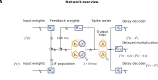
\includegraphics{media/chapters/04_temporal_tuning/spatio_temporal_overview.pdf}%
	\kern-158mm\includegraphics{media/chapters/04_temporal_tuning/spatio_temporal_overview_diagram.pdf}\\[0.5cm]
	\includegraphics{media/chapters/04_temporal_tuning/spatio_temporal_analysis.pdf}%
	{\phantomsubcaption\label{fig:spatio_temporal_a}}%
	{\phantomsubcaption\label{fig:spatio_temporal_b}}%
	{\phantomsubcaption\label{fig:spatio_temporal_c}}%
	{\phantomsubcaption\label{fig:spatio_temporal_d}}%
	\caption[Two-dimensional quantities over time in a rank one spatiotemporal network]{
		Two-dimensional quantities over time in a rank one spatiotemporal network.
		\textbf{(A)}~Overview of the network and results for some exemplary inputs $\mathfrak{x}_1(t)$ and $\mathfrak{x}_2(t)$.
		The input signals are fed into a recurrent network where each neuron is tuned to a random linear combination of the inputs, and a linear combination of the \LDN impulse responses for $q = 5$ and $\theta = \SI{1}{\second}$.
		%After filtering the output spike trains, we can decode linear and nonlinear functions over time and space.
		We can approximately decode delayed versions of the inputs (a linear transformation) and the product of the two input signals for $\theta_1 = \theta_2$.
		\textbf{(B)}~For band-limited noise inputs, delayed versions of the both input signal can be decoded with a small mean delay decoding error $\bar E$. Dashed lines are the delay decoding errors for an equivalent Echo State Network (\ESN; \cite{jaeger2004harnessing}).
		\textbf{(C)}~Decoding error (\NRMSE) when systematically decoding delayed multiplication for delays $\theta_1$, $\theta_2$.
		While the resulting error is quite large, it is substantially smaller than what is achievable with linear approximations of four-quadrant multiplication (i.e., an \NRMSE of $100\%$). Decoding delayed multiplication works best for $\theta_1 = \theta_2$.
		For an \ESN, all errors are above $100\%$.
		\textbf{(D)} Normalised singular values of the recurrent weight matrix.
		The matrix is of rank twelve, with the last four singular values being relatively small.
	}
	\label{fig:spatio_temporal}
\end{figure}

Results are depicted in \Cref{fig:spatio_temporal}.
It is possible to decode delayed versions of the individual input signals with similar errors as in previous experiments.
Decoding delayed multiplication generally results in relatively large errors, with a minimum error of $36\%$.
Most notably, errors are minimal along the diagonal, i.e., $\theta'_1 = \theta'_2$.

\paragraph{Discussion}
Decoding errors for off-diagonal $\theta'_1$, $\theta'_2$ pairs being large is due to $\mat E^\mathrm{t}$ being of rank one.
Each neuron is temporally tuned to a linear combination of the spatial input signal dimensions.
For example, for some $\vec e_i$, $\vec e_i^\mathrm{t}$, the neuron is most active if the time-course of the linear combination $\langle \vec e_i, \mathfrak{x}(t) \rangle$ is similar to the time-course described by the function $\langle \vec e_i^\mathrm{t}, \mathfrak{h}(t) \rangle$.

However, using rank one $\mat E_i^\mathrm{t}$, it is impossible to generate neural tuning such that a neuron is tuned to different input dimensions having different temporal behaviour.
As a result, we cannot decode functions that are nonlinear over several time-points.
This is similar to not being able to decode nonlinear functions from neuron populations with axis-aligned spatial encoders (cf.~\Cref{sec:two_layer_intermediate}).
We reach \NRMSEpl below $100\%$ for $\theta'_1 \neq \theta'_2$ when computing delayed multiplication because the product for the closest uniform delay is a decent approximation.


\subsubsection{Delayed multiplication with full rank $\mat E^\mathrm{t}$}

We repeat the above experiment with full rank spatiotemporal encoding matrices $\mat E^\mathrm{t}$.
That is, instead of sampling spatial and temporal encoding vectors $\vec e_i$, $\vec e^\mathrm{t}_i$, we generate random $\mat E^\mathrm{t}$ with Frobenius norm $\| \mat E^\mathrm{t} \|_\mathrm{F} = 1$.
Specifically, we uniformly sample vectors from the hypersphere $\mathbb{S}^{dq}$, and reshape these vectors into matrix form.

\paragraph{Results}

\begin{figure}
	\centering
	\includegraphics{media/chapters/04_temporal_tuning/spatio_temporal_analysis_matrices.pdf}%
	{\phantomsubcaption\label{fig:spatio_temporal_full_a}}%
	{\phantomsubcaption\label{fig:spatio_temporal_full_b}}%
	{\phantomsubcaption\label{fig:spatio_temporal_full_c}}%
	\caption[Decoding delayed multiplication in a network with full rank spatiotemporal encoders]{
		Decoding delayed multiplication in a network with full rank spatiotemporal encoders $\mat E_i^\mathrm{t}$.
		Same architecture as in \Cref{fig:spatio_temporal_a}.
		\textbf{(A)} Decoding delayed versions of the two input dimensions. Note the slightly smaller mean delay decoding error compared to using a rank one spatiotemporal encoding matrix.
		\textbf{(B)} Delayed multiplication decoding errors are approximately uniform for all combinations of $\theta_1$ and $\theta_2$.
		\textbf{(C)} The recurrent weight matrix now possesses $d q = 10$ non-zero singular values.
	}
	\label{fig:spatio_temporal_full}
\end{figure}

Errors for delay decoding and computing delayed multiplication are given in \Cref{fig:spatio_temporal_full}.
Note that the errors for decoding delayed versions of the individual input signals are slightly smaller than before (\Cref{fig:spatio_temporal_full_a}).
The results for computing delayed computation show a drastic improvement (\Cref{fig:spatio_temporal_full_b}).
Errors are between $30\%$ to $40\%$ for all $\theta'_1$, $\theta'_2$ pairs.

\paragraph{Discussion}
Improvements in the linear delay decoding task are due to slight reduction in our solver loss from \cref{eqn:weight_optimise_currents_temporal}; the more diverse tuning facilitates realising the desired tuning in the recurrent connection.
The reduction in error for the delayed multiplication task is as expected.

Finally, note that the recurrent weight matrices are of low rank (\Cref{fig:spatio_temporal_d,fig:spatio_temporal_full_c}).
This suggests that it is possible to realise the same network in the \NEF without temporal tuning.
Indeed, as we show in \Cref{app:spatiotemporal_nef}, this is possible.
However, we must realise a $qd$-dimensional representation in the population; implementing dynamical systems with spiking neurons in such high dimensional spaces can be challenging.
Our approach offers the advantage of biasing the weight solver towards portions of the activity space relevant for a certain input signals and thus results in smaller errors in the delayed multiplication task.

\subsubsection{Example: Recently travelled distance}

\begin{figure}
	\includegraphics{media/chapters/04_temporal_tuning/path_integration.pdf}
	\caption[Decoding the recently travelled distance distance from a spatiotemporal network]{Decoding the recently travelled distance distance from a spatiotemporal network. Same experimental setup as in \Cref{fig:spatio_temporal}, but decoding the distance travelled over the past second instead.
	\textbf{(A)} Random trajectory generated by integrating the input velocities in $x_1$- and $x_2$-direction.
	Highlighted section (black line and coloured circles) corresponds to the time range displayed in \emph{(B)}.
	\textbf{(B)} Input velocities $\dot x_1(t)$ and $\dot x_2(t)$ and the decoded windowed distance $d_{[t - \theta, t]}$.
	Dotted line is the ground-truth. The \NRMSE $E$ is computed after subtracting the mean (without subtracting the mean $E = 8.1\%$).
	Again, \NRMSEpl are far above $100\%$ when using an \ESN (grey dashed line).
	}
	\label{fig:path_integration}
\end{figure}

As a slightly more practical example of a function that could be decoded from a spatiotemporal network, consider the distance an agent has travelled over the past $\theta$ seconds.
For the sake of simplicity, let $\dot x_1(t)$, $\dot x_2(t)$ denote the velocity of the agent in a global coordinate space.
We define the \emph{recently travelled distance} $d_{[t - \theta, t]}$ as
\begin{align*}
	d_{[t - \theta, t]}(\dot x_1, \dot x_2) = \int_{t - \theta}^t \sqrt{\dot x_1(\tau)^2 + \dot x_2(\tau)^2} \,\,\mathrm{d}\tau \,.
\end{align*}

We test decoding this function using the spike data recorded in the experiment with rank one $\mat E_i^\mathrm{t}$.
Results are depicted in \Cref{fig:path_integration}.
We obtain an \NRMSE of $E \approx 22\%$ over $T = \SI{100}{\second}$.
Crucially, using the full rank $\mat E_i^\mathrm{t}$ we obtain $E \approx 26\%$ (data not shown).

\paragraph{Discussion}
This experiment indicates that it can be beneficial to restrict the encoders to a lower rank.
We apply a linear operator (the integral) to a function that is only nonlinear over the same point in time $\tau$---this is exactly the type of function supported by our rank one spatiotemporal encoding matrices.

Overall, our experiments demonstrate that it is possible to realise populations with spatiotemporal tuning in the \NEF; our \emph{spiking} networks even outperform the popular Echo State Network (\cite{jaeger2004harnessing}) by a wide margin.
A next step would be to use this technique to construct a neurophysiologically motivated model of spatiotemporal tuning in the brain.

\pagebreak

\subsection{Adaptive Filters}
\label{sec:adaptive_filter}

\begin{itemize}
	\item Using the spatiotemporal network we can build an adaptive filter that learns to predict a nonlinear dynamical systems!
	\item Example: Pendulum. Input is the torque $\tau(t)$ and the delayed observed angle $\phi(t - \theta)$. Target is actual angle $\phi(t)$
	\item Use PES learning rule
	\item System learns to output the non-delayed angle! $\Rightarrow$ System learns how the torque over time will affect the angle $\Rightarrow$ We are learning the nonlinear dynamics!
	\item Will provide another example (the cerebellum model) in the next chapter.
\end{itemize}

\subsection{Accounting for Neural Dynamics}
\label{sec:temporal_tuning_neural_dynamics}

\begin{itemize}
	\item Can modify eq. 4.7 to account for neural dynamics. Must find input current that produces the intended output current.
	\item Simple for our $n$-LIF neurons, where we know that the passive dendritic tree acts as a series of low-pass filters. More complex all other cases. See Duggins' work.
	\item Simple example: population of \LIF neurons with low firing rates; neural dynamics play a significant role in the overall network dynamics. Implementing an integrator is not successful.
	\item In eq. 4.7 record the output spike train $a$ and the \enquote{neutral} output spike train $a'$ from a $\Delta\Sigma$ modulator. Use least squares to solve for a causal filter that maps from $a$ onto $a'$. Use that in eq. 4.7.
	\item Note that neural dynamics may also be useful; trivial case: if the neuron has some dynamics, then we can easily realise these dynamics.
\end{itemize}


%\clearpage
%\setcounter{section}{3}
%% !TeX spellcheck = en_GB

\section{Applications to Artificial Neural Networks}
\label{sec:applications_to_ml}

The Legendre Memory Unit (LMU)---originally proposed by \citet{voelker2019lmu}---is a building block for spatiotemporal computing in deep neural networks.
The LMU, just like our models of spatiotemporal biological neuron populations, is a dynamical system that intrinsically performs stream-to-stream processing.
At its core, each LMU consists of a recurrent linear layer implementing the LDN, and a nonlinear layer transforming the LDN state.
By harnessing the ability of the LDN to approximate a sliding window spectrum of length $\theta$, the LMU can, even with little training, integrate information over longer time-spans than competing architectures, while requiring a minimal amount of resources, both in terms of memory and computation.

Crucially, the LMU often outperforms other recurrent neural network architectures in stream processing tasks.
This includes Long Short-Term Memories (LSTMs; \cite{hochreiter1997long}), Gated Recurrent Units (GRUs; \cite{chung2014empirical}) and Echo State Networks (ESNs; \cite{jaeger2004harnessing}).
The LMU performance has been verified for synthetic benchmarks (\cite{voelker2019}, Chapter~6.2; \cite{voelker2019lmu}; \cite{gu2020hippo}), as well as real-world applications such as keyword spotting \citep{blouw2021hardware}, bird song classification \citep{gupta2021comparing}, and natural language processing (NLP; \cite{chilkuri2021parallelizinga}; \cite{chilkuri2021parallelizing}).
A recent study on NLP tasks by \citet{chilkuri2021language} suggests that networks based on a variant of the LMU achieve a ten-times higher data efficiency than Transformers \citep{vaswani2017attention}.
According to Chilkuri et al., this is comparable to the improvement offered by Transformers over LSTMs.

The goal of this section is to explore in how far the success of the LMU depends on projecting the input signal onto the \emph{Legendre} polynomials, and to further characterize the LMU time and space complexity.
Specifically, we test how well our modified Fourier system (cf.~\Cref{sec:lti_autoregression}) fares in place of the LDN system.
Given that we are no longer in a biological setting, we furthermore test sliding-window transformations that rely on perfect memory.

%Our results indicate that \emph{any} reasonable orthogonal sliding window transformation results in a comparable performance.
%Switching to a perfect sliding window transformation can sometimes be more efficient and lead to smaller errors than using the LDN.
% while at the same time yielding slightly smaller errors in our benchmark tasks.


\subsection{The Legendre Memory Unit}
\label{sec:lmu}

\begin{figure}[p]
	\centering
	\includegraphics{media/chapters/04_temporal_tuning/04_04/lmu.pdf}%
	{\phantomsubcaption\label{fig:lmu_a}}%
	{\phantomsubcaption\label{fig:lmu_b}}%
	{\phantomsubcaption\label{fig:lmu_c}}%
	{\phantomsubcaption\label{fig:lmu_d}}%
	\caption[Overview of the Legendre Memory Unit]{Overview of the Legendre Memory Unit. See text for more detail. \textbf{(A)} Variant of the LMU network as proposed by \citet{voelker2019lmu}. The important signal paths are highlighted with bold arrows.
	\textbf{(B, C)} The reduced LRGF and FIR LMU (our acronyms) proposed by \citet{chilkuri2021parallelizing}. \textbf{(D)} In practice, multiple LDN systems are stacked a single layer.}
\end{figure}

The original LMU proposed by \citet{voelker2019lmu} is depicted in \Cref{fig:lmu_a}.
Fundamentally, the idea is to project an input $\vec x_t \in \mathbb{R}^d$ onto a scalar $u_t$ by means of an encoding vector $\vec e_{\vec x}$.%
\footnote{Since artificial neural network operate within discretised time, all input \emph{signals} $\mathfrak{x}$ become input \emph{sequences} ${\vec x}_t$.}
This scalar is then fed into a zero-order hold (ZOH) discretised LDN system with input matrix $\mat{\tilde B}$ and feedback matrix $\mat{\tilde A}$.
Specifically, it holds \citep[e.g.,][Section~9.8]{brogan1991modern}:
\begin{align}
	\vec m_{t + 1} &= \mat{\tilde A} \vec m_t + \mat{\tilde B} u_t \,,
	& \mat{\tilde A} &= \exp\left(\frac{\mat A}{N}\right) \,,
	& \mat{\tilde B} &= {\mat A}^{-1} (\mat{\tilde A} - \mat I) \mat B \,,
	\quad\quad \text{where } N \Delta t = \theta \,.
	\label{eqn:ldn_discretisation}
\end{align}
%Here, $N = \theta \Delta t^{-1}$ is the length of the time-window as a number of samples.

Finally, the $q$-dimensional state $\vec m_t$ is passed through a nonlinear layer, resulting in the output $\vec{h}_t \in \mathbb{R}^m$.
Note that Voelker et al.~include all possible connections between the linear and nonlinear layers in the model.
All weight matrices except for $\mat{\tilde A}$, $\mat{\tilde B}$ are trained via backpropagation \citep[e.g.,][Section~5.3]{bishop2006pattern}.
The LTI matrices $\mat{\tilde A}$, $\mat{\tilde B}$ are kept fixed.

\subsubsection{The LRGF and FIR LMU}
\Citet[Section~3.1.3]{chilkuri2021parallelizinga} observes that the added connections outside the main signal path have little to no positive impact on the performance of the system.
In fact, removing these connections altogether---and thus reducing the number of trainable weights---has a net positive impact on the system performance \citep{chilkuri2021parallelizing}.
This leaves the LDN as the only recurrent component in the network (cf.~\Cref{fig:lmu_b}).
\Citet{tsoi1997discrete} refer to such networks as \enquote{locally recurrent, globally feed-forward} (LRGF).

Since the state-space matrices $\mat{\tilde A}$, $\mat{\tilde B}$ are fixed, we can replace the LDN system by a convolution operation (cf.~\Cref{fig:lmu_c}; \cite{chilkuri2021parallelizing}).
Taking advantage of the fact that the LDN impulse response decays rapidly after $N = \theta \Delta t^{-1}$ samples, we can \emph{approximate} the convolution operation using a \emph{finite} impulse response (FIR) filter of length $N$.

Let $\vec u_t = (u_{t - N + 1}, \ldots, u_t)$ be a slice of the input sequence.
We can construct a matrix of $q$ FIR filters $\mat H \in \mathbb{R}^{q \times N}$, such that $\vec m_t \approx \mat H \vec u_t$ is the state of the LDN system at time $t$.
As pointed out by Chilkuri, the $k$th column of $\mat H$ is simply $(\mat H^T)_k = \mat{\tilde A}^k \mat{\tilde B}$.
This is equivalent to the mean impulse response of the continuous system during the $k$th discrete time-step \citep[cf.][]{stockel2021discrete}:
\begin{align}
	(\mat H^T)_k
		&= \frac{1}N \int_{t_0}^{t_1} \! \exp(\mat A \tau) \mat B \,\mathrm{d}\tau =  \mat{\tilde A}^k \mat{\tilde B} \,, \quad\quad \text{where } t_0 = \frac{k}{N}, \quad t_1 = \frac{k + 1}{N} \,.
	\label{eqn:ldn_h_matrix}
\end{align}

Replacing the LTI system with a set of FIR filters makes the network purely feed-forward.
We thus do not have to rely on backpropagation through time \citep[e.g.,][]{werbos1990backpropagation} for training, and can use the FFT to quickly convolve pre-recorded test and training signals with the $q$ FIR filters.
This can vastly improve training throughput on GPUs \citep{chilkuri2021parallelizing}.
Still, once training has completed, we can always switch back to the recurrent implementation---this \emph{may} (see below) be more efficient when performing realtime stream processing.
%and is one of the advantages that also makes Transformer networks more attractive than LSTMs \citep{vaswani2017attention}.

The idea of using FIR filters (i.e., temporal convolutions) in neural networks is by no means new.
In fact, it harkens back to the early days of multi-layer networks \citep[e.g.,][]{waibel1989phoneme,back1991fir} and has lately been repopularised by \citet{bai2018empirical}.
The novelty of the feed-forward LMU lies in using \emph{fixed} FIR filters approximating an \emph{orthogonal} sliding window spectrum, as well as exploiting the duality between the recurrent and feed-forward networks for efficient inference and training.

\subsubsection{LMU layers and spatiotemporal tuning}
When constructing neural networks, we generally stack multiple LMUs into an \emph{LMU layer} (cf.~\Cref{fig:lmu_d}).
That is, the $d$-dimensional spatial input $\vec x_t$ is projected onto $\ell$ LMUs using encoding vectors $\vec e^1_{\vec h}$, $\ldots$, $\vec e^\ell_{\vec h}$.
This results in a vector $\mat m_t$ of $\ell q$ states feeding into a nonlinear layer of $n$ neurons via a weight matrix $\mat W_{\vec m}$.

Importantly, using encoding vectors $\vec e^i_{\vec h}$ is only efficient if the number of LMUs is smaller than the number of spatial input dimensions, i.e., $\ell < d$.
Otherwise, due to the linearity of convolution, we can simply filter each input dimension separately and implicitly learn the encoding vectors as a part of $\mat W_{\vec m}$.
In this case, each row in $\mat W_{\vec m}$ is a vector of length $d q$.
This vector \emph{exactly} corresponds to a flattened version of our encoding matrix $\mat{E}^\mathrm{t}$ (cf.~eq.~\ref{eqn:temporal_encoding_vector}).
Put differently, an LMU layer is a spatiotemporal NEF population with LDN tuning (cf.~\Cref{sec:spatiotemporal}).

% Background:
% -- A single LMU is an LDN LTI system projecting (using a spatial encoder) a d-dimensional spatial input onto an LDN system. The resulting signal of order q is followed by a nonlinear layer; all other possible connections are then added to the network. All weight matrices except for the fixed LDN LTI system are learned. x
% -- Chilkuri shows that most recurrent connections are not required to achieve the same performance; the most impactful recurrence is that of the LDN system. x
% -- Since this connection is not learned, the LTI system can be replaced by a convolution with a set of FIR filters; we are performing a sliding window-spectrum transformation. Dig up the old literature reference on mixing FIR filters with temporal bases x
% -- ==> Network can be trained using purely feed-forward connections; enables faster training and parallelisation on GPUs. What remains is learning the spatial encoder, and the mapping onto the nonlinear layer x
% -- Typically, many LDN systems are stacked. In our terminology, each linear unit is tuned to a certain spatial stimulus (determined by e_h) and to one of the LDN impulse responses. x
% -- Using the LDN system has in this way has several advantages:
%    -- Compresses a potentially long history into $q$ state dimensions; only $q$ numbers need to be kept in memory instead of the entire signal history
%    -- Updating the LDN system state using an Euler step is possible in O(q).
%    -- Footnote: may also be possible for the modified Fourier basis; there is a sliding window transformation for updating the Fourier trafo and information erasure is of rank one.


%The \enquote{Legendre Memory Unit} (LMU)  network architecture in the field of 
%\Citet{voelker2019lmu} demonstrate that a generalised neural network architecture derived from the LDN, the \enquote{Legendre Memory Unit} (LMU), can outperform other recurrent neural network architectures such as Long Short-Term Memories (LSTMs) in a wide variety of tasks.
%Preliminary work by Chilkuri and Eliasmith (publication in preparation) furthermore suggests that most weights in the LMU can be kept constant without negatively impacting the performance of the network.
%Surprisingly, this includes the recurrent connections in the LMU.
%Constant recurrent weights can be replaced by a set of static feed-forward Finite Impulse Response (FIR) filters arranged in a basis transformation matrix $\mat H$.
%This facilitates parallel training, leading to significant speed-ups.
%
%The basis transformation matrix $\mat H$ can be interpreted as a discrete function basis. This report is concerned with characterizing such function bases, including the related \enquote{Discrete Legendre Orthogonal Polynomials} (DLOPs) introduced by \citet{neuman1974discrete}.
%Our goal is to gain a better understanding of the LDN system and to explore whether it could make sense to instead use other discrete function bases.
%
%An exciting application of the 
%
%... This suggests that the component critical to the function of the Legendre Memory Unit is performing some orthogonal basis transformation. In line with our exploration above, realising this transformation recurrently as an LTI system is merely an implementation detail.


\subsection{Computational Efficiency of Evaluating the LDN LTI System}
\label{sec:ldn_computational_efficiency}

The main advantage of using an order $q$ LTI system to approximate a sliding-window spectrum (as in the LRGF LMU) is memory efficiency in \emph{online} stream-to-stream processing applications.
After all, we only need to remember $q$ state dimensions, compared to the last $N = \theta / \Delta t$ input samples when using FIR filters (as in the FIR LMU).
Correspondingly, we can operate the network in regimes where $N \gg q$ without requiring large amounts of memory.
However, there are some trade-offs to consider with respect to computational efficiency.

\subsubsection{FIR filters can be more computational efficient than state-space LTI systems}
On the surface, it may seem as if evaluating a discrete LTI system of order $q$ in every time-step should be computationally more efficient than evaluating $q$ FIR filters.
After all, computing $\vec m_{t + 1} = \mat{\tilde A} \vec m_t + \mat{\tilde B} u_t$ requires $\mathcal{O}(q^2)$ operations per time-step, while computing $\vec m_t = \mat H \vec u_t$, that is, convolving $\vec u_t$ with a set of FIR filters \emph{online}, requires $\mathcal{O}(qN)$ operations, where $N \geq q$.

However, as pointed out by \citet{gardner1995efficient}, online convolution with $q$ FIR filters can be implemented efficiently in about $34 q \log_2(N)$ operations (amortised), albeit at the cost of $\mathcal{O}(N \log(N))$ memory.
Still, this means that for large $q$, using FIR filters can be \emph{computationally} more efficient than evaluating a generic LTI system.

\subsubsection{Euler LDN update}

Fortunately, the LDN system is not a generic LTI system.
In fact, as pointed out by \citet[Figure~6.6]{voelker2019} in the form of a circuit diagram, it is possible to compute the state update in $\mathcal{O}(q)$ operations if we discretise the LDN using an Euler step instead of the ZOH method from \cref{eqn:ldn_discretisation}.
We get the following update equation and transformation matrix $\mat H'$:%
\begin{align}
	\vec m_{t + 1} = \vec m_{t} + \frac{\mat A \vec m_{t} + \mat B u_t}{N} = \mat {\tilde A}' \vec m_t + \mat {\tilde B}' u_t \,,
	\quad \text{where } N \Delta t = \theta
	\quad \text{and} \quad
	((\mat H')^T)_k = (\mat{\tilde A}')^k \mat{\tilde B}' \,.
	\label{eqn:ldn_system_euler}
\end{align}
\begin{algorithm}[t]
	\begin{minipage}{0.98\textwidth}
	\caption[Euler linear time LDN update]{Euler linear time LDN update. The function below takes the current LDN system state $\vec m = (m_1, \ldots, m_q)$, input $u_t$, system order $q$, window-width $\theta$, as well as the time-step $\Delta t$ and computes the state update $\vec m'$ according to \cref{eqn:ldn_system_euler} in $\mathcal{O}(q)$.
	}
	\label{alg:ldn_euler}
	\end{minipage}
	\sffamily\small
	\SetKwBlock{Begin}{function}{end function}
	\Begin(EulerLDNUpdate${(\vec m, u, q, \theta, \Delta t)}$)
	{
		$\nu \gets \Delta t \theta^{-1} \,, \quad \mu_1 \gets \sum\nolimits_{i = 1}^q m_i \,, \quad m_1' \gets m_1 - \nu (\mu_1 - u)$ \\
		\For{$i = 2~\mathbf{to}~q$}
		{
			$k \gets i - 2~\mathbf{if}~i \geq 3~\mathbf{else}~1$\\
			$\mu_i \gets \mu_k - 2 m_{i - 1}$ \\
			$m_i' \gets m_i - \nu (2i - 1)  (\mu_i - (-1)^i u)$
		}
		\Return $(m_1', \ldots, m_q')$
	}
\end{algorithm}%
An algorithm for computing $\vec m_{t + 1}$ in $\mathcal{O}(q)$ time is outlined in \Cref{alg:ldn_euler}; we exploit the fact that (scaling factors aside) two rows $i$ and $i - 2$ only differ in one column $i - 1$ (cf.~\Cref{fig:ldn_example_b}).%
\footnote{Note that \Cref{alg:ldn_euler} is for the \enquote{original} LDN system, i.e., \emph{not} the rescaled version from \cref{eqn:ldn_system}.}

As any textbook on numerically solving differential equations will warn \citep[e.g.,][Chapter~17.1]{press2007numerical}, Euler integration is rarely a good choice.
It introduces instabilities and, with a $\mathcal{O}(\Delta t)$ residual, is rather imprecise for the expended computational effort.
In contrast, the ZOH scheme is an optimal discretisation of the system impulse response (cf.~eq.~\ref{eqn:ldn_h_matrix}).

We characterise the error introduced by Euler discretisation and its asymptotic stability in \Cref{fig:ldn_euler_vs_zoh}.
However, note that---in our case---deviations from the continuous system are irrelevant as long as $\mat H'$ spans an orthogonal basis.
We characterise the \enquote{quality} of the generated transformation matrix $\mat H'$ by the sum $\Sigma$ of its normalised singular values (cf.~\Cref{fig:ldn_euler_vs_zoh_b,fig:ldn_euler_vs_zoh_orth}); this roughly corresponds to the number of intrinsic orthogonal basis functions.

Independent of the error measure, we observe a quadratic relationship between $N$ and $q$ for maintaining a constant error.
In other words, when using the Euler update, increasing $q$ mandates a quadratically higher sampling rate.
This asymptotically negates the effect of switching to a faster update equation.

\subsubsection{Higher order methods}
Choosing higher-order Runge-Kutta methods instead of Euler can substantially reduce errors \citep[Chapter~17.1]{press2007numerical}.
For a Runge-Kutta method of order $p$, the discrete feedback matrix $\mat{\tilde A}^{\{p\}}$ is a truncated matrix exponential \citep[cf.][]{whitney1969more}:
\begin{align*}
	\mat{\tilde A}^{\{p\}} &= \sum_{k = 0}^p \frac{1}{k!} \left( \frac{\mat A}{N} \right)^k & \text{where} \quad \mat {\tilde A}^{\{1\}} = \mat I + \frac{\mat A}{N} = \mat{\tilde A}' \,, \quad \text{and} \quad \mat{\tilde A}^{\{\infty\}} = \exp\left(\frac{\mat A}{N}\right) = \mat{\tilde A} \,.
\end{align*}
Specifically, $\mat{\tilde A}^{\{2\}}$ corresponds to the midpoint method, and $\mat{\tilde A}^{\{4\}}$ to the canonical Runge-Kutta integrator.
Note that the asymptotic complexity of computing $\mat{\tilde A}^{\{p\}} \vec m_t$ is still in $\mathcal{O}(q)$.
Runge-Kutta methods consist of $p$ nested Euler steps, all of which can be evaluated using \Cref{alg:ldn_euler}.

\begin{figure}
	\centering
	\includegraphics{media/chapters/04_temporal_tuning/04_04/ldn_euler_vs_zoh.pdf}%
	{\phantomsubcaption\label{fig:ldn_euler_vs_zoh_a}}%
	{\phantomsubcaption\label{fig:ldn_euler_vs_zoh_b}}%
	\caption[Exploring the effect of Euler discretisation on the LDN impulse response and stability]{
	Exploring the effect of Euler discretisation on the LDN impulse response and stability for different state-space dimensions $q$ and sample counts $N = \theta \Delta t^{-1}$.
	Circled numbers correspond to the $(N, q)$-pairs in \Cref{fig:ldn_euler_vs_zoh_orth} below. Thin dashed line to the left indicates $N < q$.
	\textbf{(A)} NRMSE between the ZOH and Euler basis transformation matrices $\mat H$, $\mat H'$ (eqs.~\ref{eqn:ldn_discretisation},~\ref{eqn:ldn_system_euler}) and an $\mat H'$ computed using Euler's method.
	\textbf{(B)} Asymptotic stability and basis quality.
	Points above the black line are asymptotically unstable, the Euler system possesses a growth factor $|1 + \lambda_i / N| > 1$.
	Coloured background is the sum of the (normalised) singular values $\Sigma$ of $\mat H'$ divided by the same quantity for $\mat H$ at this point.
	A value of $100\%$ indicates that the spanned basis is as expressive as the one obtained with ZOH discretisation.
	}
	\label{fig:ldn_euler_vs_zoh}
\end{figure}

\begin{figure}
	\centering
	\includegraphics{media/chapters/04_temporal_tuning/04_04/ldn_euler_vs_zoh_orth.pdf}
	\caption[Orthogonality of the ZOH and Euler LDN basis transformation matrix]{
	Orthogonality of the ZOH and Euler LDN basis transformation matrix for $q = 20$.
	Each plot is the result of multiplying \emph{(A)} the ZOH based $\mat H$ or \emph{(B)} Euler based $\mat H'$ with its own transpose.
	Dark red cells corresponds to an entry of $-1$, dark blue cells to $1$.
	$\Sigma$ is the sum of the normalised singular values for each $\mat H$ or $\mat H'$; this roughly indicates the number of \enquote{hidden} orthogonal basis functions (optimally $\Sigma = q$).
	\textbf{(A)}~The ZOH based basis transformation matrix $\mat H$ is nearly orthogonal for all $N$.
	\textbf{(B)}~The Euler based $\mat H'$ requires a twenty times larger $N$ to reach the same degree of orthogonality.
	}
	\label{fig:ldn_euler_vs_zoh_orth}
\end{figure}

\begin{figure}
	\centering
	\includegraphics{media/chapters/04_temporal_tuning/04_04/ldn_higher_order_vs_zoh.pdf}%
	\caption[Exploring the effect of higher order discretisation on the LDN basis quality]{
	Exploring the effect of higher order discretisation on the LDN basis quality and stability.
	Same plot as \Cref{fig:ldn_euler_vs_zoh_b}, but for \textbf{(A)} the midpoint integrator (a second-order Runge-Kutta method) or \textbf{(B)} the fourth-order Runge-Kutta integrator. Both perform substantially better than Euler's method.
	}
	\label{fig:ldn_higher_order_vs_zoh}
\end{figure}

We analyse higher order methods in \Cref{fig:ldn_higher_order_vs_zoh}.
Switching to the midpoint integrator makes a much wider range of $(N, q)$-pairs usable compared to Euler.
Further increasing the order to $p = 4$ has no appreciable effect.%
\footnote{Technically, Euler's method reaches slightly higher relative $\Sigma$ above $100\%$ (up to $103\%$). 
We believe that this is mostly due to the poor discretisation adding noise to $\mat H'$.
The practical benefit of this is likely negligible.}
Crucially, using a higher-order integrator does not affect contour line curvature. $N$ must still be in $\mathcal{O}(q^2)$ to maintain a constant basis quality.

\subsubsection{Efficient modified Fourier system update}

An efficient Euler state update algorithm exists for the modified Fourier LTI system as well.
In the continuous case, the feedback matrix is the difference between $\mat A_\mathrm{F}$, a matrix describing a set of harmonic oscillators, and an information erasure dampening term $\mat \Gamma_\mathrm{F}$ (cf.~eq.~\ref{eqn:information_erasure_approx}).
The dampening term $\mat \Gamma_\mathrm{F}$ is an outer product $\vec e(\theta) \otimes \vec d(\theta)$, and hence $\mat \Gamma_\mathrm{F} \vec m$ can be computed in $\mathcal{O}(q)$.
Moreover, $\mat A_\mathrm{F}$ merely consists of a series of $2 \times 2$ block matrices along the diagonal; correspondingly, computing $\mat A_\mathrm{F} \vec m$ is also in $\mathcal{O}(q)$.

The error characteristics for using the Euler update differ slightly from those of the LDN (cf.~\Cref{fig:mod_fourier_higher_order_vs_zoh,fig:modified_euler_stress}).
The system is highly unstable when using Euler (not depicted); however, when using a higher-order Runge-Kutta update, the system generates an expressive basis for a wide range of $q$ and $N$.
Still, $N$ remains slightly superlinear in $q$ (i.e., $N \approx q^{\frac{4}3}$).

\begin{figure}
	\includegraphics{media/chapters/04_temporal_tuning/04_04/mod_fourier_higher_order_vs_zoh.pdf}
	\caption[Effect of higher order discretisation on the modified Fourier basis]{Effect of higher order discretisation on the modified Fourier basis. Same analysis as in \Cref{fig:ldn_euler_vs_zoh,fig:ldn_higher_order_vs_zoh}, however, for the modified Fourier system.
	Only odd $q$ are included in the analysis.
	\textbf{(A)} Compared to the LDN, a large portion of the space is unstable when using the midpoint method.
	The contour lines no longer describe a strictly quadratic relationship between $q$ and $N$, and a large portion of the space generates an expressive basis.
	\textbf{(B)} No asymptotic instabilities are visible when using the fourth-order Runge-Kutta solver; $N$ is \emph{almost} linear in $q$.
	Markers correspond to \Cref{fig:modified_euler_stress}.
	}
	\label{fig:mod_fourier_higher_order_vs_zoh}
\end{figure}

\begin{figure}
	\includegraphics{media/chapters/04_temporal_tuning/04_04/modified_euler_stress.pdf}%
	\caption[Integrating the Modified Fourier Basis using Runge-Kutta]{Integrating the Modified Fourier Basis using Runge-Kutta.
	Each line corresponds to the impulse response of one of $q = 101$ state dimensions. The system is stable even for small $N$ to $q$ ratios.
	}
	\label{fig:modified_euler_stress}
\end{figure}


%\subsubsection{Exploiting LDN basis low-pass characteristics}
%
%This quadratic dependency between $N$ and $q$ negates some of the computational efficiency gains from switching to the $\mathcal{O}(q)$ update.
%After all, processing an entire window of length $\theta$ now effectively requires $\mathcal{O}(q^3)$ operations.
%
%\begin{figure}
%	\centering
%	\includegraphics{media/chapters/04_temporal_tuning/04_04/ldn_spectrum.pdf}%
%	{\phantomsubcaption\label{fig:ldn_spectrum_a}}%
%	{\phantomsubcaption\label{fig:ldn_spectrum_b}}%
%	{\phantomsubcaption\label{fig:ldn_spectrum_c}}%
%	\caption[LDN basis power spectrum and low-pass characteristics]{LDN basis power spectrum and low-pass characteristics.
%	\textbf{(A)} Power spectrum for different $q$ assuming $\theta = 1\,\mathrm{s}$. The LDN system acts as a strong low-pass filter.
%	\textbf{(B)} Measuring the NRMSE $E$ when removing frequencies above $\hat f$ in a white noise test signal $u(t)$ before representing it in the LDN basis. Data are the mean over $1001$ test signals with $N = 1000$ samples. \textbf{(C)} Extracing the bandlimit frequencies~$\hat f$ for different $q$ from \emph{(B)} that result in a certain representation error $E$ (coloured lines).
%	}
%	\label{fig:ldn_spectrum}
%\end{figure}
%
%Taking the low-pass characteristic of the LDN basis into account, we find that we can apply a hard bandlimit with cutoff $\hat f$ to the input without changing the representation much (\Cref{fig:ldn_spectrum_a,fig:ldn_spectrum_b}).%
%\footnote{One could argue that the fact the the LDN is not a \emph{perfect} low-pass filter may be beneficial in machine learning applications; after all, some information about the higher frequencies is retained and could be extracted by the network.
%However, our experiments below with the sliding Fourier spectrum---which acts as a perfect low-pass filter---suggest that the high frequencies likely play a lesser role.}
%Crucially, the relationship between $q$ and $\hat f$ is \emph{sublinear} (\Cref{fig:ldn_spectrum_c}).
%It can be more time efficient to low-pass filter the input signal, downsample to the Nyquist frequency, i.e., $N \geq 2 \hat f$, and to use the original $\mathcal{O}(q^2)$ ZOH state update.
%Since $\hat f$, and thus $N$, are sublinear in $q$, we need fewer than $\mathcal{O}(q^3)$ operations to filter a window of length~$\theta$.
%
%One caveat of the downsampling technique is the inevitably introduced latency, making it less suited for realtime applications such as robotics.
%However, as we discuss next, we can take this idea further to derive an---in theory---optimal sliding window transformation that is asymptotically optimal both with respect to memory and computation.


\subsection{Efficient Sliding-Window Spectrum Transformations}
\label{sec:efficient_sliding_window}

The superlinear dependency between $N$ and $q$ for Runge-Kutta state updates implies that we effectively only reach a time complexity between $\mathcal{O}(q^{2.3})$ and $\mathcal{O}(q^3)$ over a window period $\theta$ with $N$ samples.
Moreover, and independent of the discretisation method, remember that we only \emph{approximate} a sliding-window spectrum (\Cref{sec:sliding_window_lti}) if we use an order $q$ LTI system.
This is due to ringing caused by not being able to losslessly reconstruct the history of non-bandlimited inputs from the state $\vec m_t$ when performing information erasure (eq.~\ref{eqn:information_erasure_discrete}; \Cref{fig:construct_lti_erasure}).

For discrete sliding-window transformations, these artefacts can be avoided at the cost of recording the input history $\vec u_t$.
In this case, we no longer need to rely on $\vec m_t$ to approximate a delayed version of the input, and can use a discrete version of \Cref{lem:rectangle_window} to realise a perfect window.
Of course, this requires $\mathcal{O}(N)$ memory and may be infeasible for some applications.

Crucially, for some discrete bases, keeping $\vec u_t$ in memory allows us to construct a \emph{perfect} sliding-window transformation with $\mathcal{O}(qN)$ operations per window period $\theta$, where $N$ is fully independent of $q$.
Below, we discuss the discrete Haar wavelets and the sliding discrete Fourier transformation.
We compare these bases to other sliding transformations in the next section.
%This is better than using the \citet{gardner1995efficient} general-purpose \emph{online} FIR convolution, which requires $\mathcal{O}(q N \log(N))$ time and $\mathcal{O}(N\log(N))$ memory.

\subsubsection{Haar Wavelets}

\begin{figure}
	\centering
	\includegraphics{media/chapters/04_temporal_tuning/04_04/haar_basis.pdf}%
	\kern-156.73mm\includegraphics{media/chapters/04_temporal_tuning/04_04/haar_basis_overlay.pdf}%
	\caption[Visualisation of the orthonormal discrete Haar wavelets]{Visualisation of the orthonormal discrete Haar wavelets.
	\emph{Left:} Discrete basis transformation matrix $\mat W$ for $q = N = 32$. Blue is positive, red negative.
	\emph{Right:} Visualisation of the first eight rows in $\mat W$.
	Arrows correspond to the transitions mentioned in the text.
	}
	\label{fig:haar_basis}
\end{figure}

One particular set of discrete basis functions (\Cref{def:discrete_function_basis}) famous for allowing efficient state updates are the \emph{Haar wavelets} depicted in \Cref{fig:haar_basis} \citep{haar1910zur}.
Curiously, a discrete Haar transformation $\mat W \vec u$ with $\mat W \in \mathbb{R}^{q \times N}$ can be computed in $\mathcal{O}(N)$ \citep{kaiser1998fast}, and the sliding spectrum can be updated in $\mathcal{O}(q)$ per sample.

To see this, assume that we store both our current state $\vec m_t$ and the last $N$ input samples $\vec u_t = (u_{t - N + 1}, \ldots, u_{t})$ in memory.
Sliding one of the discrete basis functions $W_i$ over $\vec u_t$, there are at most three samples in the input history that cross a transition point (arrows in the figure) and thus influence the value of $\vec m_t$.
Instead of re-convolving with $W_i$ and $\vec u_t$ in every time-step, we update $\vec m_t$ by accounting for the transitioning samples.

\subsubsection{Sliding Discrete Fourier Transformation (SDFT)}

Similar $\mathcal{O}(q)$ update algorithms can be obtained for the discrete Fourier and cosine basis (cf.~\Cref{sec:function_bases}), namely the sliding discrete Fourier (SDFT; \cite{springer1991sliding,jacobsen2003sliding}) and cosine transformation (SDCT; \cite{kober2004fast}).
Particularly, the SDFT is given as (using real instead of complex coefficients):
\begin{align}
	&\begin{aligned}
		m^{2k - 1}_t &= m^{2k -1}_{t - 1} \cos(f_k) - m^{2k}_{t - 1} \sin(f_k) - u_{t - N} + u_{t}\,, \\
		m^{2k}_t &= m^{2k - 1}_{t - 1}    \sin(f_k) \, + m^{2k}_{t - 1} \cos(f_k) \,,
	\end{aligned} & \quad\quad \text{where} \quad f_k &= \frac{2 \pi k}{N} \,,
	\label{eqn:sdft}
\end{align}
where $m_t^{2k - 1}$ and $m_t^{2k}$ are the real and imaginary coefficients belonging to the frequency term $f_k$.
Note the similarity to a harmonic oscillator LTI system with an additional delayed input, akin to our perfect continuous LTI rectangle window in \Cref{lem:rectangle_window}.%
\footnote{Note that, in contrast to the Haar basis, computing the SDFT does not require random access to the signal history $\vec u_t$. This drastically reduces the required memory bandwidth.}

\newcommand{\symLTI}{\includegraphics{media/chapters/04_temporal_tuning/04_04/sym_lti.pdf}}
\newcommand{\symSDT}{\includegraphics{media/chapters/04_temporal_tuning/04_04/sym_sdt.pdf}}
\newcommand{\symFIR}{\includegraphics{media/chapters/04_temporal_tuning/04_04/sym_fir.pdf}}

\begin{table}[p]
	\caption[Time and space complexity of different sliding transformations]{Time and space complexity of different sliding transformations.
	Memory requirements only take state retained state between updates into account; we exclude constant matrices and filters.
	The column \enquote{window $N$} describes the relationship between $N$ and $q$ (typically $N \geq q$).
	Batch processing corresponds to computing the sliding window spectrum for every point in time for an entire recorded signal $\vec u$ of length $N$ in one go.
	Any sliding-window transformation has an FIR representation and can always fall back to one of the algorithms in the first three rows.
	}
	\label{tbl:time_comparison}
	\small\sffamily
	{
	\centering
	\setlength{\tabcolsep}{8.75pt}
	\begin{tabular}{r l c c c c}
		\toprule
		& & \multicolumn{2}{c}{\textbf{Online} (per sample)} & \multicolumn{1}{c}{\textbf{Batch}} & \textbf{Window} $N$ \\
		\cmidrule(r){3-4}\cmidrule(r){5-5}\cmidrule{6-6}
		\emph{Basis} & \emph{Algorithm} & \emph{Time} & \emph{Memory} & \emph{Time} & \\
		\midrule
		\symLTI, \symSDT, \symFIR~Any & Na\"ive & $\mathcal{O}(qN)$ & $\mathcal{O}(N)$ & $\mathcal{O}(qN^2)$ & $\mathcal{O}(q)$ \\
		\cmidrule{2-6}
		    & FFT\textsuperscript{[1]} & / & / & $\mathcal{O}(qN \log(N))$ & $\mathcal{O}(q)$  \\
		\cmidrule{2-6}
		    & Gardner\textsuperscript{[2]} & $\mathcal{O}(q \log(N))$ & $\mathcal{O}(N \log(N))$ & / & $\mathcal{O}(q)$ \\
		\midrule
		\symLTI~LDN &
			ZOH\textsuperscript{[3]} & $\mathcal{O}(q^2)$ & $\mathcal{O}(q)$ & $\mathcal{O}(q^2 N)$ & $\mathcal{O}(q)$ \\
		\cmidrule{2-6}
		& Euler\textsuperscript{[4]} & $\mathcal{O}(q)$ & $\mathcal{O}(q)$ & $\mathcal{O}(qN)$ & $\approx \mathcal{O}(q^2)$ \\
		\midrule
		\symLTI~Mod. Fourier &
			ZOH\textsuperscript{[3]} & $\mathcal{O}(q^2)$ & $\mathcal{O}(q)$ & $\mathcal{O}(q^2N)$ & $\mathcal{O}(q)$ \\
		\cmidrule{2-6}
		& Euler\textsuperscript{[4]} & $\mathcal{O}(q)$ & $\mathcal{O}(q)$ & $\mathcal{O}(qN)$ & $\approx \mathcal{O}(q^{\frac{4}3})$ \\
		\midrule
		\symSDT~Fourier & SDFT\textsuperscript{[5]} & $\mathcal{O}(q)$ & $\mathcal{O}(N)$ & $\mathcal{O}(qN)$ & $\mathcal{O}(q)$ \\
		\midrule
		\symSDT~Cosine & SDCT\textsuperscript{[6]} & $\mathcal{O}(q)$ & $\mathcal{O}(N)$ & $\mathcal{O}(qN)$ & $\mathcal{O}(q)$ \\
		\midrule
		\symSDT~Haar & FHT\textsuperscript{[7]} & $\mathcal{O}(q)$ & $\mathcal{O}(N)$ & $\mathcal{O}(qN)$ & $\mathcal{O}(q)$ \\
		\bottomrule
	\end{tabular}\\[1em]
	}
	{\footnotesize
		\symLTI~Sliding transformation with a continuous LTI state-space system of order $q$;
		\symSDT~Discrete sliding transformation with a fast update equation;
		\symFIR~Sliding transformation with a FIR filter representation.
		[1] \cite{cooley1965algorithm};
		[2] \cite{gardner1995efficient};
		[3] See \cref{eqn:ldn_discretisation};
		[4] See \Cref{sec:ldn_computational_efficiency};
		[5] \cite{springer1991sliding}; \cite{jacobsen2003sliding};
		[6] \cite{kober2004fast};
		[7] \cite{kaiser1998fast}.
	}
\end{table}

\begin{figure}[p]
	\centering
	\includegraphics{media/chapters/04_temporal_tuning/04_04/sliding_trafo_sigmas.pdf}
	\caption[Comparing the orthogonality of different methods for generating sliding-window spectra]{
		Comparing the orthogonality of different methods for generating sliding-window spectra.
		Plotted is the sum $\Sigma$ of the normalised singular values of the system transformation matrices $\mat H$ for different $q$ (at $N = 1000$).
		When using sliding discrete transformations (\symSDT) or simple a set of arbitrary FIR filters (\symFIR), it holds $\Sigma = q$.
		The quality of the basis generated by the LDN and the modified Fourier system (\symLTI) is suboptimal.
	Note that $\Sigma \approx 0.88q$ for the modified Fourier basis (for odd $q$); the slope of $88\%$ is close to the percentage by which the individual state dimensions were slowed down ($90\%$).
	}
	\label{fig:sliding_trafo_sigmas}
\end{figure}

%Crucially, since the truncated Fourier basis possesses perfect low-pass characteristics with cutoff frequency $\hat f$ at $2 \hat f = q - 1$, we require, by the Nyquist-Shannon sampling theorem \citep{shannon1949communication}, $q$ samples to cover a window period $\theta$.
%Correspondingly, we only need to store $q$ samples in memory for implementing the delay line.%
%\footnote{In practice, some headroom is required, i.e., we should have $N > q$ samples per window period; this way, the downsampler can be simpler. This does not change the asymptotic complexity since $N$ can be linear in $q$.}
%Of course, this requires that the input is downsampled to $q$ samples per $\theta$.
%Luckily, down- and upsampling are well studied aspects of digital signal processing with efficient solutions \citep[Chapter~4]{oppenheim2009discretetime}.
%
%\begin{figure}
%	\centering
%	\includegraphics{media/chapters/04_temporal_tuning/04_04/optimal_sliding_window_trafo.pdf}
%	\caption[A sliding Fourier transformation with optimal memory and time requirements]{A sliding Fourier transformation with optimal memory and time requirements. This system performs a sliding basis transformation while not requiring more than $\mathcal{O}(q)$ space and $\mathcal{O}(qN)$ time per sliding window period $\theta$, where $N$ can be on the order of $q$.
%	\textbf{(A)} The input signal is downsampled to (more than) $q$ samples per $\theta$ and convolved with the windowed Fourier basis. If so desired, the $q$ signals can be upsampled to match the original rate.
%	This may be important if there are subsequent nonlinear transformations, as in the LMU.
%	\textbf{(B)} In the simplest case, a downsampler is a low-pass filter passing on a fraction of the input samples.
%	\textbf{(C)} Convolution with the windowed Fourier basis can be computed efficiently using \cref{eqn:sdft}; these equations describe an LTI system with an input delay.
%	}
%	\label{fig:optimal_sliding_window_trafo}
%\end{figure}
%
%Correspondingly, as is depicted in \Cref{fig:optimal_sliding_window_trafo}, we can envision a system with $\mathcal{O}(q)$ memory complexity and a $\mathcal{O}(qN)$ time complexity for processing a single time-window of length $\theta$ \emph{online}, where $N \geq q$ may be linear in $q$.
%Depending on the quality of the downsampler, the system implements the windowed Fourier transformation with little distortion.
%The main downside of such a system---aside from the more complex implementation and larger constant factors---is that resampling introduces a small delay.


\subsection{Experiments}
\label{sec:lmu_experiments}

So far, we have seen several alternatives to the LDN system used in the Legendre Memory Unit.
As is summarised in \Cref{tbl:time_comparison}, these systems can be implemented in different ways, each with different characteristics in terms of time and space complexity, and different degrees to which they realise an orthogonal function basis (\Cref{fig:sliding_trafo_sigmas}).

To explore how well these systems actually perform in a neural network context, we repeat two experiments from the original LMU paper \citep{voelker2019lmu}; specifically, the psMNIST and Mackey-Glass tasks.
Our goal is to explore in how far changing the sliding-window transformation affects the performance of the LMU in comparison to the LDN variant.
Readers interested in studies comparing the LMU to other neural network architectures are kindly referred to the beginning of this section, where we provide several references.

Our results indicate that the basis choice has a significant, but small effect on the system performance.
The power of the LMU architecture stems from using a \emph{fixed} and \emph{orthogonal} temporal projection; the particular shape and quality of this projection are secondary.
Practitioners should select a transformation from \Cref{tbl:time_comparison} that suits their particular constraints.

\subsubsection{psMNIST}

\begin{figure}
	\includegraphics{media/chapters/04_temporal_tuning/04_04/psmnist_overview_overlay.pdf}%
	\kern-158mm\includegraphics{media/chapters/04_temporal_tuning/04_04/psmnist_overview.pdf}%
	\caption[Overview of the psMNIST task and our network architecture]{Overview of the psMNIST task and our network architecture.
	Input images are randomly permuted and serialised into a stream of pixels presented over time.
	After all $N = 784$ pixels have been fed into the network, the network must output the correct one-hot coded classification.
	In our particular case $q = 468$ and $n = 346$ for a total of \num{166000} weights.}
	\label{fig:psmnist_overview}
\end{figure}

The MNIST dataset \citep{lecun1998gradientbased} contains $28 \times 28$ pixel greyscale images of hand-written digits between zero and nine.
The task is to classify the digits; state-of-the-art classification accuracies are above $99\%$ \citep{baldominos2019survey}.

The permuted sequential MNIST (psMNIST) task has originally been proposed by \citet{le2015simple}.
The idea is to turn the MNIST dataset into a benchmark for the memory capacity of recurrent neural networks.
Specifically, each image is treated as a sequence $\vec u$ of $N = 784$ pixels.
Each pixel is fed one-by-one into the network in consecutive timesteps.
Once the final sample has been processed, the system must correctly classify the digit.
To eliminate spatial correlations in the input, a random but fixed permutation $\pi$ is applied to the samples (cf.~\Cref{fig:psmnist_overview}).
The input signal is thus of the form $\vec u = (u_{\pi(1)}, \ldots, u_{\pi(784)})$.

\paragraph{Additional constraints}
The psMNIST task as described above is a little under-defined.
Specifically, two additional constraints should be met.
First, the network should use less state memory than is required to just store the whole image \citep{voelker2019lmu}, and, second, support \emph{serial execution} \citep{chandar2019nonsaturating}.
In other words, the network must produce correct classifications over time, even if multiple input signals are concatenated.

Implementing temporal convolution as FIR filters of length $N$ (cf.~\Cref{sec:lmu}) intrinsically fulfils the serial execution constraint, but violates the memory constraint.
Each filter requires access to the past $N$ samples; we essentially just compute the inner product between each of the $q$ FIR filters and the input.
The point of using the LDN or modified Fourier system impulse response is that same convolution can be performed by an LTI system of order (and thus memory) $q < N$ within the recurrent LRGF LMU network.%
\footnote{Note that both the LDN and modified Fourier system impulse response produce ringing artefacts that extend beyond the first $N$ samples (cf.~\Cref{fig:modified_euler_stress}), that is, there is some interaction between two consecutively presented input images.
We ignore this to be consistent with the way the psMNIST task is typically evaluated in the literature.
However, we take ringing into account in the Mackey-Glass experiment.}
However, the results for our $\mathcal{O}(N)$ memory transformations should be taken with a grain of salt.

\paragraph{Methods}
Our network architecture is similar to the setup used by \citet{voelker2019lmu}.
We provide an overview of the model in \Cref{fig:psmnist_overview}; the code describing the network can be found in \Cref{app:lmu_code}.
We apply a set of $q = 468$ FIR filters to the $N = 784$ input samples.
The filter output is passed through a 50\% dropout layer for regularisation \citep{hinton2012improving}, followed by $n = 346$ ReLU neurons that non-linearly processes the temporal representation.
The neural activities are linearly projected onto a one-hot coded output.
Note that $q = 468$ is motivated by the amount of memory used by \citet{chandar2019nonsaturating}.

As is customary, we split the MNIST dataset into $50\,000$ training and $10\,000$ validation samples.
We use a categorical cross-entropy loss function and an Adam optimizer \citep{kingma2015adam} with default parameters over $100$ epochs at a batch size of $100$.
The reported test errors are computed for the epoch with the smallest validation error.
For $q = 468$ the number of trainable parameters is $\approx\num{166000}$.
Per default, the FIR filters are fixed and initialised with one of the previously discussed discretised basis transformations with window length $N = 786$ (i.e., the number of pixels).
The LTI systems are discretised using zero-order hold.

As a point of comparison, we repeat the experiments with randomly initialised FIR filters, as well as enabled learning for the FIR filter matrices.
Learning the FIR filters adds another \num{350000} parameters and is supposed to test in how far our original transformations are optimal.

\begin{figure}
\centering
\includegraphics{media/chapters/04_temporal_tuning/04_04/psmnist_results.pdf}
\caption[Classification accuracies for the psMNIST dataset using different sliding-window transformations]{Classification accuracies for the psMNIST dataset using different sliding-window transformations.
Depicted are standard box-plots over $101$ trials for each basis, each with a different random permutation $\pi$ and weight initialisations. Box corresponds to the first and third quartile; whiskers are the minimum/maximum after outlier rejection; outliers are depicted as circles.
Dashed black line is the mean, notches correspond to the bootstrapped $95\%$ confidence interval.
Numerical values and significance levels are provided in \Cref{tbl:psmnist_results}.
Symbols correspond to possible algorithms from \Cref{tbl:time_comparison}.
}
\label{fig:psmnist_results}
\end{figure}

\begin{table}
	\caption[Test accuracies for the psMNIST experiment]{Test accuracies for the psMNIST experiment for $q = 468$. Data over $n = 101$ trials and $100$ epochs. Q1 and Q3 are the 25- and 75-percentile, respectively. The best three results are highlighted in each column (darker colours are better).}
	\label{tbl:psmnist_results}
	\centering\small\sffamily
	\setlength{\tabcolsep}{7.25pt}
	\begin{tabular}{r  r r r r  r r r r}
	\toprule
	& \multicolumn{4}{c}{{\color{skyblue1}$\blacksquare$} \textbf{Fixed convolution}}
	& \multicolumn{4}{c}{{\color{aluminium2}$\blacksquare$} \textbf{Learned convolution}} \\
	\cmidrule(r){2-5}\cmidrule(l){6-9}
	\emph{Basis} &
	\emph{Mean} &
	\emph{Median} &
	\emph{Q1} &
	\emph{Q3} &
	\emph{Mean} &
	\emph{Median} &
	\emph{Q1} &
	\emph{Q3} \\
	\midrule
		\symLTI~LDN &
			98.49\% &
			98.48\% &
			98.44\% &
			98.55\% &
			 \cellcolor{CornflowerBlue!25}{98.23\%} &
			98.22\% &
			 \cellcolor{CornflowerBlue!25}{98.16\%} &
			 \cellcolor{CornflowerBlue!25}{98.30\%} \\
			\symLTI~Mod.~Fourier &
			98.53\% &
			 \cellcolor{CornflowerBlue!50}{98.54\%} &
			 \cellcolor{CornflowerBlue!25}{98.48\%} &
			98.58\% &
			 \cellcolor{CornflowerBlue!75}{98.24\%} &
			 \cellcolor{CornflowerBlue!50}{98.24\%} &
			 \cellcolor{CornflowerBlue!75}{98.18\%} &
			 \cellcolor{CornflowerBlue!50}{98.31\%} \\
			\symSDT~Fourier &
			 \cellcolor{CornflowerBlue!75}{98.56\%} &
			 \cellcolor{CornflowerBlue!75}{98.56\%} &
			 \cellcolor{CornflowerBlue!75}{98.51\%} &
			 \cellcolor{CornflowerBlue!75}{98.62\%} &
			98.21\% &
			98.21\% &
			98.13\% &
			 \cellcolor{CornflowerBlue!25}{98.30\%} \\
			\symSDT~Cosine &
			 \cellcolor{CornflowerBlue!50}{98.54\%} &
			 \cellcolor{CornflowerBlue!50}{98.54\%} &
			 \cellcolor{CornflowerBlue!50}{98.49\%} &
			 \cellcolor{CornflowerBlue!50}{98.60\%} &
			98.22\% &
			98.22\% &
			 \cellcolor{CornflowerBlue!25}{98.16\%} &
			98.29\% \\
			\symSDT~Haar &
			98.47\% &
			98.46\% &
			98.40\% &
			98.53\% &
			98.22\% &
			98.22\% &
			98.14\% &
			98.29\% \\
			\symFIR~DLOP &
			 \cellcolor{CornflowerBlue!50}{98.54\%} &
			 \cellcolor{CornflowerBlue!50}{98.54\%} &
			 \cellcolor{CornflowerBlue!25}{98.48\%} &
			 \cellcolor{CornflowerBlue!50}{98.60\%} &
			 \cellcolor{CornflowerBlue!25}{98.23\%} &
			 \cellcolor{CornflowerBlue!25}{98.23\%} &
			98.14\% &
			 \cellcolor{CornflowerBlue!25}{98.30\%} \\
			\symFIR~Random &
			98.11\% &
			98.13\% &
			98.05\% &
			98.19\% &
			 \cellcolor{CornflowerBlue!75}{98.24\%} &
			 \cellcolor{CornflowerBlue!75}{98.25\%} &
			 \cellcolor{CornflowerBlue!50}{98.17\%} &
			 \cellcolor{CornflowerBlue!75}{98.32\%} \\
	\bottomrule
	\end{tabular}
\end{table}

\begin{table}
	\newcommand{\sigA}{\ensuremath{\cdot}}
	\newcommand{\sigB}{\ensuremath{\bullet\bullet}}
	\newcommand{\sigC}{\ensuremath{\bullet\!\bullet\!\bullet}}
	\caption[Statistical significance of the psMNiST test accuracies]{Statistical significance of the psMNIST test accuracies. The given significance levels are based on a two-sided Kolmogorov-Smirnov test; $\sigA \correspondsTo p < 0.05$, $\sigB \correspondsTo p < 0.01$, $\sigC \correspondsTo p < 0.001$.}
	\label{tbl:psmnist_significance}
	\centering\small\sffamily
	\setlength{\tabcolsep}{6.2pt}
	\begin{tabular}{r r  c c c c c c c  c c c c c c c}
	\toprule
	& & \multicolumn{7}{c}{{\color{skyblue1}$\blacksquare$} \textbf{Fixed convolution}}
	& \multicolumn{7}{c}{{\color{aluminium2}$\blacksquare$} \textbf{Learned convolution}} \\
	\cmidrule(r){3-9}\cmidrule(l){10-16}
	\emph{Basis} & & (1) & (2) & (3) & (4) & (5) & (6) & (7)  & (1) & (2) & (3) & (4) & (5) & (6) & (7) \\
	\midrule
	\symLTI~LDN & (1) &
		 &
		\sigC &
		\sigC &
		\sigC &
		 &
		\sigB &
		\sigC &
		 &
		 &
		 &
		 &
		 &
		 &
		 \\
		\symLTI~Mod.~Fourier & (2) &
		\sigC &
		 &
		 &
		 &
		\sigC &
		 &
		\sigC &
		 &
		 &
		 &
		 &
		 &
		 &
		 \\
		\symSDT~Fourier & (3) &
		\sigC &
		 &
		 &
		 &
		\sigC &
		 &
		\sigC &
		 &
		 &
		 &
		 &
		 &
		 &
		 \\
		\symSDT~Cosine & (4) &
		\sigC &
		 &
		 &
		 &
		\sigC &
		 &
		\sigC &
		 &
		 &
		 &
		 &
		 &
		 &
		 \\
		\symSDT~Haar & (5) &
		 &
		\sigC &
		\sigC &
		\sigC &
		 &
		\sigC &
		\sigC &
		 &
		 &
		 &
		 &
		 &
		 &
		 \\
		\symFIR~DLOP & (6) &
		\sigB &
		 &
		 &
		 &
		\sigC &
		 &
		\sigC &
		 &
		 &
		 &
		 &
		 &
		 &
		 \\
		\symFIR~Random & (7) &
		\sigC &
		\sigC &
		\sigC &
		\sigC &
		\sigC &
		\sigC &
		 &
		 &
		 &
		 &
		 &
		 &
		 &
		 \\
	\bottomrule
	\end{tabular}
\end{table}

\paragraph{Results}
Results are depicted in \Cref{fig:psmnist_results} and \Cref{tbl:psmnist_results,tbl:psmnist_significance}; learning curves are provided in \Cref{fig:lmu_trajs}.
The modified Fourier, Fourier, cosine and discrete Legendre (DLOP; \Cref{sec:function_bases}) basis outperform the LDN and Haar wavelets slightly but significantly.
The LDN result is state-of-the art for the psMNIST task at about $98.5\%$ accuracy \citep{chilkuri2021parallelizing}.
There is no significant difference between initialisations when learning the convolution; enabling learning on the FIR filters always results in the same, substantially worse performance.

\paragraph{Discussion}
Learned convolutions performing worse is likely a result of the increased parameter count and overfitting to the training data (cf.~\Cref{fig:lmu_trajs}).
Visualising the learned FIR filters (data not shown), we find that they do not differ substantially from their original initialisation.
This suggests that our orthogonal transformations are locally optimal.

Thinking about the FIR filter matrix $\mat H$ purely in terms of a projection $\mat H \vec u$, it is unclear why our systematic bases work better than a random initialisation---after all, this results in an (almost) orthogonal projection as well.
There is a history of successfully applying orthogonal basis transformations such as the discrete Cosine or Haar transform to the MNIST dataset for spatial decorrelation \citep{baldominos2019survey}.
However, these experiments are without pixel permutation; with permutation, spatial decorrelation is an unlikely explanation.

One hint at the worse performance of the random initialisation is our \enquote{orthogonality measure} $\Sigma$ (that is, the sum of the normalised singular values).
For the random FIR filters $\Sigma$ is only about $0.5q$, while we reach higher $\Sigma$ for our other bases (cf.~\Cref{fig:sliding_trafo_sigmas}).


\subsubsection{Mackey-Glass}

\begin{figure}
	\includegraphics{media/chapters/04_temporal_tuning/04_04/mackey_glass_system.pdf}
	\caption[Visualisation of the Mackey-Glass system]{Visualisation of the Mackey-Glass system as used in our benchmark task.
	Left plot shows a short segment of the state evolution, the right plot a 2D delay embedding (delay of $50$ samples).
	\textbf{(A)}~For $\tau \geq 17$ the system behaves mildly chaotically. \textbf{(B)}~For $\tau = 30$ the system is fully chaotic.}
	\label{fig:mackey_glass_system}
\end{figure}

The Mackey-Glass dynamical system \citep{mackey1977oscillation} is a popular benchmark for time-series prediction \citep[cf.][Section 4.3.1]{mendel2017uncertain}.
The goal is to predict the time-course of the following differential equation (cf.~\Cref{fig:mackey_glass_system}).
\begin{align*}
	\dot{\vec u}(t) &= \frac{a u(t - \tau)}{1 + u(t - \tau)^{10}} - b u(t) \quad\quad \text{for} \quad t \geq 0\,,
\end{align*}
where $a = 0.2$, $b = 1.2$.
For $t < 0$ we assume that the state variable $u(t)$ is a Gaussian process with mean $\mu = 1.2$ and standard-deviation $\sigma = 1$.
Notably, the system behaves chaotically if $\tau \geq 17$; that is, small perturbations to the initial state can lead to dramatically different state trajectories.
This makes predicting the system particularly hard.
For our experiment, we construct a network that attempts to predict the time-course of the discretised Mackey-Glass system with $\tau = 30$ for the next fifteen state samples $u_{t + 1}, \ldots, u_{t + 15}$ given the recent state history.

\paragraph{Dataset}
For our experiments, we choose $\tau = 30$.
As a training dataset we generate $400$ Mackey-Glass state trajectories consisting of \num{10000} samples at $\Delta t = 1$ using a fourth order Runge-Kutta integrator; the trajectories are normalised to mean zero and standard deviation one.
All trajectories are different due to the stochasticity of the initial $u(t)$ for $t < 0$.

We randomly extract 100 input sequences of length $117$ followed by a target sequence of length 15 from each trajectory; this results in 40\,000 training samples. We similarly generate \num{10000} validation and \num{10000} test samples.
Training, validation, and test samples are all taken from separately generated trajectories.
The sample length $117$ corresponds to the absolute width of the combined FIR filters in our network; as is illustrated in \Cref{fig:mackey_glass_overview_overlay_b}, only the last $37$ samples are effectively taken into account for the prediction.

\begin{figure}
	\includegraphics{media/chapters/04_temporal_tuning/04_04/mackey_glass_overview.pdf}%
	\kern-158mm\includegraphics{media/chapters/04_temporal_tuning/04_04/mackey_glass_overview_overlay.pdf}\\[0.25cm]
	{\phantomsubcaption\label{fig:mackey_glass_overview_overlay_a}}%
	{\phantomsubcaption\label{fig:mackey_glass_overview_overlay_b}}%
	\caption[Overview of the Mackey-Glass prediction network and dataset]{
		Overview of the Mackey-Glass prediction network and dataset.
		\textbf{(A)} Samples $u_t$ fed into the network pass a series of four LMU layers (here depicted as FIR LMUs); the output is a prediction $\vec{\hat y}_t$ of the next fifteen samples $u_{t + 1}, \ldots, u_{t + 15}$.
		Every sample fed into the network immediately updates the prediction in the output.
		When using the LDN or the modified Fourier system as a sliding transformation, the FIR LMUs can of course be replaced with a corresponding recurrent LRGF LMU.
		\textbf{(B)} Exemplary input-target pair for $\tau = 17$.
		The absolute window of the FIR filters in our network amounts to $117$ samples; samples older than this cannot \emph{possibly} affect the output. However, only the last $37$ samples \emph{effectively} influence the system.
		The longer absolute window ensures that we account for ringing artefacts in the LDN and modified Fourier system (cf.~\Cref{fig:lmu_mackey_glass_filters}).
	}
\end{figure}

\paragraph{Methods}
Our neural network architecture is inspired by \citet{voelker2019lmu} and depicted in \Cref{fig:mackey_glass}.
The relevant code may be found in \Cref{app:lmu_code}.

There are four cascading LMU layers; the last three layers consist of ten stacked sliding-window transformations each.
In contrast to the previous experiment, each transformation uses small $q$ with $N = q$.%
\footnote{Note that a sliding transformation with $q = N$ is lossless, and a potential use-case for an efficient sliding-window spectrum (\Cref{sec:efficient_sliding_window}).
This only requires $2q$ memory and less computation than the LDN or modified Fourier system---we cannot use an efficient Euler update for $q = N$ (\Cref{sec:ldn_computational_efficiency}).}
Specifically, the first LMU layer uses $q_1 = N_1 = 17$, the second and third $q_{23} = N_{23} = 9$, and the final layer $q_{4} = N_4 = 5$.
Assuming that our sliding-transformation implements a perfect rectangle window, this results in the aforementioned \emph{effective} combined window width of $37$.%
\footnote{Specifically, $37 = N_1 + N_2 + N_3 + N_4 - 3$. Each layer \enquote{consumes} $N_i - 1$ samples, and one additional sample is required to obtain a single output sample. See also our discussion in \Cref{app:lmu_code}.}
The absolute window width stems from the impulse response of the LDN and modified Fourier system technically extending beyond $N_i$.
For good measure, we therefore extend the FIR filters to be three times as long as the actual window width.

As in the previous experiment, we compare fixed convolutions, including random initialisations, to a version of the network where the convolutions are initialized in the same way, but then trained during training.
Note that we do not train the extended filters.
The total number parameters is $2750$; another $476$ parameters are added if the convolutions are trained.

We train the network for $100$ epochs with a batch size of $100$ using a standard Adam optimizer.
The final test error is computed for the parameters in the epoch with the smallest validation error.
Our training loss is the MSE, we report the NRMSE.
Note that our results are not directly comparable those in the literature due to using a different $\tau$ and normalisation of the Mackey-Glass dataset.
Our goal is merely to compare different LMU variants.

\paragraph{Results}

\begin{figure}[p]
\centering
\includegraphics{media/chapters/04_temporal_tuning/04_04/mackey_glass_results.pdf}
\caption[Prediction errors for the Mackey-Glass dataset using different sliding-window transformations]{Prediction errors for the Mackey-Glass dataset using different sliding-window transformations. See \Cref{fig:psmnist_results} for a description of the plot.
Numerical values are given in \Cref{tbl:mackey_glass_results}.}
\label{fig:mackey_glass}
\end{figure}

\begin{table}[p]
	\caption[Prediction errors for the Mackey-Glass dataset]{Prediction errors for the Mackey-Glass dataset. Data over $101$ trials after $100$ epochs of training. See \Cref{tbl:psmnist_results} for a description of the table.}
	\label{tbl:mackey_glass_results}
	\centering\small\sffamily
	\setlength{\tabcolsep}{8.75pt}
	\begin{tabular}{r  r r r r  r r r r}
	\toprule
	& \multicolumn{4}{c}{{\color{skyblue1}$\blacksquare$} \textbf{Fixed convolution}}
	& \multicolumn{4}{c}{{\color{aluminium2}$\blacksquare$} \textbf{Learned convolution}} \\
	\cmidrule(r){2-5}\cmidrule(l){6-9}
	\emph{Basis} &
	\emph{Mean} &
	\emph{Median} &
	\emph{Q1} &
	\emph{Q3} &
	\emph{Mean} &
	\emph{Median} &
	\emph{Q1} &
	\emph{Q3} \\
	\midrule
	\symLTI~LDN &
	 \cellcolor{CornflowerBlue!75}{4.32\%} &
	 \cellcolor{CornflowerBlue!75}{4.05\%} &
	 \cellcolor{CornflowerBlue!75}{3.55\%} &
	 \cellcolor{CornflowerBlue!75}{4.98\%} &
	 \cellcolor{CornflowerBlue!25}{4.69\%} &
	 \cellcolor{CornflowerBlue!75}{4.41\%} &
	 \cellcolor{CornflowerBlue!25}{3.84\%} &
	5.45\% \\
	\symLTI~Mod.~Fourier &
	5.27\% &
	5.05\% &
	4.52\% &
	5.77\% &
	4.83\% &
	4.70\% &
	 \cellcolor{CornflowerBlue!50}{3.82\%} &
	5.50\% \\
	\symSDT~Fourier &
	4.99\% &
	4.68\% &
	4.13\% &
	5.49\% &
	4.78\% &
	4.61\% &
	4.05\% &
	 \cellcolor{CornflowerBlue!25}{5.44\%} \\
	\symSDT~Cosine &
	 \cellcolor{CornflowerBlue!25}{4.64\%} &
	 \cellcolor{CornflowerBlue!50}{4.34\%} &
	 \cellcolor{CornflowerBlue!50}{3.75\%} &
	 \cellcolor{CornflowerBlue!50}{5.21\%} &
	 \cellcolor{CornflowerBlue!75}{4.68\%} &
	 \cellcolor{CornflowerBlue!25}{4.48\%} &
	3.91\% &
	 \cellcolor{CornflowerBlue!50}{5.28\%} \\
	\symSDT~Haar &
	4.77\% &
	4.59\% &
	4.03\% &
	5.53\% &
	4.78\% &
	4.63\% &
	 \cellcolor{CornflowerBlue!25}{3.84\%} &
	5.45\% \\
	\symFIR~DLOP &
	 \cellcolor{CornflowerBlue!50}{4.58\%} &
	 \cellcolor{CornflowerBlue!25}{4.43\%} &
	 \cellcolor{CornflowerBlue!25}{3.88\%} &
	 \cellcolor{CornflowerBlue!25}{5.22\%} &
	 \cellcolor{CornflowerBlue!75}{4.68\%} &
	 \cellcolor{CornflowerBlue!50}{4.42\%} &
	 \cellcolor{CornflowerBlue!75}{3.78\%} &
	 \cellcolor{CornflowerBlue!75}{5.23\%} \\
	\symFIR~Random &
	6.46\% &
	6.15\% &
	5.08\% &
	7.34\% &
	5.12\% &
	4.89\% &
	4.19\% &
	5.62\% \\
	\bottomrule
	\end{tabular}
\end{table}

\begin{table}[p]
	\newcommand{\sigA}{\ensuremath{\cdot}}
	\newcommand{\sigB}{\ensuremath{\bullet\bullet}}
	\newcommand{\sigC}{\ensuremath{\bullet\!\bullet\!\bullet}}
	\caption[Statistical significance of the Mackey-Glass test errors]{Statistical significance of the Mackey-Glass test errors. The given significance levels are based on a two-sided Kolmogorov-Smirnov test; $\sigA \correspondsTo p < 0.05$, $\sigB \correspondsTo p < 0.01$, $\sigC \correspondsTo p < 0.001$.}
	\label{tbl:mackey_glass_significance}
	\centering\small\sffamily
	\setlength{\tabcolsep}{6.2pt}
	\begin{tabular}{r r  c c c c c c c  c c c c c c c}
	\toprule
	& & \multicolumn{7}{c}{{\color{skyblue1}$\blacksquare$} \textbf{Fixed convolution}}
	& \multicolumn{7}{c}{{\color{aluminium2}$\blacksquare$} \textbf{Learned convolution}} \\
	\cmidrule(r){3-9}\cmidrule(l){10-16}
	\emph{Basis} & & (1) & (2) & (3) & (4) & (5) & (6) & (7)  & (1) & (2) & (3) & (4) & (5) & (6) & (7) \\
	\midrule

	\symLTI~LDN & (1) &
	 &
	\sigC &
	\sigC &
	 &
	\sigB &
	 &
	\sigC &
	 &
	 &
	 &
	 &
	 &
	 &
	 \\
	\symLTI~Mod.~Fourier & (2) &
	\sigC &
	 &
	\sigB &
	\sigC &
	\sigB &
	\sigC &
	\sigC &
	 &
	 &
	 &
	 &
	 &
	 &
	 \\
	\symSDT~Fourier & (3) &
	\sigC &
	\sigB &
	 &
	\sigA &
	 &
	 &
	\sigC &
	 &
	 &
	 &
	 &
	 &
	 &
	 \\
	\symSDT~Cosine & (4) &
	 &
	\sigC &
	\sigA &
	 &
	 &
	 &
	\sigC &
	 &
	 &
	 &
	 &
	 &
	 &
	 \\
	\symSDT~Haar & (5) &
	\sigB &
	\sigB &
	 &
	 &
	 &
	 &
	\sigC &
	 &
	 &
	 &
	 &
	 &
	 &
	 \\
	\symFIR~DLOP & (6) &
	 &
	\sigC &
	 &
	 &
	 &
	 &
	\sigC &
	 &
	 &
	 &
	 &
	 &
	 &
	 \\
	\symFIR~Random & (7) &
	\sigC &
	\sigC &
	\sigC &
	\sigC &
	\sigC &
	\sigC &
	 &
	 &
	 &
	 &
	 &
	 &
	 &
	 \\
	\bottomrule
	\end{tabular}
\end{table}

Results are depicted in \Cref{fig:mackey_glass} and \Cref{tbl:mackey_glass_results,tbl:mackey_glass_significance}.
Overall, all bases perform similarly, with the LDN outperforming the Fourier and modified Fourier bases.
The modified Fourier basis is significantly worse than all other bases.
The random initialization has by far the highest error, and the LDN, cosine, and DLOP filters result in the lowest error.
Learning the convolution consistently closes the performance-gap between the individual bases.

\paragraph{Discussion}
The cause of the unfavourable performance of the modified Fourier basis is unclear.
We can rule out the ringing artefacts (cf.~\Cref{fig:lmu_mackey_glass_filters})---the performance gap remains after forcing a perfect rectangle window (see \Cref{fig:mackey_glass_ne} and \Cref{tbl:mackey_glass_results_ne,tbl:mackey_glass_ne_significance}).

A possible culprit is that the best-performing bases (i.e., the LDN, DLOP, and cosine basis) are aperiodic, and that even the unmodified Fourier basis performs slightly worse than the other bases.
Using a sub-optimal Fourier basis may thus further reduce the performance to the level observed here.
However, a more detailed analysis is required.

Overall, our results clearly indicate that the basis choice is secondary, and that using fixed orthogonal temporal convolutions can greatly reduce the number of trainable parameters without sacrificing performance.
The particular architecture to choose (e.g., FIR or LRGF LMU), or whether to rely on an order $q$ LTI system instead of an efficient sliding-window transformation solely depends on the particular application.
Limiting constraints are the sampling rate (determining whether a fast Euler update is possible), available memory, as well as latency requirements (i.e., whether to use batch, online, or hybrid processing).
%
%\clearpage
%\setcounter{section}{4}
%% !TeX spellcheck = en_GB

\section{Conclusion}
\label{sec:temporal_tuning_conclusion}

We proposed a linear model of spatiotemporal tuning as a generalisation of the \NEF dynamics principle (cf.~\Cref{sec:nef_dynamics}; \cite{eliasmith2003neural}, Chapter~8).
In particular, we incorporated a model of temporal tuning in visual cortex \citep[cf.][]{carandini1999linearity} into the \NEF tuning curve equation.
This way, we can construct biologically plausible spiking neural networks that approximate spatiotemporal functions.
We furthermore pointed out that there is a direct connection between the Legendre Memory Unit (\LMU; \cite{voelker2019lmu}), a promising component for stream-to-stream processing in artificial neural networks, and our spatiotemporal \NEF populations.

Conceptually, our most important argument is that it is possible to systematically harnesses diverse temporal tuning as a resource for temporal computation.
That is, the pronounced dynamical properties of biological neural networks are an important part of the computation that is being performed.
Just as neural nonlinearities and diverse \emph{spatial} tuning can be exploited to compute non-temporal functions, it is possible to exploit the dynamics inherent to biological networks to form temporal bases, from which we can in turn decode functions \emph{through time}.
We focused on synaptic filters as a primary source of dynamics, but neural dynamics and even signal propagation delays could similarly be taken into account.

In line with the \NEF dynamics principle, we suggested that recurrent connections play a crucial role in forming diverse temporal tuning.
While feed-forward connections can recombine existing temporal tuning, they are inherently limited by the fixed filters along the signal path.

Solving for weights that realise desired dynamics through recurrent connections is often accomplished through computationally intensive methods such as backpropagation through time \citep{werbos1990backpropagation} or, in the context of modelling neurobiological systems, FORCE (\cite{sussillo2009generating,nicola2017supervised}; see \cite{voelker2019}, Section~2.2.4 for a review).
With our approach, we instead rely on the \enquote{self-fulfilling prophecy} inherent to the \NEF.
We assume that each pre-population already possesses its desired tuning, and use this fact to realise the post-population tuning.
Curiously, the pre- and post-population are the same for recurrent connections, and solving for weights is a matter of minimising a linear least-squares problem.

Although our new formalisms are in some ways equivalent to the \NEF dynamics principle, they offer a new perspective when modelling neurobiological networks.
Modellers can specify the temporal tuning of a neuron population independently of its spatial tuning down to individual neurons.
We use our least-squares optimisation problem to realise this desired tuning.
An example of this is the use of bell-shaped temporal encoders depicted in \Cref{fig:linearly_independent_tuning}.

This way, our work eliminates a limitation of the \NEF dynamics principle.
While it is possible to directly take empirical neurophysiological data into account when selecting spatial tuning properties (i.e., using the representation principle) and solving for spatial connection weights (i.e., using the transformation principle), the dynamics principle typically---with some exceptions---requires modellers to provide closed-from differential equations.
Providing such closed-form equations is further complicated when attempting to realise dynamics in networks with heterogeneous or higher-order synapses \citep{voelker2018improving}.
Our approach suggests a way to better take empirical data into account and to automate the process of solving for weights, even in networks with complex recurrences (cf.~\Cref{sec:lti_complex_networks,sec:solve_dynamics_nonlinear_neurons}).

Finally, we presented a method for constructing low-order \LTI systems generating temporal bases using an \enquote{information erasure} technique.
This approach can be used to derive the \LTI system underlying the Legendre Delay Network (\LDN; \cite{voelker2018improving}), but can similarly be applied to other bases as well.
We suggested a \enquote{modified Fourier basis}, that outperforms the \LDN system in several benchmark tasks, and when mapped onto our spiking neural networks can be used to realise time-cells in biological network models.

Furthermore, the modified Fourier basis could be particularly attractive for stream processing in artificial neural networks, where, due to an efficient Runge-Kutta state update, we effectively require $\mathcal{O}(q)$ space and $\mathcal{O}(q^{2.3})$ time for processing a window of length $\theta$.
This is a substantial improvement over the \LDN used in the \LMU which we found to require $\mathcal{O}(q^3)$ time.

\subsubsection{Future work}

A central shortcoming of our work is a lack of mathematical stability guarantees.
While we argued that our recurrent networks will realise the desired dynamics \emph{if} they can be realised perfectly, it is unclear what happens in cases where this condition is broken.
We observe in practice that our networks are typically well-behaved (i.e., not asymptotically unstable); however, it would be interesting to augment our weight solver with techniques from system identification that guarantee stability \citep[cf.][]{verhaegen2007filtering}.

Another aspect that we have only considered in the context of our adaptive filter experiment, is using the temporal tuning curve paradigm to realise nonlinear tuning.
This is easily possible using the \NEF dynamics principle \citep[Chapter~8]{eliasmith2003neural} and also not a hard limitation of our temporal tuning curve approach.
In fact, our general definition of a temporal tuning curve is oblivious to the specific type of dynamics (cf.~\Cref{def:temporal_tuning_curve}).
Rather, the problem is one of finding a good mathematical formalisation; linear temporal encoders $\mathfrak{e}_i$ offer an intuitive parametrisation of temporal tuning curves that we would have to give.

Taking intrinsic neural dynamics into account is another aspect of the work presented here that requires further research.
While linearly approximating neural dynamics was successful for the simple neuron models tested here, it would be interesting to extend this to more complex neuron models, potentially incorporating work by \citet{duggins2017incorporating}.
It could similarly be interesting to model transmission delays using temporal tuning, and demonstrate that our methods can capture low-level phenomena such as auditory coincidence detection in the brain stem \citep[Chapter~31]{kandel2012principles}.

In order to disseminate our methods to researchers modelling neurobiological systems, it would be interesting to integrate our approaches into a software tool such as the Nengo spiking neural network simulator \citep{bekolay2014nengo}.
An interesting engineering challenge would be to define a convenient \API for temporal tuning that ties well into the existing system.
In this respect, it would also be beneficial to find ways to more efficiently solve the least-squares problem defined in \cref{eqn:weight_optimise_currents_temporal} by relying on spectral decompositions.
